\documentclass[9pt]{article}
\usepackage[english]{babel}
\usepackage{amsmath,amsthm}
\usepackage{amsfonts}
\usepackage{graphicx}
\usepackage[margin=0.2in]{geometry}
\newcommand{\setlinespacing}[1]{\setlength{\baselineskip}{#1 \defbaselineskip}}
\newcommand{\doublespacing}{\setlength{\baselineskip}{2.0 \defbaselineskip}}
\newcommand{\singlespacing}{\setlength{\baselineskip}{\defbaselineskip}}
\newcommand{\A}{{\cal A}}
\newcommand{\h}{{\cal H}}
\newcommand{\s}{{\cal S}}
\newcommand{\W}{{\cal W}}
\newcommand{\BH}{\mathbf B(\cal H)}
\newcommand{\KH}{\cal  K(\cal H)}
\newcommand{\Real}{\mathbb R}
\newcommand{\Complex}{\mathbb C}
\newcommand{\Field}{\mathbb F}
\newcommand{\RPlus}{[0,\infty)}
\newcommand{\norm}[1]{\left\Vert#1\right\Vert}
\newcommand{\essnorm}[1]{\norm{#1}_{\text{\rm\normalshape ess}}}
\newcommand{\abs}[1]{\left\vert#1\right\vert}
\newcommand{\set}[1]{\left\{#1\right\}}
\newcommand{\seq}[1]{\left<#1\right>}
\newcommand{\eps}{\varepsilon}
\newcommand{\To}{\longrightarrow}
\newcommand{\RE}{\operatorname{Re}}
\newcommand{\IM}{\operatorname{Im}}
\newcommand{\Poly}{{\cal{P}}(E)}
\newcommand{\EssD}{{\cal{D}}}
\newcommand{\field}[1]{\mathbb{#1}}
\newcommand{\C}{\field{C}}
\newcommand{\R}{\field{R}}
\newcommand{\script}[1]{\mathcal{#1}}
\newcommand{\fall}{\; \forall \;}
\newcommand{\exts}{\; \exists \;}
\newcommand{\mbf}[1]{\mathbf{#1}}
\newcommand{\binomial}[2]{\biggl( \begin{array}{c}  #1 \\ #2  \\ \end{array} \biggr) }
\newcommand{\fderiv}[2]{ \frac{d}{ d #1} \: #2}
\newcommand{\sderiv}[2]{ \frac{d^2}{ d^2 #1} \: #2}
\newcommand{\pfderiv}[2]{ \frac{\partial}{ \partial #1} \: #2}
\newcommand{\psderiv}[2]{ \frac{\partial^2}{ \partial^2 #1} \: #2}
\newcommand{\mat}[1]{\mathbf{#1}}
\DeclareSymbolFont{AMSb}{U}{msb}{m}{n}
\DeclareMathSymbol{\dblz}{\mathalpha}{AMSb}{"5A}
\DeclareMathSymbol{\dblr}{\mathalpha}{AMSb}{"52}
\DeclareMathSymbol{\dblt}{\mathalpha}{AMSb}{"54}
\DeclareMathSymbol{\dblq}{\mathalpha}{AMSb}{"51}
\DeclareMathSymbol{\dbln}{\mathalpha}{AMSb}{"4E}
\DeclareMathSymbol{\dblf}{\mathalpha}{AMSb}{"46}
\DeclareMathSymbol{\dblc}{\mathalpha}{AMSb}{"43}
\DeclareMathSymbol{\dbld}{\mathalpha}{AMSb}{"44}
\theoremstyle{plain}
\newtheorem{thm}{Theorem}[section]
\newtheorem{cor}[thm]{Corollary}
\newtheorem{lem}[thm]{Lemma}
\newtheorem{prop}[thm]{Proposition}
\theoremstyle{definition}
\newtheorem{defn}{Definition}[section]
\theoremstyle{remark}
\newtheorem{rem}{Remark}[section]
\numberwithin{equation}{section}
\renewcommand{\theequation}{\thesection.\arabic{equation}}
\begin{document}
\title{Regression of KL Software Distribution   }
\author{KL Software Libraries}
\date{Wed Jun 11 17:15:47 2014
}
\maketitle
\textbf{ KL Library test output.  This LaTex file and the associated diagrams are produced by the KL software libraries.}
\subsubsection{Matrix Quick Check <double>}
QueryPerformanceCounter  =  0.0942156
\subsubsection{Linear Regression atan data 3x1}
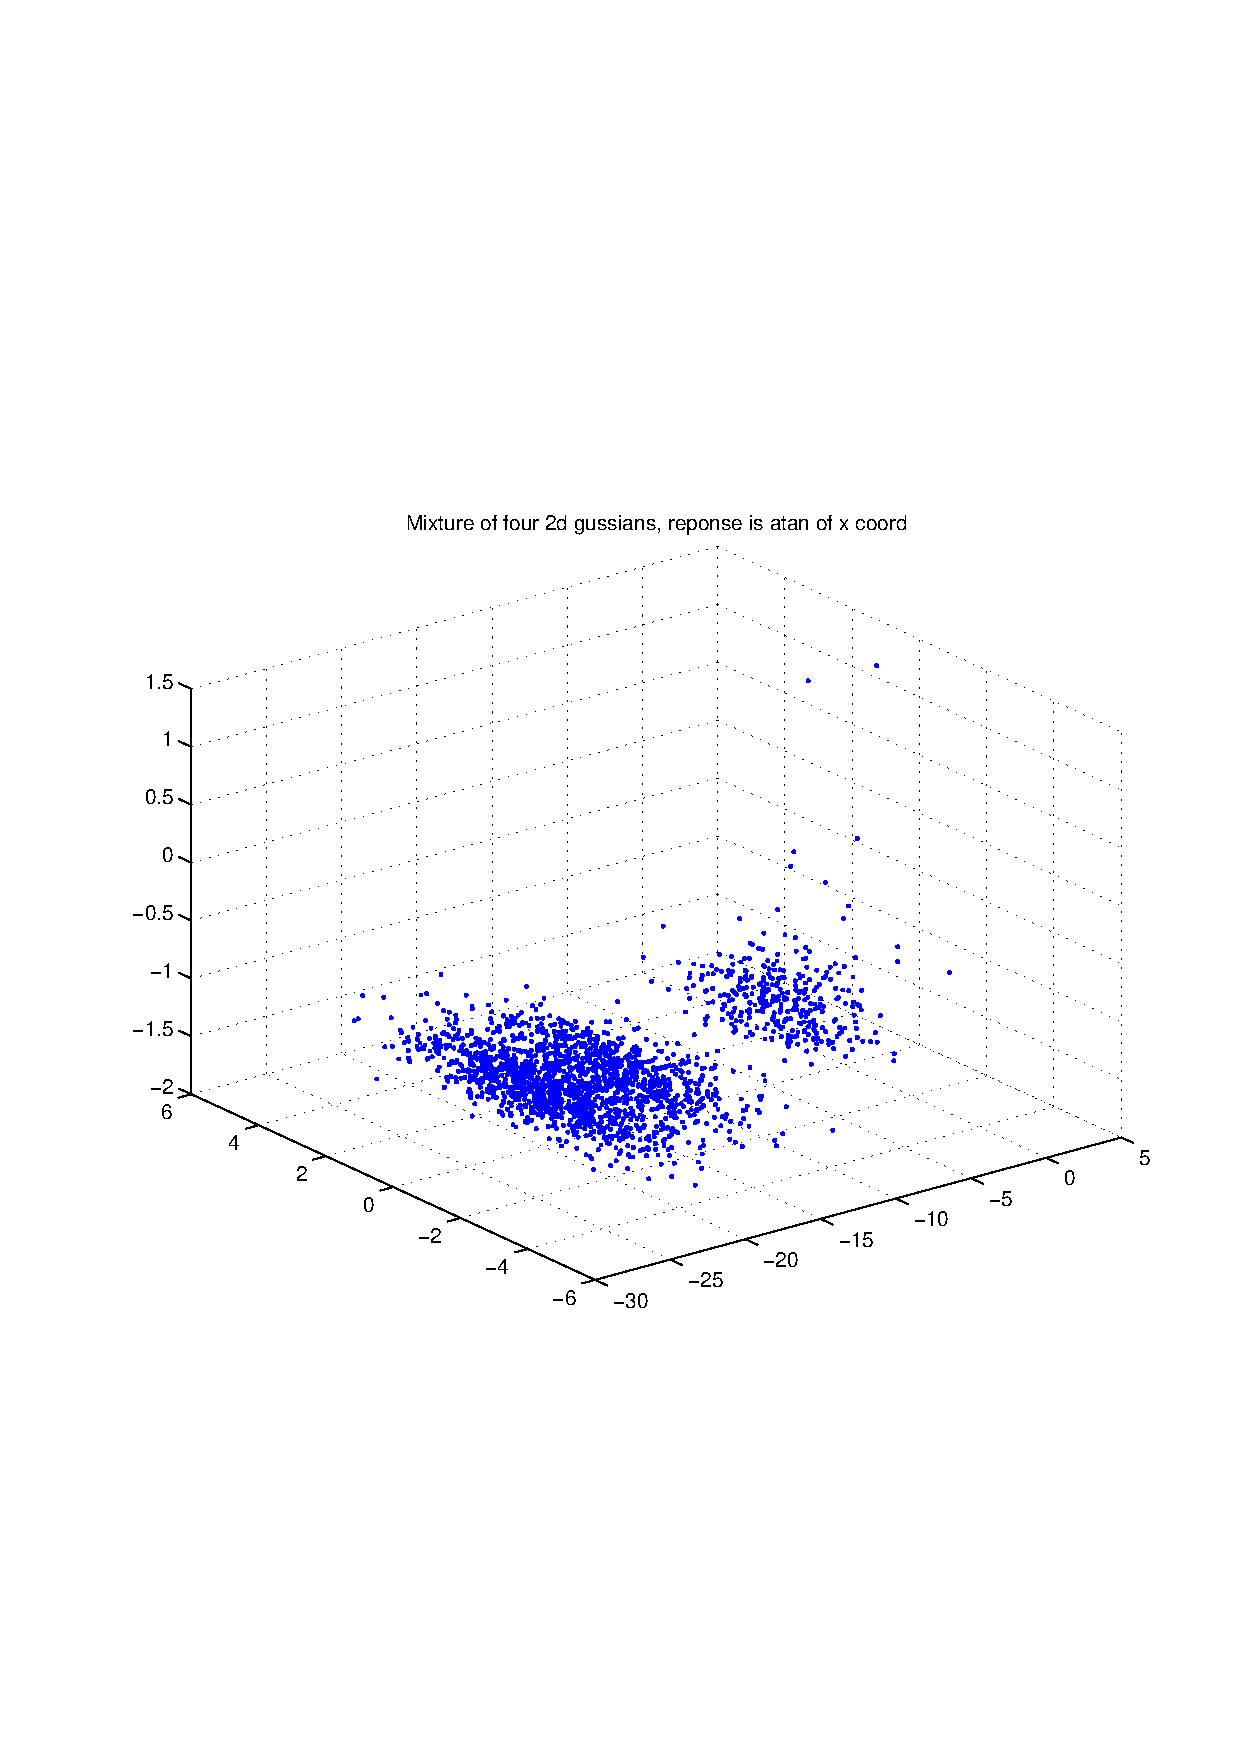
\includegraphics[width=10.0cm,height=10.0cm]{AtanDataSet.pdf}

\subsubsection{3 x 1 Linear Regression}
Sample size = 4000

Number of features = 3

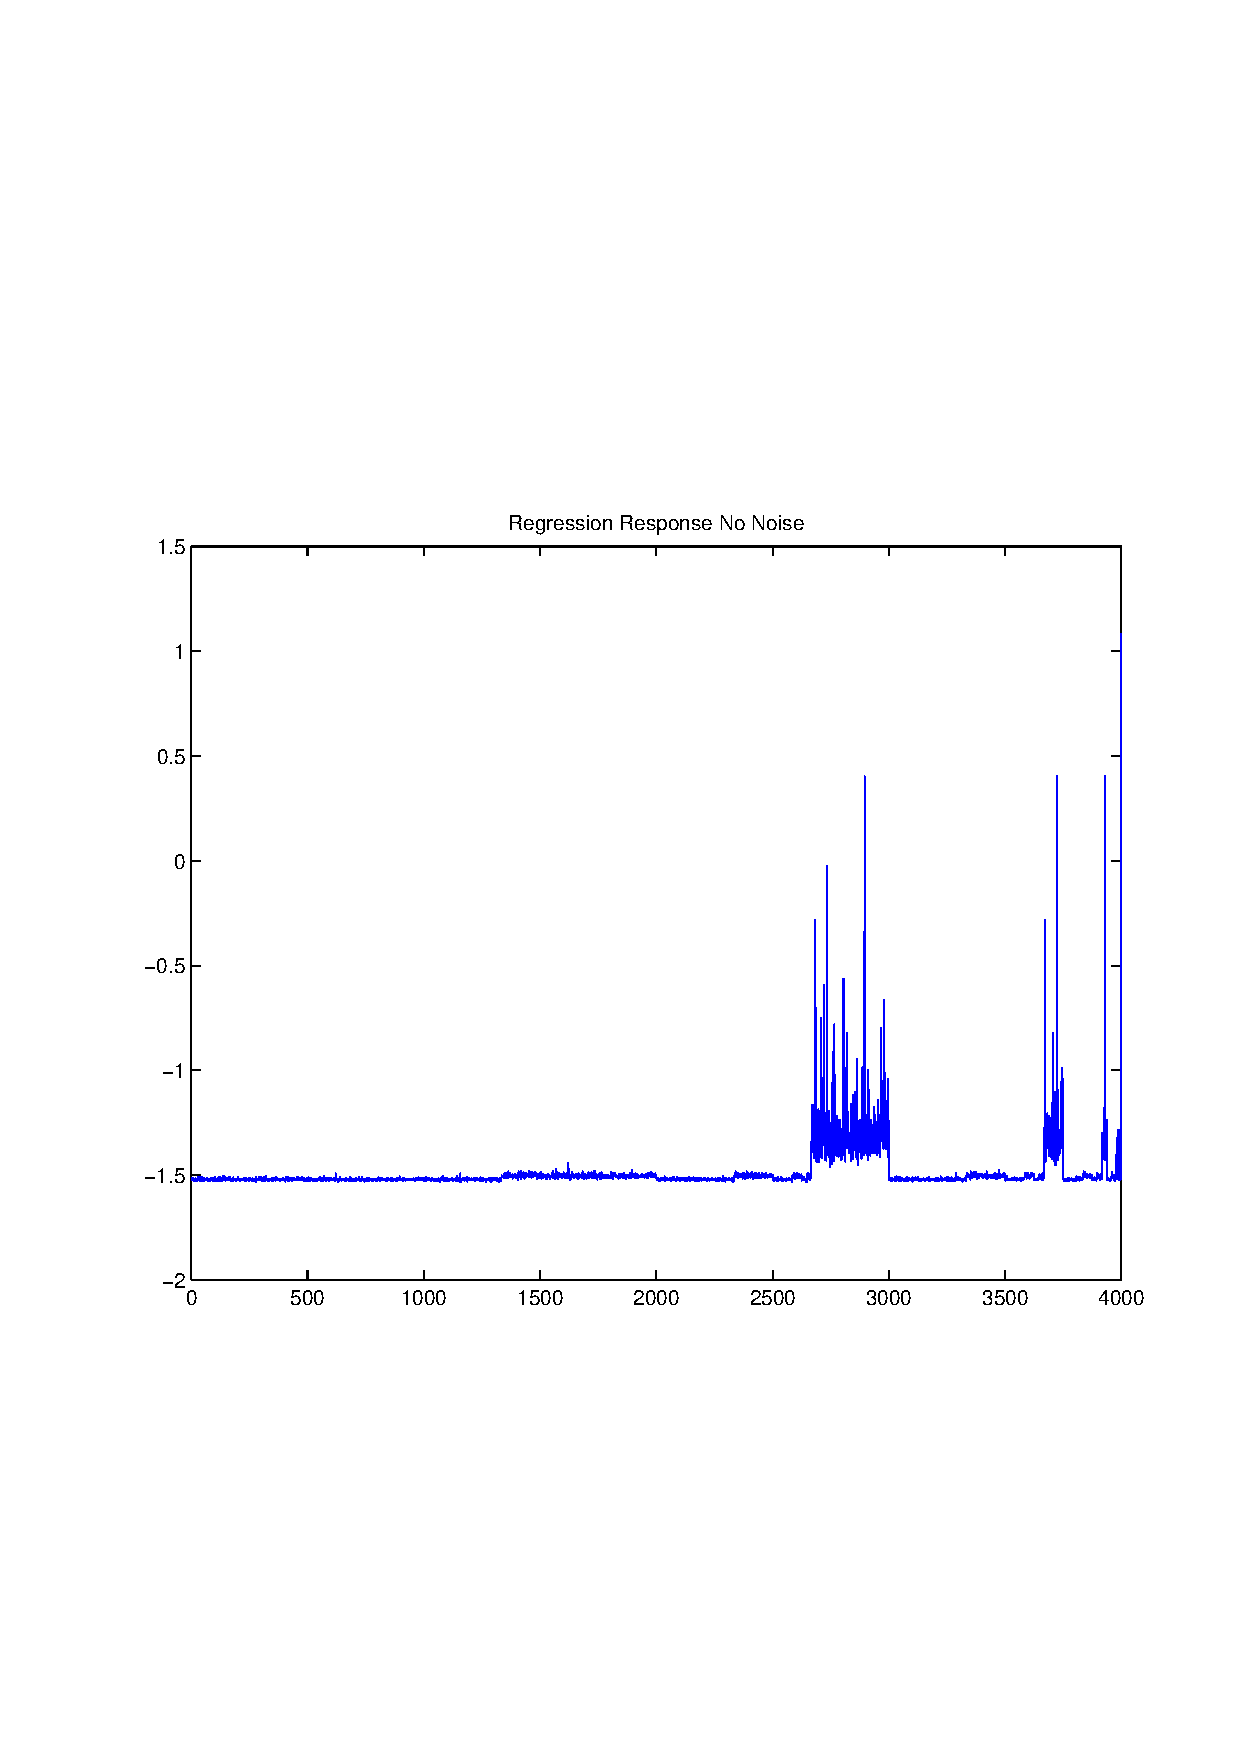
\includegraphics[width=10.0cm,height=10.0cm]{AtanDataSet_regression_response_no_noise.pdf}

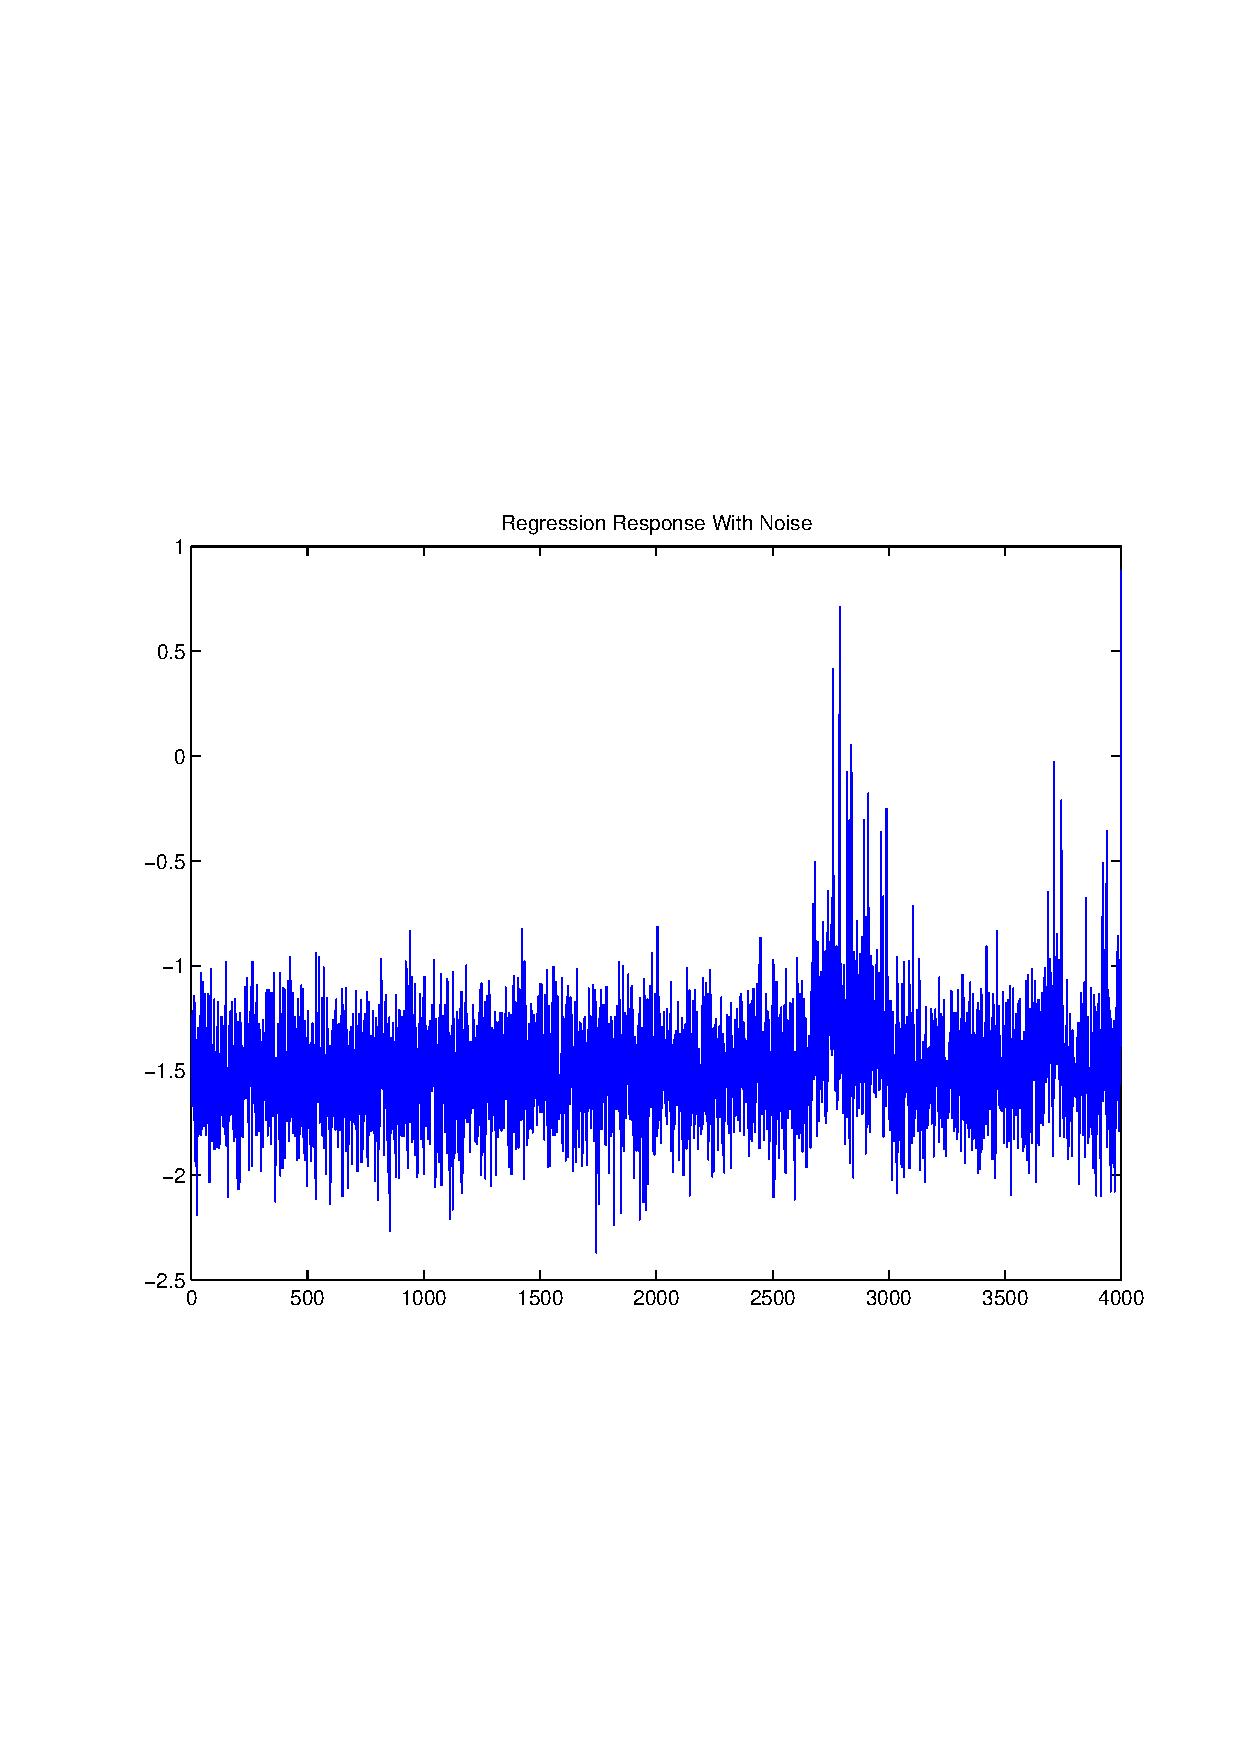
\includegraphics[width=10.0cm,height=10.0cm]{AtanDataSet_regression_response_with_noise.pdf}

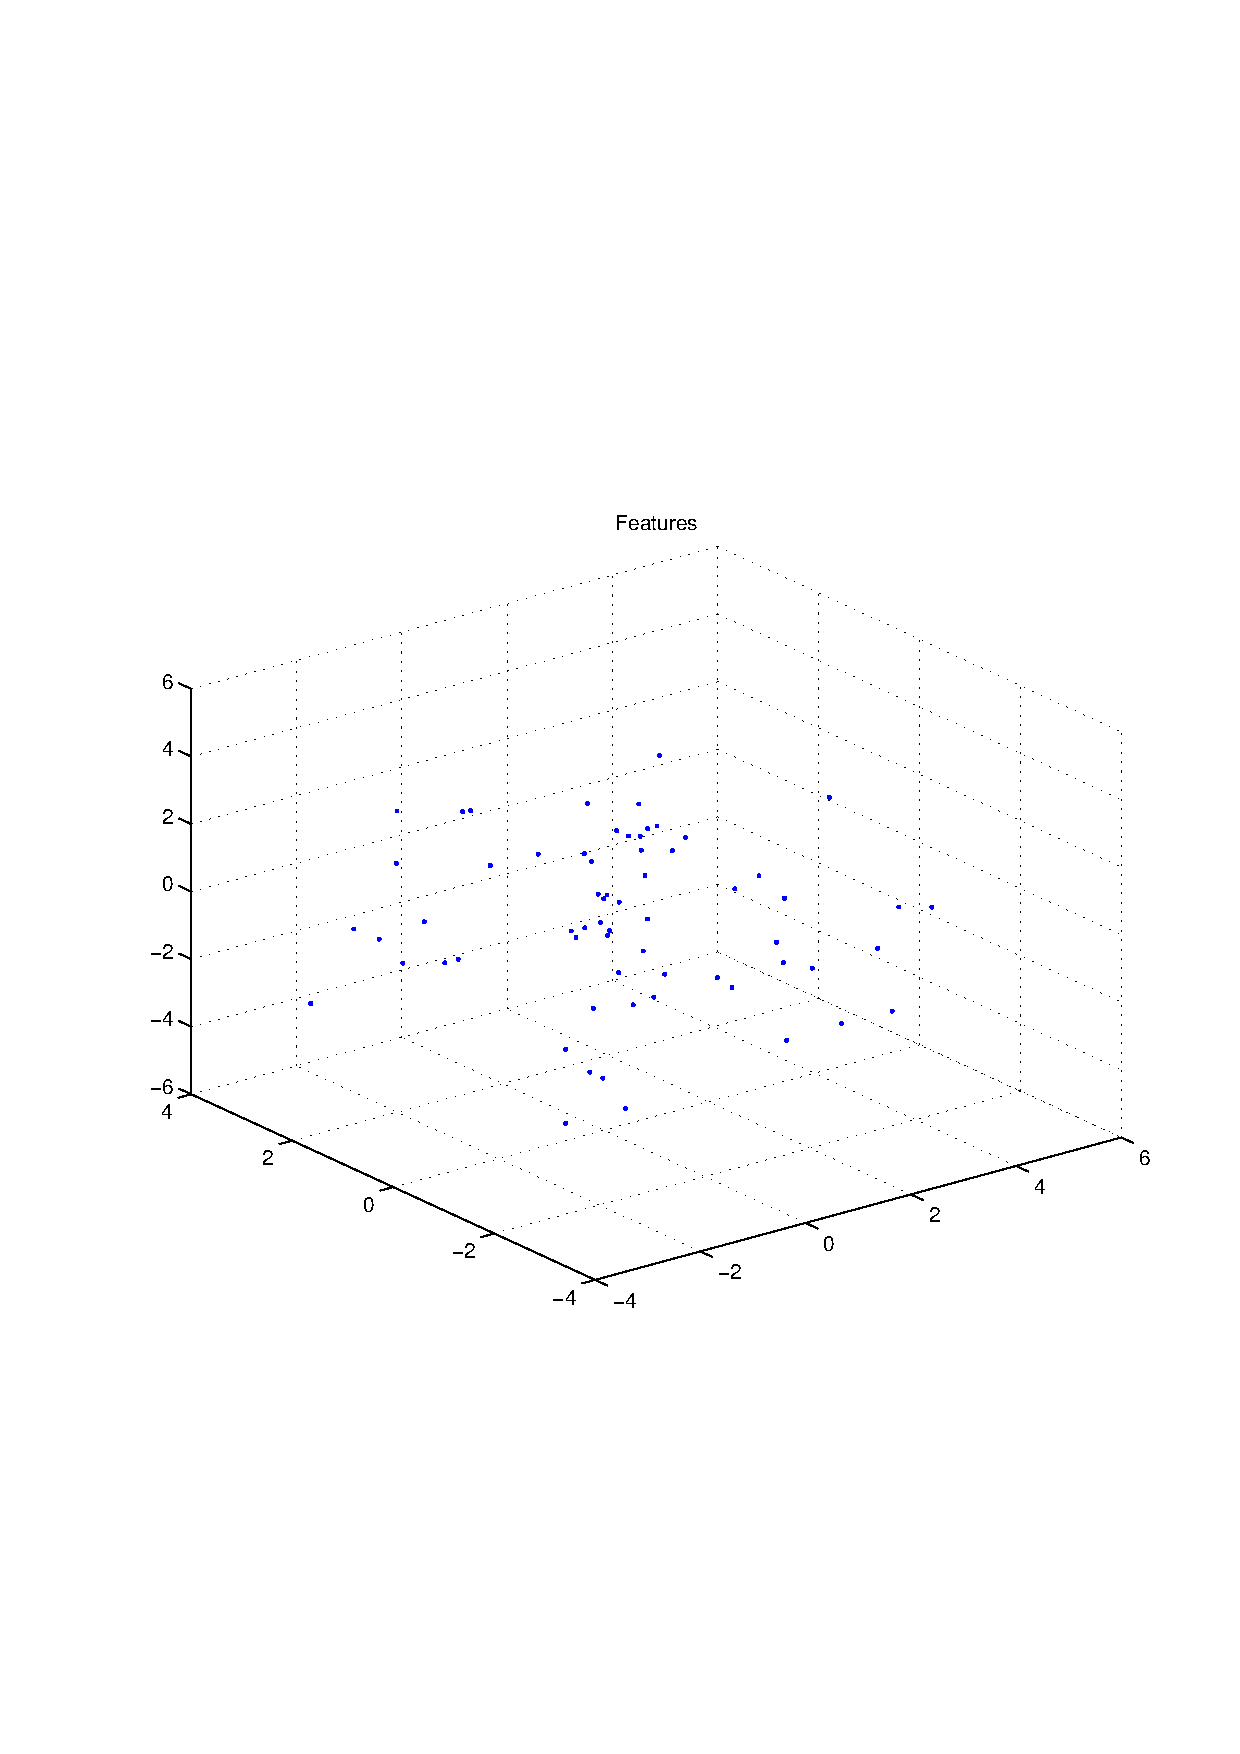
\includegraphics[width=10.0cm,height=10.0cm]{regression_features.pdf}

Response
-1.43558
-1.65343
-1.34873
1.63367
-1.31093
-1.32839
-1.14858
1.59711
-1.31524
-1.13051
-1.47703
1.45914
-1.74079
-1.48531
-1.17919
0.943028
-1.17579
-1.36576
-1.79584
1.20843
-1.42756
-1.52325
-1.15705
0.983525
-1.47594
-2.17027
-1.06462
1.4786
-1.45546
-1.75201
-1.32926
1.52868
-1.80263
-1.76786
-1.36364
1.6598
-1.25446
-1.47169
-0.675556
1.12508
-1.17223
-1.37614
-0.922932
1.39014
-1.23079
-1.7602
-1.33478
1.14606
-1.52018
-1.05918
-1.10612
1.6164
-1.55399
-1.73762
-1.11404
1.23008
-1.45499
-1.12058
-1.46975
1.17491
-1.4912
-1.75872
-1.32721
1.21151
-1.81559
-1.29404
-1.40796
0.710418
-1.53206
-1.47235
-0.842391
1.77246
-1.74334
-1.22019
-1.50826
0.970074
-1.6066
-2.00913
-0.940261
1.26188
-1.44232
-1.51714
-1.509
1.75586
-1.3428
-0.990459
-1.31601
1.40007
-1.85214
-1.54569
-1.33242
1.45191
-1.38176
-1.5054
-1.09398
1.30926
-1.37947
-1.20956
-0.87535
1.01838
-1.82333
-1.50642
-1.26002
1.07026
-1.69961
-1.81389
-1.17413
1.37874
-1.61565
-1.61764
-1.7267
1.34405
-1.17747
-1.35874
-1.55338
1.24631
-1.80878
-1.39462
-1.5153
1.35672
-1.66511
-1.59614
-1.32169
1.19446
-1.80322
-1.53993
-1.49496
1.40463
-1.41512
-1.23116
-1.52401
1.18986
-1.70239
-1.65028
-1.37801
1.30427
-1.5836
-1.76468
-1.61582
1.18129
-1.66025
-1.43344
-0.746884
1.15845
-1.80318
-1.17884
-1.62266
1.67755
-1.62732
-1.75534
-1.59286
1.34885
-1.47231
-1.68816
0.167335
1.31471
-1.68436
-1.48031
-2.00933
0.914838
-1.3933
-1.30036
-1.19218
1.13187
-1.68182
-1.57373
-1.05172
1.66979
-1.71997
-1.49008
-1.24076
1.29397
-1.36715
-1.16016
-0.760762
1.38696
-1.63695
-1.77131
-1.37383
1.3283
-1.49324
-1.57593
-1.65795
1.23477
-1.48273
-1.80733
-0.981937
1.6036
-1.55887
-1.43938
-1.61122
1.54403
-1.7342
-1.37201
-1.30769
1.39912
-2.00946
-1.39076
-1.28271
1.26041
-1.27459
-1.35404
-1.94169
0.964445
-1.34826
-1.38871
-1.82159
1.45876
-1.46429
-1.205
-1.33314
1.58122
-1.60174
-1.69867
-0.114499
1.55749
-1.51335
-1.79698
-1.56359
1.30034
-1.81636
-1.4195
-1.43676
1.33414
-1.44756
-1.37722
-1.47883
1.27167
-1.54354
-1.08694
-1.31947
1.33938
-1.39922
-1.16454
-1.5113
1.0453
-1.51986
-1.43087
-1.28934
1.66718
-1.48127
-1.51906
-1.48265
1.18948
-1.32755
-1.72406
-1.09702
1.38662
-1.9722
-1.51082
-1.3774
1.32144
-1.42899
-1.33858
-0.741951
1.35805
-1.33081
-1.55561
-1.08532
0.931019
-1.9521
-1.4433
-0.0877559
1.6184
-1.66455
-1.18116
-1.24956
1.51841
-1.56572
-1.61471
-1.27817
1.60498
-1.62655
-1.42132
-1.48168
1.42344
-1.19955
-1.7325
-1.06023
0.88301
-1.35216
-1.4531
-0.981176
0.849796
-1.64403
-1.58742
-1.55996
1.22801
-1.51704
-1.35052
-1.17909
0.908882
-1.44366
-1.2983
-1.45741
1.1651
-1.42302
-1.47237
-1.77331
0.882589
-1.37895
-1.44181
-1.40902
1.28924
-1.68519
-1.60545
-1.1646
0.704914
-1.45627
-1.7295
-1.12966
1.39997
-1.63868
-1.31104
-1.36452
1.25027
-1.58677
-1.49852
-1.24992
1.682
-1.50369
-1.49943
-1.46753
1.47681
-1.1211
-1.57435
-1.40377
1.02231
-1.41501
-1.58952
-1.38132
1.44521
-1.41602
-1.54525
-0.916798
1.20002
-1.42293
-1.19765
-1.6466
1.42248
-1.41382
-1.1476
-1.2688
1.6143
-1.13153
-1.60302
-1.33336
1.19132
-1.40857
-1.41674
-1.52268
1.47751
-1.46908
-1.24162
-0.80596
1.77507
-1.60289
-1.46891
-1.31806
1.37967
-2.12789
-1.43453
-1.79583
1.27548
-1.45647
-1.66477
-1.294
1.21629
-1.61068
-1.66405
-0.910711
1.41249
-1.51668
-1.67895
-1.36909
1.38869
-1.57737
-1.70351
-1.45046
1.88165
-1.85661
-1.35505
-1.78711
1.05957
-1.59021
-1.59542
-0.812891
1.19822
-1.24366
-1.34323
-1.11482
0.916602
-1.77719
-1.0944
-1.47859
1.5774
-1.60812
-1.83917
-0.74337
1.56843
-1.11182
-1.59911
-1.35371
0.941537
-1.68163
-1.54637
-1.59124
0.6807
-1.59547
-1.4765
-1.6135
1.32352
-1.50385
-1.4369
-1.46046
1.4897
-1.0775
-1.32513
-1.19479
1.17025
-1.509
-1.82764
-1.49835
1.45454
-0.959084
-1.57568
-0.942538
1.01961
-1.26953
-1.43556
-1.33759
1.08284
-1.17804
-1.36782
-1.0225
1.10406
-1.79541
-1.66193
-0.962868
1.53003
-1.56237
-1.57547
-1.36123
1.58691
-1.2444
-1.37428
-1.48968
1.59925
-1.32353
-1.44417
-1.20937
1.51558
-1.83181
-1.62619
-1.31332
0.90524
-1.1448
-1.20153
-0.435091
1.31333
-1.90229
-1.54527
-1.79402
0.947066
-1.25397
-1.74635
-1.72341
0.716315
-1.53484
-1.18053
-1.18521
1.21177
-1.08966
-1.14993
-1.34676
1.12666
-1.39329
-1.10259
-1.36085
1.02819
-1.23755
-1.70797
-1.73984
1.46047
-1.72558
-1.51156
-1.28092
1.45768
-1.93113
-1.4494
-1.47989
1.24607
-1.49701
-1.50798
-1.19424
1.38184
-2.0607
-1.3371
-1.70871
0.865521
-1.23019
-1.2731
-1.61906
1.17612
-1.78216
-1.56497
-1.17869
1.3407
-1.84154
-1.38622
-1.11623
1.40796
-1.8169
-1.59888
-1.02314
0.970349
-1.77413
-1.51441
-1.21659
1.38249
-1.27034
-1.77538
-1.07473
1.15854
-1.86716
-1.75076
-1.6869
1.35079
-1.37497
-1.46374
-0.433917
0.919053
-1.40232
-1.47551
-0.750125
1.27146
-2.11483
-1.32202
-1.23268
1.59209
-1.42331
-1.28354
-1.13945
1.24315
-1.48517
-1.41938
-1.12279
1.49859
-1.47734
-0.957084
-1.2568
0.00355156
-1.7474
-1.52064
-1.39774
1.39642
-1.61703
-1.36718
-1.0574
1.45456
-1.45892
-1.14787
-1.66568
1.25449
-1.72849
-1.4386
-1.26095
1.25664
-1.00103
-1.51844
-0.69502
1.44062
-1.87255
-1.65903
-1.29187
0.915531
-1.54589
-1.53211
-0.787946
1.30431
-1.99632
-1.31719
-0.693374
1.22431
-1.51082
-1.5338
-1.55878
1.21549
-1.30984
-1.46444
-1.30962
0.882778
-1.48292
-1.56674
-1.06928
1.54076
-1.85289
-2.12149
-1.69385
1.31858
-1.72871
-1.51539
-1.26453
1.03228
-1.76311
-1.29832
-1.1894
1.19139
-1.72946
-1.25124
-1.53483
1.05373
-1.41152
-1.42198
-1.49021
1.51822
-1.23123
-1.49437
-1.3671
0.820052
-1.18446
-1.26718
-1.01823
1.59131
-1.51933
-1.32629
-1.07226
1.36027
-1.32626
-1.86198
-1.67595
0.0755975
-1.29339
-1.68008
-1.19505
1.12872
-1.46487
-1.76632
-1.31991
1.3883
-1.77517
-1.25817
-1.04021
1.5414
-1.51989
-1.74478
-1.56546
1.7039
-2.08665
-1.23709
-0.442986
1.31115
-1.1879
-2.07737
-0.980934
1.32899
-1.43348
-1.55686
-1.55789
1.16587
-1.43388
-1.68277
-1.03279
1.01966
-1.11323
-1.28921
-1.63564
1.27172
-1.30834
-1.60313
-1.26423
1.24856
-1.45036
-1.75203
-1.95206
1.07868
-1.826
-1.8335
-1.66492
1.22679
-1.63593
-1.65481
-1.38168
1.37392
-1.46498
-1.40652
-1.16398
1.53397
-1.73321
-1.45843
-0.896401
1.61476
-1.93797
-1.21774
-1.1975
1.22671
-1.43569
-1.72179
-1.60382
1.04886
-1.4048
-1.5534
-1.59591
1.17567
-1.41087
-1.36663
-0.429413
1.82798
-1.78622
-1.40043
-1.49375
1.20522
-1.72058
-1.37433
-1.73672
1.03401
-1.41136
-1.66901
-1.18524
0.91664
-1.49441
-1.2925
-1.01476
1.3833
-1.51491
-1.39831
-1.38479
1.15555
-1.28605
-1.53183
-0.911911
0.943151
-1.53378
-1.421
-1.21702
1.09402
-1.53538
-1.59367
-1.59115
0.824635
-1.32784
-1.73104
-1.31196
1.41401
-1.27637
-1.56621
-1.38646
1.47696
-1.4537
-1.38004
-0.880373
1.3545
-1.43865
-1.90485
-1.17078
1.626
-1.52652
-1.828
-1.25774
0.9214
-1.33464
-1.63066
-1.29401
0.961147
-1.18708
-1.64
-1.65194
1.23788
-1.53407
-1.633
-0.774859
1.23783
-1.77439
-1.49478
-1.23083
1.23033
-1.74675
-1.42367
-1.6485
1.38311
-1.32497
-1.77905
-1.42732
1.4625
-1.81451
-1.4994
-1.4439
1.15474
-2.02261
-1.45699
-1.36303
1.13402
-1.6417
-1.68538
-0.911975
1.1602
-1.52788
-1.28275
-1.33888
0.865689
-1.41122
-1.77972
-1.73101
1.03648
-1.42018
-1.64245
-1.28325
0.612832
-1.17964
-1.1749
-1.01463
1.13274
-1.58725
-1.56798
-0.828391
1.2812
-1.33801
-1.37944
-1.36933
1.50897
-1.08835
-1.50205
-1.40755
1.3118
-1.46921
-1.30158
-1.44586
1.39591
-1.55992
-1.88824
-1.35087
1.36598
-1.18082
-1.45838
-1.35128
1.21603
-1.15525
-1.30035
-1.37048
0.884139
-1.44851
-1.26939
-1.49039
1.15197
-1.982
-1.30033
-1.14927
1.36608
-2.0836
-1.56397
-1.54115
1.64442
-1.61803
-1.56736
-1.86516
1.17761
-1.80286
-1.41758
-1.22427
1.06312
-1.53512
-1.74377
-1.62449
1.21178
-1.4791
-1.29082
-1.52378
1.54885
-1.65651
-1.81378
-1.37174
1.35716
-1.67608
-1.34526
-1.4107
0.985514
-1.69052
-1.49939
-1.65689
1.24255
-2.00718
-1.13489
-1.36462
1.02758
-1.33601
-1.37733
-0.488452
1.27344
-1.62115
-1.24149
1.28354
1.71587
-1.5708
-1.19425
-1.84251
1.39358
-1.45854
-1.19658
-1.37058
1.60865
-1.80331
-1.61767
-1.06979
1.58247
-1.8146
-1.78143
-1.09017
1.20643
-1.60721
-1.37791
-1.67526
0.733805
-1.28983
-1.19168
-1.50511
1.41472
-1.55105
-1.48584
-1.64433
0.876047
-1.39308
-0.959092
-1.41331
1.60766
-1.5761
-1.43117
-0.877598
1.07826
-1.88216
-1.70297
-1.83738
0.970778
-1.7532
-1.58549
-1.12726
1.36536
-1.09948
-1.39233
-1.24041
1.10083
-0.831296
-1.72638
-1.14221
1.45433
-1.55834
-1.53595
-0.860463
1.24557
-1.51555
-1.44216
-1.59833
1.36177
-1.39938
-1.21915
-1.13328
1.57263
-1.82583
-1.66054
-1.18475
1.33562
-1.89617
-1.07078
-1.40192
1.54993
-1.68141
-1.31665
-1.60601
1.50649
-1.67999
-1.36971
-1.60492
1.09789
-1.59475
-1.71415
-1.26699
0.859603
-1.56062
-1.64427
-1.13779
1.35095
-1.27079
-1.42007
-0.959866
1.40487
-1.1386
-1.25064
-1.62237
1.26864
-1.48773
-1.43794
-1.33577
1.13348
-1.35099
-1.38461
-1.72925
1.41579
-1.6068
-1.19539
-1.02378
0.834325
-2.00922
-1.67208
-1.00264
-0.777466
-1.61431
-1.59592
-1.14195
1.36054
-1.77824
-1.32093
-1.37781
1.3112
-1.34918
-1.45545
-0.965155
1.59499
-1.8204
-1.43847
-1.21938
1.58869
-1.29728
-1.67341
-1.19315
1.35061
-1.54604
-1.52711
-1.22036
1.67186
-1.53865
-1.44056
-1.16604
1.43804
-1.40085
-1.58312
-1.02085
1.23208
-1.24056
-1.42014
0.105785
1.6657
-1.50296
-1.43951
-0.223816
1.9777
-1.57923
-1.5186
-1.47901
1.36481
-2.05899
-1.5872
-1.68238
1.4563
-1.44846
-1.99138
-1.57747
1.13446
-1.71777
-1.39217
-0.681758
1.38194
-1.37834
-1.39453
-1.30234
1.22906
-1.93568
-1.31607
-1.07415
1.24942
-1.39175
-1.24999
-0.939384
1.72183
-1.70736
-1.38141
-0.93242
0.602335
-1.8404
-1.51325
-1.25899
1.29412
-1.49793
-1.64276
-1.0868
1.32501
-1.61045
-1.62869
-1.36621
1.49989
-1.39509
-1.45577
-1.11103
0.587139
-1.49312
-1.42844
-1.29945
1.54909
-1.28451
-1.33973
-1.53124
1.81349
-1.8996
-1.33159
-1.13911
1.03913
-1.08176
-1.77361
-1.20732
0.834112
-1.53207
-1.30526
-2.0129
1.0944
-1.54773
-1.49653
-1.67163
1.35486
-1.3335
-1.88808
-1.46
0.852931
-1.54794
-1.28238
-1.48394
0.687888
-1.02216
-1.5512
-0.539657
1.40569
-1.78083
-1.55603
-0.272783
1.33628
-1.48745
-1.85246
-0.852777
1.2944
-1.41241
-1.54613
-1.3591
1.12894
-1.36959
-1.19945
-0.812139
1.43103
-1.66056
-1.24591
-1.34514
0.91341
-1.39757
-1.48504
-1.7948
1.23905
-1.34484
-1.78017
-0.549375
1.30068
-1.65029
-1.29265
-1.00823
0.84731
-1.773
-1.12493
-1.64016
0.601754
-1.74381
-2.05775
-1.46524
1.59006
-1.58975
-1.53408
-0.950723
1.08885
-1.46836
-1.33044
-1.01424
1.4375
-1.17753
-1.57236
-0.864778
1.52935
-1.60291
-1.21738
-0.865329
1.18428
-1.33373
-1.40503
-1.25425
1.15267
-1.52571
-1.25173
-0.222378
1.50426
-1.62101
-1.57433
-0.87391
1.55737
-1.73432
-1.70576
-1.45743
0.99296
-1.36631
-1.46406
-1.48058
1.40211
-1.458
-1.52039
-1.36092
1.15457
-1.51255
-1.45504
-1.31864
1.579
-1.18102
-1.333
-1.13566
1.48911
-1.60574
-1.31945
-1.08625
1.21267
-1.6551
-1.80995
-1.17817
1.3115
-1.76543
-1.68839
-0.743086
1.07542
-1.2821
-1.36364
-1.40957
1.40236
-1.44674
-1.42506
-0.969786
1.71004
-1.52179
-1.34172
-1.12088
1.08704
-1.17228
-1.28272
-0.882738
1.50429
-2.0042
-1.39256
-1.29268
1.75535
-1.53875
-1.45185
-1.33629
1.01355
-1.62887
-1.60192
-1.47572
1.50795
-1.26414
-1.66305
-1.16005
0.592809
-1.68072
-1.17081
-1.59342
0.480505
-2.00946
-1.48998
-0.98463
1.62795
-1.46228
-1.44447
-0.981081
1.20221
-1.6584
-1.62437
-1.14659
1.26913
-1.59691
-1.63883
-1.32982
1.09925
-1.07632
-1.70503
-1.00113
1.78671
-1.33547
-1.71022
-1.58327
0.262327
-1.49618
-1.34209
-1.59818
1.4983
-1.38923
-1.5314
-1.4841
1.29403
-1.56812
-1.70869
-1.27587
0.782022
-1.53595
-1.30143
-1.49256
1.26473
-1.61731
-1.63255
-1.66278
1.5114
-2.00306
-1.5921
-1.1454
1.31741
-1.51145
-1.25838
-1.32634
1.52863
-1.45342
-1.78904
-1.0658
1.19235
-1.72295
-1.27516
-1.04911
1.07549
-1.75449
-1.21469
-1.34728
1.13096
-1.67388
-1.66355
-1.31589
1.39486
-1.78529
-1.23145
-1.63543
1.00559
-1.57519
-1.47819
-1.23875
1.42751
-1.66897
-1.53171
-1.4478
1.07326
-1.44505
-1.31758
-1.25782
1.21172
-1.27261
-1.2307
-1.3011
1.73229
-1.65449
-1.38909
-1.47183
1.45243
-1.39009
-1.29525
-1.13513
1.59634
-1.53122
-1.6771
-1.16608
0.986473
-1.97468
-1.24516
-1.66612
1.14649
-1.54356
-1.60187
-1.55108
1.43029
-1.54029
-1.21224
-0.926709
1.55007
-2.00715
-1.69215
-1.25248
1.29572
-1.64519
-1.09081
-1.0825
1.5963
-1.55981
-1.34336
-1.65675
1.72934
-1.18808
-1.17733
-1.4443
1.28258
-1.57341
-1.33365
-1.7813
1.28118
-1.35391
-1.62822
-1.02839
0.971426
-1.2231
-1.42672
-1.45172
1.15689
-1.07259
-1.81276
-1.75021
1.50911
-1.696
-1.38573
-0.983827
1.26631
-1.37954
-1.11897
-1.43559
1.33545
-1.75916
-1.16872
-1.4565
1.07325
-1.38438
-1.46455
-1.21204
1.85595
-1.32717
-1.54902
-1.36392
1.34739
-1.74139
-1.22743
-1.86513
1.29364
-1.00389
-1.35295
-1.21145
1.4606
-1.71142
-1.53953
-1.08447
1.14379
-1.38875
-1.86026
-1.30837
1.18617
-1.45965
-1.48592
-1.64401
1.46921
-1.7716
-1.72065
-1.20371
1.09061
-1.2946
-1.6067
-1.38341
1.24505
-1.65314
-1.79046
-1.36275
1.57463
-1.72619
-1.51671
-1.06793
0.995311
-1.48748
-1.44255
-1.55538
0.925479
-1.33304
-1.29231
-0.988035
1.66908
-1.64489
-1.69398
-1.40053
1.53677
-1.45676
-1.63267
-0.879885
1.38075
-1.31152
-1.2802
-1.37554
1.38004
-1.76581
-1.40682
-0.824374
1.69522
-1.52167
-1.47886
-1.00016
1.32569
-1.1573
-1.33628
-1.26234
1.21143
-1.28974
-1.53601
-1.18329
1.20039
-1.42999
-1.09461
-1.37525
1.59502
-1.24758
-1.60002
-0.953526
1.27218
-1.70622
-1.27202
-1.26401
1.14219
-1.64142
-1.53357
-1.26205
1.25367
-1.55813
-1.82696
-1.36919
1.32892
-1.16255
-1.36375
-1.02347
1.12611
-1.65838
-1.5869
-1.14091
1.85837
-1.43516
-1.4994
-1.60534
1.37407
-1.9753
-1.35945
-1.14481
1.00455
-1.57218
-1.18622
-1.51385
1.06952
-1.31061
-1.51877
0.673422
0.995566
-1.38559
-1.61486
-1.37278
1.3926
-1.78169
-1.33821
-0.919302
1.23598
-1.19731
-1.42567
-1.04234
1.38654
-1.81637
-1.00943
-1.62937
1.28534
-1.59595
-1.59212
-1.6631
1.06278
-1.12647
-1.29422
-1.26585
0.85277
-1.42409
-1.47498
-1.54712
1.40901
-1.58614
-1.63438
-1.45206
1.66743
-1.34807
-1.29733
-1.38773
1.11755
-1.76142
-1.69327
-1.35782
1.30524
-1.68014
-1.67482
-1.02648
1.36956
-1.44999
-1.48266
-1.47542
1.43104
-1.85868
-1.08431
-1.21971
1.00542
-1.62733
-1.25018
-1.73782
1.28047
-1.73102
-1.38381
-1.49042
1.19995
-1.33628
-1.54998
-1.54223
1.20952
-1.28585
-1.93928
-1.08581
1.3122
-1.59778
-1.47061
-1.60673
0.986298
-1.17625
-1.46242
-1.04482
1.64178
-1.92216
-1.12463
-1.33209
1.12837
-1.64578
-1.46284
-1.57477
1.14829
-1.58749
-1.48565
-1.00091
1.33875
-1.51911
-1.20685
-1.45017
1.53974
-1.36866
-1.34445
-1.14776
1.30613
-1.99278
-1.75262
-1.43344
1.27314
-1.46092
-1.64472
-1.51458
1.01254
-1.5362
-1.58781
-1.10537
1.70128
-1.62626
-1.42467
-1.75753
1.27577
-1.80496
-1.60099
-1.57414
1.78255
-1.38877
-1.37423
-0.427522
1.52682
-1.69529
-1.87926
-1.17523
1.05346
-1.75582
-1.27536
-1.58909
1.37219
-1.30224
-1.61208
-1.3266
1.43706
-1.50803
-1.65172
-1.30146
0.844889
-1.63997
-1.31219
-1.21045
0.976315
-1.76315
-1.49986
-1.45115
1.32737
-1.60902
-1.34054
-1.08519
1.20743
-1.69919
-1.26395
-1.07899
1.08255
-1.7124
-1.75087
-0.923091
0.969206
-1.46208
-1.53572
-1.49566
1.11867
-1.71807
-1.63402
-1.52381
1.19527
-1.13085
-1.36204
-1.23297
1.30937
-1.4996
-1.22953
-1.51502
1.53736
-1.59111
-1.23357
-1.14422
1.56931
-1.28886
-1.33477
-0.948704
1.61997
-1.705
-1.17706
-1.23061
1.77988
-1.57569
-1.29751
-0.99086
1.02207
-1.69725
-1.6532
-0.552366
1.33832
-1.44175
-1.60548
0.311258
1.76492
-1.97313
-2.38419
-1.1973
1.28841
-1.8009
-2.00518
-1.52524
1.2377
-1.56326
-1.73647
-1.47362
1.12504
-2.14449
-2.00781
-1.12392
1.63413
-1.56616
-1.49094
-1.20998
1.07433
-1.4176
-1.1202
-1.55082
1.13269
-1.72572
-1.74617
-1.44239
1.05495
-1.36498
-1.60252
0.0599289
1.70311
-1.18887
-1.18613
-1.14234
1.48253
-1.66067
-1.57048
-1.05105
1.43404
-1.86527
-1.59825
-1.37288
1.48527
-1.22059
-1.10937
-1.04567
1.44914
-1.53735
-1.44409
-1.34989
1.34483
-1.38367
-1.44556
-1.16813
1.56836
-1.99812
-1.29565
-0.673583
1.33689
-1.69046
-1.49356
-1.47825
1.05791
-1.83086
-1.24193
-1.186
1.41646
-1.38823
-1.78549
-1.0869
1.31925
-1.45514
-1.64962
-1.61764
1.48252
-1.65496
-1.87711
-2.07563
1.37198
-1.58278
-1.36552
-1.51842
1.51648
-1.36046
-1.66732
-1.1218
1.48407
-1.68226
-1.20007
-1.3576
1.22808
-1.68141
-1.62776
-1.39856
1.21581
-1.72421
-0.998948
-1.49441
1.12549
-1.28299
-1.16052
-1.25748
1.07802
-1.70538
-1.72642
-1.51967
-0.0431225
-1.35334
-1.3186
-1.51122
1.18515
-1.50564
-1.417
-1.4697
1.65794
-1.88251
-1.53486
-1.12683
1.32506
-1.89543
-1.72249
-0.794626
1.68914
-1.56114
-1.40678
-1.20667
1.21948
-1.28255
-1.40774
-0.548348
1.39109
-1.37109
-1.24893
-1.17015
1.49471
-1.52586
-1.46909
-1.20317
1.6628
-1.60345
-1.44565
-1.57594
1.57313
-1.5383
-1.35553
-1.4799
1.30657
-1.49513
-1.08049
0.15406
1.28098
-1.46815
-1.73042
-1.0769
1.40746
-1.1128
-1.80609
-1.30209
1.62954
-1.24188
-1.73306
-1.63192
0.993321
-2.0291
-1.57629
-1.29786
1.43365
-1.64054
-1.34193
-1.29492
0.961801
-1.37726
-1.61858
-0.346261
1.51987
-1.63147
-1.65283
-1.18328
1.61514
-1.35409
-1.67815
-1.01459
1.67129
-1.39071
-1.68432
-1.18497
1.36156
-2.2234
-1.15888
-1.36845
1.37347
-1.73146
-1.39334
-1.38821
1.19224
-1.37525
-1.277
-1.4599
1.42568
-1.70866
-1.625
-1.52955
1.28335
-2.15203
-1.46963
-1.24115
1.65293
-1.33108
-1.25538
-0.865566
1.75013
-1.40006
-1.6186
-1.22287
1.39139
-2.18576
-1.83367
-1.52303
1.4577
-1.29208
-1.16542
-1.94199
1.06435
-1.25521
-1.72187
-1.58056
1.07816
-1.28853
-1.31962
-1.03606
0.991252
-1.51959
-1.31281
-1.14694
1.33921
-1.69286
-1.39631
-1.44217
1.23101
-0.964301
-1.60563
-1.20039
0.86869
-1.42763
-1.71585
-1.29596
1.15746
-1.50434
-1.39932
-1.09018
0.965154
-1.32633
-1.33077
-1.35614
1.4989
-1.47278
-1.45148
-1.06196
1.04679
-1.29097
-1.7996
-1.57989
1.26688
-0.820034
-1.50121
-0.776256
1.22307
-1.76655
-1.35129
-1.16299
1.23546
-1.15076
-1.3282
-1.27715
1.33184
-1.74547
-1.33384
-1.20543
0.801436
-1.66372
-1.82165
-1.21767
1.23429
-1.54207
-1.46531
-1.15203
1.45596
-1.30022
-1.59019
-1.37403
1.2181
-1.5804
-1.42177
-1.14135
1.33628
-1.55905
-1.6412
-1.2443
1.3406
-1.45199
-1.69965
-1.33064
1.20363
-1.75618
-1.28162
-1.05043
1.29133
-1.43304
-1.43501
-1.35933
1.45613
-1.29645
-1.56001
0.230409
1.4111
-1.45425
-1.6057
-1.49863
1.49796
-1.7044
-1.06775
-1.25911
0.909122
-1.43466
-1.73669
-1.61467
0.907458
-1.51008
-1.37235
-1.45355
0.529782
-1.42856
-1.76188
-1.46251
1.51766
-1.53734
-1.34705
-1.50902
1.33675
-1.5506
-1.34247
-1.15418
1.25091
-1.51153
-1.55541
-1.45571
1.47083
-1.41636
-1.43877
-1.31797
0.997422
-1.30241
-1.24965
-1.14384
0.916123
-1.77979
-1.78626
-1.13502
1.38861
-1.37059
-1.59123
-1.19179
1.25832
-1.36745
-1.67746
-1.4166
1.23562
-1.5026
-1.81146
-1.5877
1.61791
-1.62662
-1.65653
-1.17917
1.09786
-1.99985
-1.29137
-1.47969
1.51371
-1.57503
-1.39504
-1.16201
1.4107
-1.28117
-1.63307
-1.13712
1.46061
-1.29248
-1.82435
1.10632
1.48691
-1.3251
-1.45208
-1.17765
1.59319
-1.46649
-1.48066
-1.11075
1.05464
-1.64289
-1.50642
-0.712484
0.820104
-1.68484
-1.40185
-1.21082
1.26448
-1.67365
-1.39091
-1.31453
1.27659
-1.43353
-1.43859
-0.95762
1.42659
-1.39676
-1.46948
-0.860491
1.43511
-1.53046
-1.79749
-1.129
1.72113
-1.75737
-1.09466
-1.08116
1.13748
-1.67806
-1.35939
-1.12301
1.33608
-1.2192
-1.64835
-1.55443
1.52493
-1.52349
-1.42594
-1.51791
0.795065
-1.8784
-1.57306
-1.30254
1.004
-1.39282
-1.53731
-1.35478
1.12218
-1.47403
-1.48416
-1.51569
1.13162
-1.81206
-1.65347
-1.23681
1.26703
-1.18345
-1.75352
-0.937103
1.84856
-1.75024
-1.44146
-1.52992
1.41218
-1.41628
-1.37364
-1.09091
1.25428
-1.56461
-1.53747
-1.00626
1.26235
-1.2165
-1.05061
-1.26738
1.34548
-1.4994
-1.73237
-1.49967
1.31638
-1.36413
-1.67227
-0.958692
0.912283
-1.71702
-1.58621
-1.03868
1.45901
-1.41444
-0.98627
-1.12822
1.63094
-1.63799
-1.42646
-0.187485
1.18818
-1.66665
-1.75638
-0.541519
1.31294
-2.00557
-1.65576
-1.17268
1.51141
-1.33472
-1.96261
-1.08682
1.55656
-1.29979
-1.29876
-1.07913
1.34774
-1.53068
-1.45757
-1.11794
1.44186
-1.62784
-1.33665
-1.05433
1.21247
-1.61911
-1.69063
-0.947926
1.06278
-1.47045
-1.72938
-1.48288
1.4953
-1.53298
-1.48891
0.487658
1.41227
-1.65653
-1.71451
-1.51168
0.762125
-1.49838
-1.39475
-1.35773
1.62314
-1.72698
-1.75079
-1.653
0.899938
-1.64871
-1.32423
-1.52799
0.105618
-1.91364
-1.37377
-1.62968
0.513762
-1.98956
-1.40289
-1.25815
1.36175
-1.53545
-1.46685
-0.865044
1.42521
-1.43495
-1.50016
-0.609601
1.70528
-1.24948
-1.24465
-1.60963
1.53737
-1.48212
-1.37185
-1.54523
1.63359
-1.33693
-1.73994
-1.32242
1.27284
-1.49942
-1.26697
1.14203
1.53538
-1.47049
-1.92898
-0.224706
1.40446
-1.51646
-1.36171
-1.22988
1.38638
-1.43134
-1.43583
-1.39619
1.21609
-1.4094
-1.41914
-1.66374
0.993399
-1.50213
-1.25807
-1.29266
1.06283
-1.47953
-1.67933
-1.13966
1.46752
-1.59843
-1.70662
-1.28686
1.64924
-1.31906
-1.72765
-1.275
1.4701
-1.68411
-1.527
-1.14206
1.5521
-1.55699
-1.39781
-1.70232
0.990899
-1.69711
-1.15143
-1.22116
1.66538
-1.3911
-1.5828
-1.0507
1.47941
-1.51817
-1.26589
-0.761936
1.58058
-1.49964
-1.52801
-1.17498
1.09209
-1.4266
-1.3663
-1.47914
1.49414
-1.34912
-1.47748
-1.22568
1.47039
-1.38099
-1.4973
-1.41219
1.15242
-1.58423
-1.42226
-1.44391
1.1972
-1.78802
-1.52022
-1.37381
1.69487
-1.29019
-1.53122
-1.63117
1.20592
-1.42922
-1.55281
-1.37785
1.40962
-1.60045
-1.44186
-0.907691
1.03618
-1.30923
-1.65147
-1.65551
1.65372
-1.33138
-1.10182
-0.787589
1.64952
-1.34261
-1.72964
-1.06316
1.20791
-1.45625
-1.11836
-1.4826
0.972001
-1.48848
-1.50489
-1.20992
1.09356
-1.45923
-1.64734
-0.900892
1.33385
-1.47717
-1.06915
-1.06678
1.64901
-1.4116
-1.55179
-1.24809
1.09902
-1.48583
-1.61896
-0.5208
1.04107
-1.57791
-1.68349
-1.16386
1.9628
-1.2962
-1.57638
-1.51077
1.40585
-1.7089
-1.58509
-1.36718
1.37715
-1.46243
-1.33448
-1.43707
1.45796
-1.52968
-1.82245
-1.29453
1.33188
-1.71488
-1.66046
-1.14932
1.19208
-1.28938
-1.62148
-1.00302
1.2949
-1.43588
-1.43373
-1.45361
1.30255
-1.57335
-1.221
-1.34045
1.34847
-1.60064
-1.45016
-1.48484
1.1652
-1.26847
-1.93257
-1.42241
1.26114
-1.54942
-1.83376
-1.25296
1.23167
-1.67442
-1.41425
-1.48274
1.32769
-1.72018
-1.52467
-1.00199
1.2317
-0.975196
-1.69448
-1.59831
0.679562
-1.56045
-0.960109
-0.974801
1.48875
-1.71248
-1.67802
-1.80067
1.65331
-1.6966
-1.83973
-1.57962
1.19926
-1.08058
-1.24557
-0.886784
1.28294
-1.72351
-1.70934
-1.10968
1.4198
-1.62729
-1.7973
-1.73373
1.13263
-1.46835
-1.45319
-1.02607
1.3973
-1.44697
-1.65964
-1.58954
1.44927
-1.28971
-1.17666
-1.3513
1.07615
-1.31457
-1.29891
-1.12355
1.5172
-1.55468
-1.66918
-1.3055
0.988621
-1.24977
-1.86765
-1.04425
1.53671
-1.55332
-1.44892
-1.75333
0.875859
-1.01842
-1.05286
-1.1614
1.49312
-1.61317
-1.55565
-1.19697
1.10072
-1.26252
-1.31011
-1.14463
1.39069
-1.677
-1.28996
-1.22345
1.39008
-1.29891
-1.25241
-1.14841
1.74717
-1.38799
-1.21864
-1.3372
1.59044
-1.46057
-1.40429
-1.30585
1.11098
-1.67268
-1.45874
-1.33606
1.49163
-1.48958
-1.43491
-1.53093
1.07437
-1.83096
-1.69537
-1.96778
1.36676
-1.65854
-1.85084
-1.32324
1.3199
-1.68463
-1.66048
-1.33661
1.16301
-0.979025
-1.79255
-1.58719
1.06258
-1.09365
-1.75699
-0.932655
1.58264
-1.82741
-1.47741
-1.23875
1.65324
-1.27786
-1.13462
-1.34602
1.43722
-1.81716
-1.65766
-1.13776
1.46251
-1.46981
-1.18432
-0.916626
1.55651
-1.88681
-1.45346
-1.24934
1.42868
-1.25658
-1.70014
-1.60063
1.55896
-1.494
-1.36585
-1.55479
1.60652
-1.44591
-1.50865
-1.16204
0.879007
-1.25408
-1.94304
-1.25195
1.37395
-1.40332
-1.43806
-1.38737
1.24382
-1.57301
-1.66248
-0.987964
1.46334
-1.45292
-1.31557
-1.35272
1.27474
-1.4012
-1.47607
-1.74747
1.16114
-1.18206
-1.53475
-1.3815
1.43031
-1.81874
-1.59379
-1.46087
1.33735
-1.61118
-1.59727
-1.37759
1.81464
-1.2162
-1.59158
-1.47966
1.60549
-1.1673
-1.67568
-1.01516
1.98686
-1.57793
-1.70553
-1.23642
1.32787
-1.6649
-1.74983
-0.544327
0.978701
-1.43211
-1.95333
-1.15883
1.03549
-1.63713
-1.60693
-1.82081
1.33384
-1.7176
-1.72582
-0.423076
1.81723
-1.60238
-1.81961
-1.26058
1.23534
-1.40066
-1.37173
-1.03354
1.13167
-1.64897
-1.66772
-1.32855
1.69822
-1.13967
-1.05535
-1.17722
1.56057
-1.51132
-1.20008
-1.12701
1.00422
-1.41001
-1.55993
-1.17658
1.36237
-1.53725
-1.57991
-1.75539
1.58005
-1.73832
-1.1682
-1.21133
1.06272
-1.51819
-1.35996
-1.19078
1.24341
-1.4428
-1.35617
-1.76992
1.20161
-1.55621
-1.76527
-1.11599
1.4846
-1.36594
-1.20885
-1.17671
1.63292
-1.46661
-1.62564
-1.07326
1.59499
-0.996613
-1.38505
-1.33351
1.23398
-1.57249
-1.53102
-1.22098
1.08183
-1.55136
-1.36238
-1.32244
1.27501
-1.41372
-1.90584
-1.88236
1.13894
-1.62756
-1.36127
-0.905063
1.25013
-1.60168
-1.28071
-1.75862
1.03853
-1.68764
-1.77607
-1.5759
1.36059
-1.36867
-1.28105
-1.03073
1.51446
-1.68791
-1.43128
-0.624423
1.2925
-1.7078
-1.12136
-1.52954
1.24471
-1.71102
-1.43153
-0.898965
1.65784
-1.47188
-1.73093
-1.3397
0.967578
-1.80445
-1.53461
-1.44627
1.39321
-1.10111
-1.49268
-0.918555
1.44163
-2.00745
-1.33548
-1.20731
1.30419
-1.76336
-1.9266
-0.745194
1.46981
-1.46057
-1.30685
-0.699883
1.23839
-1.73247
-0.920311
-1.04678
0.927818
-1.4775
-1.41553
-1.16466
0.721266
-1.84422
-1.55187
-1.68382
0.837044
-1.55879
-1.35702
-1.1351
1.24065
-1.28955
-1.65917
-1.62518
0.849276
-1.84999
-1.21866
-1.95084
1.55802
-1.23238
-1.74423
-1.58246
1.3865
-1.68893
-1.43487
-0.916315
1.20679
-1.61097
-1.08432
-1.36473
1.34505
-1.59136
-1.2244
-0.90394
0.970634
-1.29135
-1.19411
0.381786
1.24772
-1.73937
-1.60537
-1.76739
0.948547
-1.66749
-1.29535
-1.35598
1.20896
-1.7939
-1.12251
-1.06576
1.20831
-1.08722
-1.62943
-1.72257
1.82863
-1.34766
-1.28917
-1.26515
1.64408
-1.35508
-1.82232
-1.44157
0.953335
-1.20285
-1.47242
-1.4893
1.59639
-1.56846
-1.42832
-1.46911
1.41532
-2.00425
-1.32956
-0.987751
1.34674
-1.44081
-1.66135
-1.92901
0.914862
-2.0466
-1.43492
-1.28562
2.09478
-1.61755
-1.17435
-1.45945
1.24724
-1.545
-1.62882
-0.958142
0.932163
-1.73436
-1.66686
-0.97819
1.33958
-1.19792
-1.55225
-1.57635
1.4252
-1.66763
-1.37109
-1.355
0.936946
-1.62717
-1.3389
-1.25335
1.35086
-1.48549
-1.65409
-0.939936
1.06437
-1.28823
-1.50218
-1.34084
1.08542
-1.27509
-1.55479
-1.05225
1.73732
-1.0961
-1.35155
-1.10795
1.32288
-1.71383
-1.47722
-1.29697
1.35692
-1.49101
-1.74297
-0.149539
1.658
-1.44184
-1.27031
-1.61749
1.2496
-0.938213
-1.57537
-1.43948
1.2543
-1.4785
-1.15173
-0.88706
1.51577
-1.64944
-1.80472
-1.53316
1.5348
-1.97827
-1.68154
-1.34024
1.53751
-1.63976
-1.65778
-1.52109
0.712786
-1.7529
-1.78092
-1.23527
0.724189
-1.85915
-1.07883
-1.46673
1.37346
-1.61438
-1.34718
-1.70481
1.21796
-1.22822
-1.39253
-1.30784
1.43412
-1.45617
-1.71814
-1.34238
1.55723
-1.78797
-1.2759
-0.930512
1.49258
-1.65398
-1.56207
-1.03345
1.5716
-1.40655
-1.74037
-1.86899
1.18059
-1.61367
-1.19922
-1.31983
1.37406
-1.50571
-1.81296
-1.537
1.41834
-1.60391
-1.70512
-1.35664
1.38536
-1.47397
-1.27378
-1.3839
1.47926
-1.92892
-1.61759
-0.521337
0.832889
-1.56581
-1.54182
-0.8201
0.999594
-1.61737
-1.76295
-1.20732
1.46227
-1.57843
-1.56144
-1.13199
1.14853
-1.51909
-1.75582
-1.15587
0.860278
-1.55646
-1.56005
-0.845409
0.976008
-1.95299
-1.77929
-1.34483
1.66412
-1.8087
-1.54287
-1.02629
1.83139
-2.00411
-1.40526
-1.73474
1.45564
-1.50529
-1.52455
-1.01368
1.27502
-1.59801
-1.36322
-1.37685
1.54103
-1.28102
-1.54893
-1.13652
1.37783
-1.35352
-1.46741
-1.27453
1.27984
-1.66022
-0.970405
-1.3206
1.11258
-1.95831
-1.18242
-0.795479
1.37509
-1.57672
-1.25842
-1.28147
1.17386
-1.50328
-1.3292
-0.978148
1.03097
-1.79615
-1.51169
-0.574486
1.1278
-1.78991
-1.41225
-1.40828
1.52482
-1.82083
-1.58829
-1.42973
1.06647
-1.52264
-1.53042
-1.31217
1.3961
-1.64119
-1.67135
-1.25642
1.43334
-1.21184
-1.39634
-1.45698
1.38469
-1.57723
-1.36571
-1.67001
1.16388
-1.39546
-0.945627
-1.29201
1.39405
-1.24629
-1.07002
-1.49652
0.804764
-1.52048
-1.513
-1.43441
1.06543
-1.73922
-1.71156
-1.37205
1.00782
-1.44626
-1.39176
-1.10361
0.962509
-1.54095
-1.55975
-1.58732
0.989081
-1.52208
-2.01822
-1.14758
1.23717
-1.6419
-1.63025
-1.39373
1.3654
-1.19852
-1.40166
-1.55602
1.3434
-1.58368
-1.75533
-1.60885
1.10091
-1.58138
-1.5339
-1.02731
1.36967
-1.67861
-1.41863
-1.20008
1.45311
-1.52932
-1.52141
-1.43437
1.52574
-1.40267
-1.19315
-1.40111
1.01163
-1.23809
-1.70136
-1.03166
1.28816
-1.59684
-1.24703
-1.43605
1.47198
-1.9171
-1.88099
-1.56462
1.30532
-1.77366
-1.75087
-1.29769
1.51358
-1.26115
-1.39737
-1.2518
0.932114
-1.32541
-1.41348
-1.0679
1.32183
-1.49327
-1.58684
-0.91272
1.24008
-1.63257
-1.56577
-1.33564
1.09618
-1.05656
-1.44422
-1.48916
1.09071
-1.24595
-1.32777
-1.1521
1.40673
-1.24184
-1.35294
-1.33883
1.03863
-1.41074
-1.22166
-1.43064
1.62491
-1.56427
-1.45118
-1.19699
1.46857
-1.86788
-1.63686
-0.875922
1.08106
-1.64706
-1.7428
-1.39623
1.37839
-1.79146
-1.50315
-1.58984
1.35836
-1.57287
-1.68228
-1.28357
1.24093
-1.71957
-1.60064
-1.38281
0.952644
-1.6655
-1.34972
-1.24503
1.25967
-1.50087
-1.49518
-1.04965
1.49838
-1.57621
-1.1071
-1.40536
1.44623
-1.47913
-1.11565
-1.41161
1.0239
-1.40964
-1.48593
-1.49345
1.16
-1.41124
-1.63035
-1.13269
0.895521
-1.78942
-1.73134
-1.57559
1.26148
-1.77368
-1.26814
-1.48756
1.33474
-1.23679
-1.47251
-1.05665
1.30508
-1.83037
-1.3521
-1.31655
1.6426
-1.7961
-1.24786
-1.06204
1.21527
-1.34292
-1.41606
-1.3949
1.01349
-1.43838
-1.29848
-1.48178
1.43045
-1.51658
-1.8756
-1.42679
1.20227
-1.11641
-1.6845
-1.48836
0.964363
-1.03269
-1.13785
-1.24866
1.1805
-1.62663
-1.3621
-1.39673
1.36584
-1.17068
-1.40385
-1.37629
0.859891
-1.77999
-1.50261
-1.03663
1.37538
-1.52356
-1.6547
-1.13072
1.60096
-1.26313
-1.71767
-1.5858
1.20278
-1.52701
-1.73442
-0.968889
1.42328
-1.82919
-1.59111
-1.09903
0.676417
-1.47369
-1.59282
-0.841087
1.22428
-1.70182
-1.50636
-1.43519
1.29158
-1.90164
-1.58767
-1.13639
1.06372
-1.60498
-1.141
-1.3627
1.18509
-1.47258
-1.31352
0.226374
1.61088
-1.44337
-1.73963
-1.70685
1.15556
-1.50766
-1.33943
-1.09132
1.03615
-1.54636
-1.78869
-1.08046
1.1406
-1.64756
-1.73617
-1.05278
0.858546
-1.18249
-1.20988
-1.29044
1.29976
-1.70828
-1.77899
-1.39616
1.38337
-1.9947
-1.34605
-1.61975
0.850378
-1.67974
-1.12613
-1.67119
1.07921
-1.89071
-1.12617
-0.93299
1.45222
-1.64269
-1.35188
-1.29131
1.47538
-1.84002
-1.45631
-1.45624
1.57449
-1.5701
-1.47959
-1.38341
1.21241
-1.3153
-1.74604
-0.849141
1.88115
-1.05392
-1.51443
-1.04712
1.18703
-1.82906
-1.15845
-1.16655
1.45319
-1.31643
-1.12891
-0.92912
1.458
-1.69986
-1.51717
-1.19784
1.50513
-1.62495
-1.43137
-1.21235
1.24017
-1.44153
-1.27148
-1.47174
1.3799
-1.25515
-1.9045
-0.494519
1.42967
-1.26592
-1.59985
-0.792339
1.72388
-1.53297
-1.30315
-1.21355
0.806145
-1.3627
-1.32068
-1.47244
0.891796
-1.57873
-1.83742
-1.07759
2.03519
-1.54059
-1.44685
-0.963837
1.44264
-1.29807
-1.20589
-0.619697
1.7386
-1.42008
-1.42956
-1.09734
1.25541
-1.69458
-1.35287
-1.23192
1.22996
-1.65679
-1.57692
-1.30041
1.17719
-1.71294
-1.54615
-1.26773
1.34217
-1.61447
-1.51239
-1.23927
1.67177
-1.31795
-1.81341
-1.18023
0.837389
-1.38963
-1.43342
-1.34679
0.93468
-1.32327
-1.61529
-1.41429
1.17419
-1.17166
-1.63993
-0.769184
1.31909
-1.8653
-1.31523
-1.14735
1.72082
-1.67556
-1.65911
-1.56831
1.01748
-1.45548
-1.36618
-1.34604
1.27039
-1.10357
-1.56827
-1.29091
1.46286
-1.34507
-2.06686
-1.30403
1.18019
-1.44717
-1.4883
-1.39507
1.22678
-1.64059
-1.193
-1.40704
1.49636
-1.83297
-1.30076
-1.28493
1.33486
-1.32533
-1.65699
-1.33212
1.24763
-1.37011
-1.20734
-1.16361
1.16355
-1.71453
-1.53572
-1.23834
1.4881
-1.4251
-1.84002
-0.307407
1.25849
-1.49704
-1.24545
-1.35681
1.14455
-1.16909
-1.46429
-1.25687
1.6543
-1.4351
-1.66803
-1.36801
1.12013
-1.467
-1.40553
-1.57815
1.5051
-1.65399
-1.34015
-1.55712
1.22915
-1.62978
-1.57241
-1.77355
1.21672
-1.3219
-1.84703
-1.46369
1.19647
-1.61984
-1.65436
-1.71615
1.34176
-1.86235
-1.42171
-1.30248
1.7891
-1.77994
-1.59741
-1.81463
1.09868
-1.28999
-1.05494
-1.58987
1.17519
-1.5942
-1.26649
-1.13091
0.869891
-1.8046
-1.22226
-1.44897
1.348
-1.39687
-1.63529
-1.51404
1.29441
-1.65956
-1.04688
-0.742447
1.23791
-1.86167
-1.29994
-1.22078
1.29562
-1.4559
-1.55322
-1.3431
1.18628
-1.42679
-1.16737
-1.17845
1.28596
-1.07006
-1.34116
-1.25346
1.54043
-1.64082
-2.01367
-0.999826
1.50913
-1.68122
-1.8064
-1.35838
0.94158
-1.6424
-1.59734
-1.67187
1.66218
-1.86513
-1.54927
-1.66702
1.54041
-1.35525
-1.60951
-1.19716
1.26088
-1.74944
-1.67769
-0.807519
1.33086
-1.72303
-1.66515
-1.06347
1.54073
-1.13834
-1.77346
-1.68385
0.836472
-1.3193
-1.43566
-1.82286
1.06179
-1.41523
-1.44511
-1.44597
1.39578
-1.62291
-1.78764
-1.24657
1.1356
-1.68598
-1.67366
-1.64466
0.025876
-1.46283
-1.49681
-1.30731
1.82593
-0.963094
-1.61016
-1.30705
1.44738
-1.25151
-1.97788
-1.13052
1.36208
-1.5519
-1.31417
-1.40355
1.30015
-1.57085
-1.69358
-1.33602
1.0414
-1.64678
-1.77844
-1.07984
1.45796
-2.04597
-1.39673
-1.28544
1.51472
-1.19666
-1.55075
-1.09952
1.03025
-1.18341
-1.12629
-1.47923
1.40977
-1.57293
-1.44362
-1.42118
1.44446
-1.43759
-1.27123
-1.19336
1.31364
-1.38215
-1.41735
-0.96782
1.13784
-1.61919
-1.48187
-0.905323
1.21094
-1.51325
-1.23361
-1.30034
0.941253
-1.63349
-1.34524
-1.33346
1.39838
-1.57656
-1.27488
-1.1068
1.71584
-1.64166
-1.87169
-1.50359
0.998791
-1.83955
-1.79803
-1.47418
1.3936
-1.43847
-1.56873
-1.56935
1.39604
-1.37506
-1.61181
-1.19555
1.43348
-1.42779
-1.71307
-1.10098
1.3354
-1.8244
-1.0691
-1.20156
1.30583
-1.67994
-1.91262
-1.72383
1.26653
-1.8606
-1.74276
-1.22025
1.15012
-1.40581
-1.20818
-1.42954
1.43512
-1.24758
-1.49152
0.78579
1.27987
-1.50949
-1.70435
-1.18375
0.964
-1.43844
-1.30878
-1.22654
0.811746
-1.68019
-1.34422
-1.39271
1.22287
-1.44922
-1.6202
-1.39431
0.767383
-1.58453
-1.45117
-1.39287
1.30018
-1.59139
-1.45908
-1.51962
1.31291
-1.68232
-1.5605
-0.923704
1.65185
-1.6296
-1.53307
-1.01876
1.56917
-1.65177
-1.53836
-1.88177
1.34759
-1.80446
-1.63911
-1.52923
1.58938
-1.41054
-1.50425
-0.814578
1.46328
-1.60801
-1.51376
-0.907221
1.6176
-1.17698
-1.70167
-1.59342
1.07981
-1.57419
-1.63252
-1.29715
1.14159
-1.11777
-1.76312
-1.22784
0.872604
-1.7886
-1.37243
-1.35489
1.47974
-0.690649
-1.4075
-1.41826
1.37958
-1.47099
-1.45054
-1.08088
0.974253
-1.40183
-1.3899
-1.20771
1.21719
-1.57207
-1.81911
-1.52568
1.26046
-1.72583
-1.71815
-1.3826
0.966943
-1.1062
-1.19608
-0.905156
1.38121
-1.43554
-1.79475
-1.01793
1.5317
-1.31974
-1.50065
-0.931939
0.946242
-1.14068
-1.53367
-1.5201
1.52315
-1.38386
-1.3594
-1.28134
1.58404
-1.98825
-1.49085
-1.5332
1.61378
-2.0956
-1.39923
-1.31054
1.26001
-1.37715
-1.67579
-1.455
1.08031
-1.18829
-1.30482
-1.07775
1.35399
-1.14117
-1.41
-1.70178
1.29353
-1.39371
-1.51979
-1.42668
0.582158
-1.65906
-1.46366
-1.08159
1.3375
-1.33441
-1.20524
-1.57913
1.46751
-1.79827
-1.67162
-1.03512
1.1097
-1.58881
-1.37873
-1.46197
1.23216
-1.57816
-1.49451
-1.49359
1.40562
-1.80172
-1.74589
-1.05094
1.26609
-0.585439
-1.66199
-1.6569
1.29952
-1.63968
-1.10334
-1.25483
1.28654
-1.30952
-1.51804
-1.22245
1.67395
-1.54198
-1.20214
-1.48099
1.14085
-1.77886
-2.0522
-1.09916
1.63054
-1.36177
-1.8168
-1.81966
1.22989
-1.94487
-1.54673
-1.01598
1.42133
-1.32389
-1.88368
-1.1405
0.792842
-1.63092
-1.78726
-1.76808
1.54918
-1.52834
-1.57234
-1.68462
1.08628
-1.70868
-1.19954
-1.32376
1.41526
-1.71976
-1.35341
-1.21282
1.39743
-1.5953
-1.62786
-0.904204
1.75775
-1.66961
-1.80476
-1.40556
0.945248
-1.42394
-1.55376
-1.41513
0.947094
-1.08662
-1.40282
-1.29879
0.782618
Estimate for Beta
4.8753e-005
0.000206486
0.99854
QueryPerformanceCounter  =  6.02664
\subsubsection{Linear Regression 3x1}
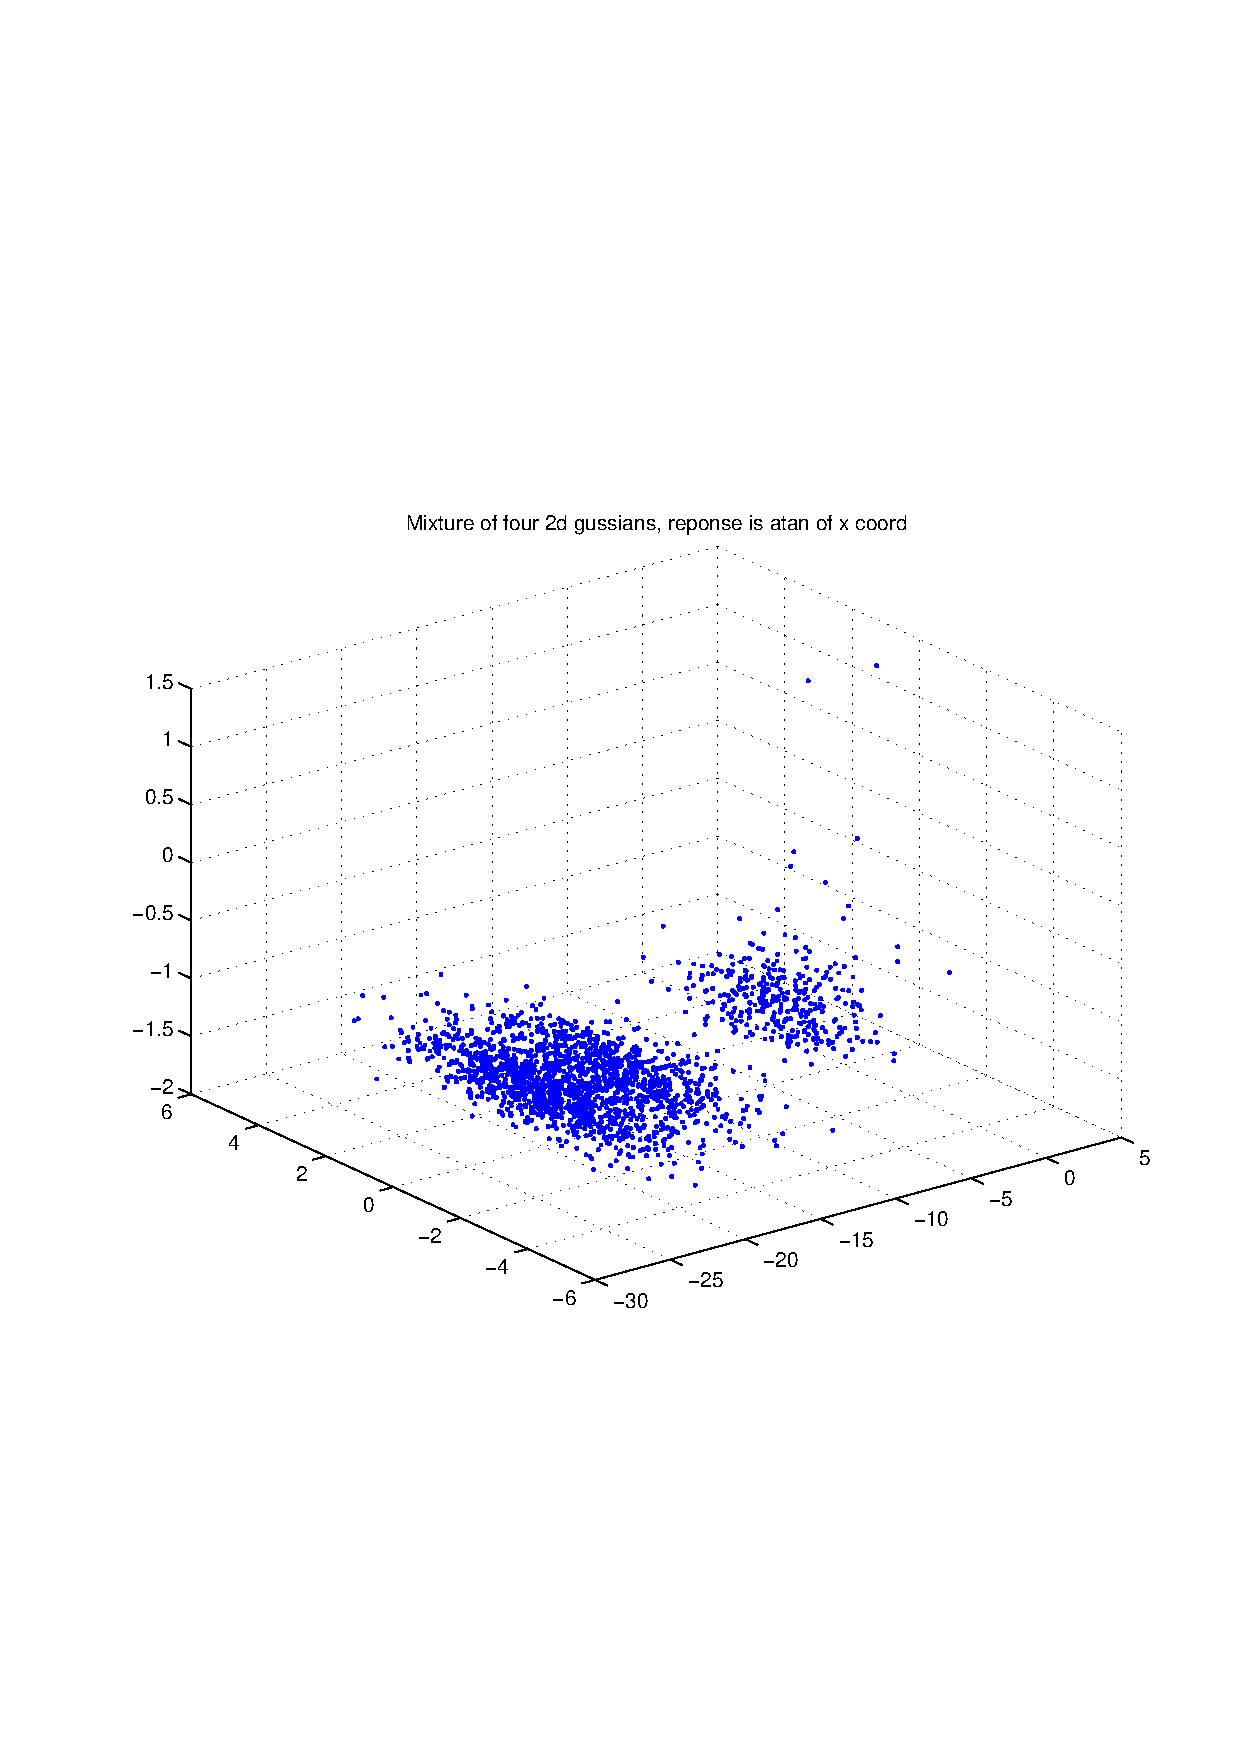
\includegraphics[width=10.0cm,height=10.0cm]{AtanDataSet.pdf}

\subsubsection{3 x 1 Linear Regression}
Sample size = 64

Number of features = 3

$\sigma = \left(
\begin{array}{
ccc}
+3.952 & -0.499 & -0.010 \\
-0.499 & +1.895 & +0.465 \\
-0.010 & +0.465 & +4.477 \\
\end{array}
\right)$ \newline 

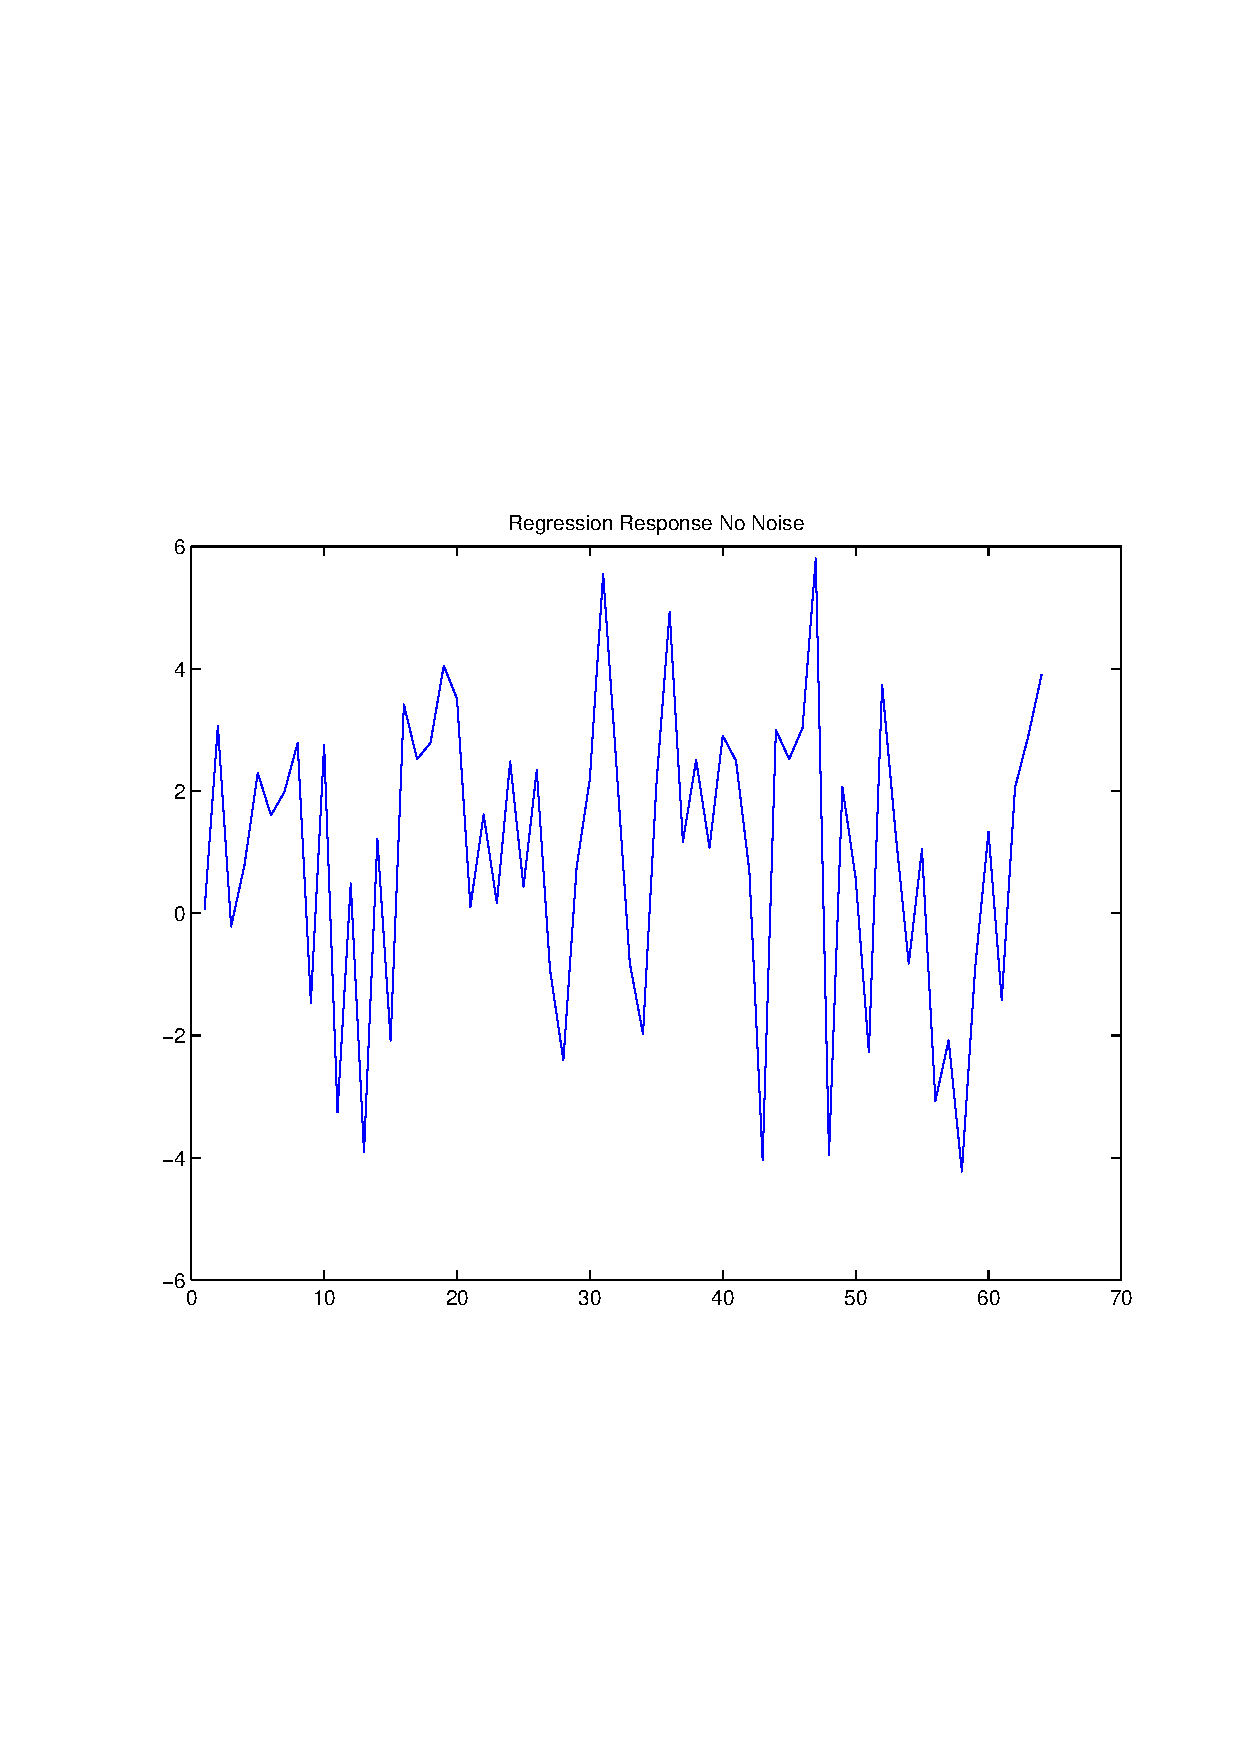
\includegraphics[width=10.0cm,height=10.0cm]{regression_response_no_noise.pdf}

\includegraphics[width=10.0cm,height=10.0cm]{regression_response_with_noise.pdf}

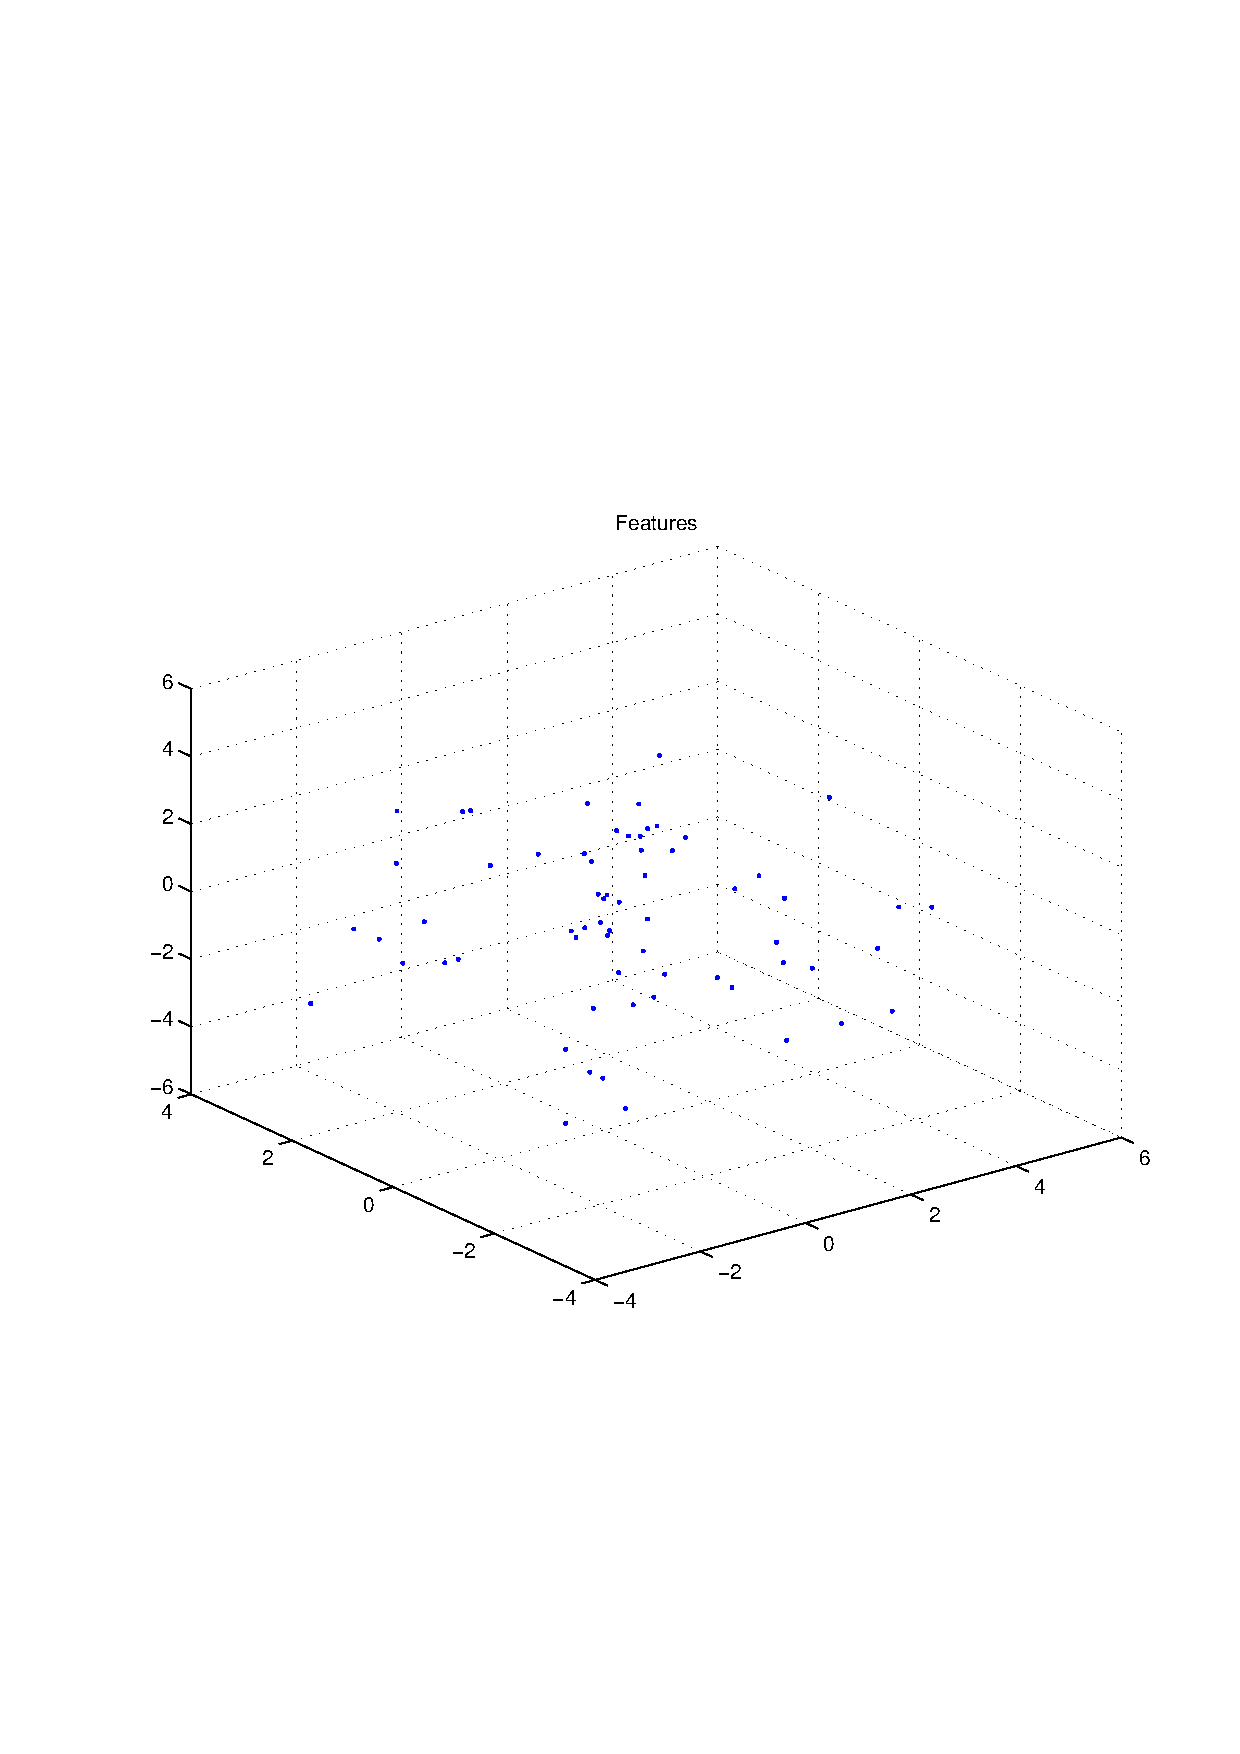
\includegraphics[width=10.0cm,height=10.0cm]{regression_features.pdf}

Beta
+0.817, +0.999, +0.510

Response
-0.275
+3.076
-5.119
+1.252
-4.041
+2.739
+1.813
+2.043
-0.509
+4.198
+2.846
+1.284
-1.095
+0.871
-1.237
+2.107
+0.952
+3.626
-2.933
+6.497
+1.466
+3.319
+3.035
-0.106
+2.350
-1.407
+1.092
-1.334
+2.479
+3.367
+0.327
+2.066
+5.561
-1.237
-6.083
+2.699
-0.197
+1.511
-0.765
-1.252
+0.059
+2.799
-5.335
+1.390
-3.247
+3.563
+0.263
-1.724
+0.719
-1.482
-0.610
-5.399
+1.888
+0.187
+0.476
+2.126
+0.123
+1.530
+0.842
+0.337
-1.658
+0.072
+0.504
-6.061
Estimate for Beta
+0.806
+0.991
+0.511
Error:
-0.011, -0.008, +0.001


QueryPerformanceCounter  =  +4.506
\subsubsection{Fast Gauss Transform}
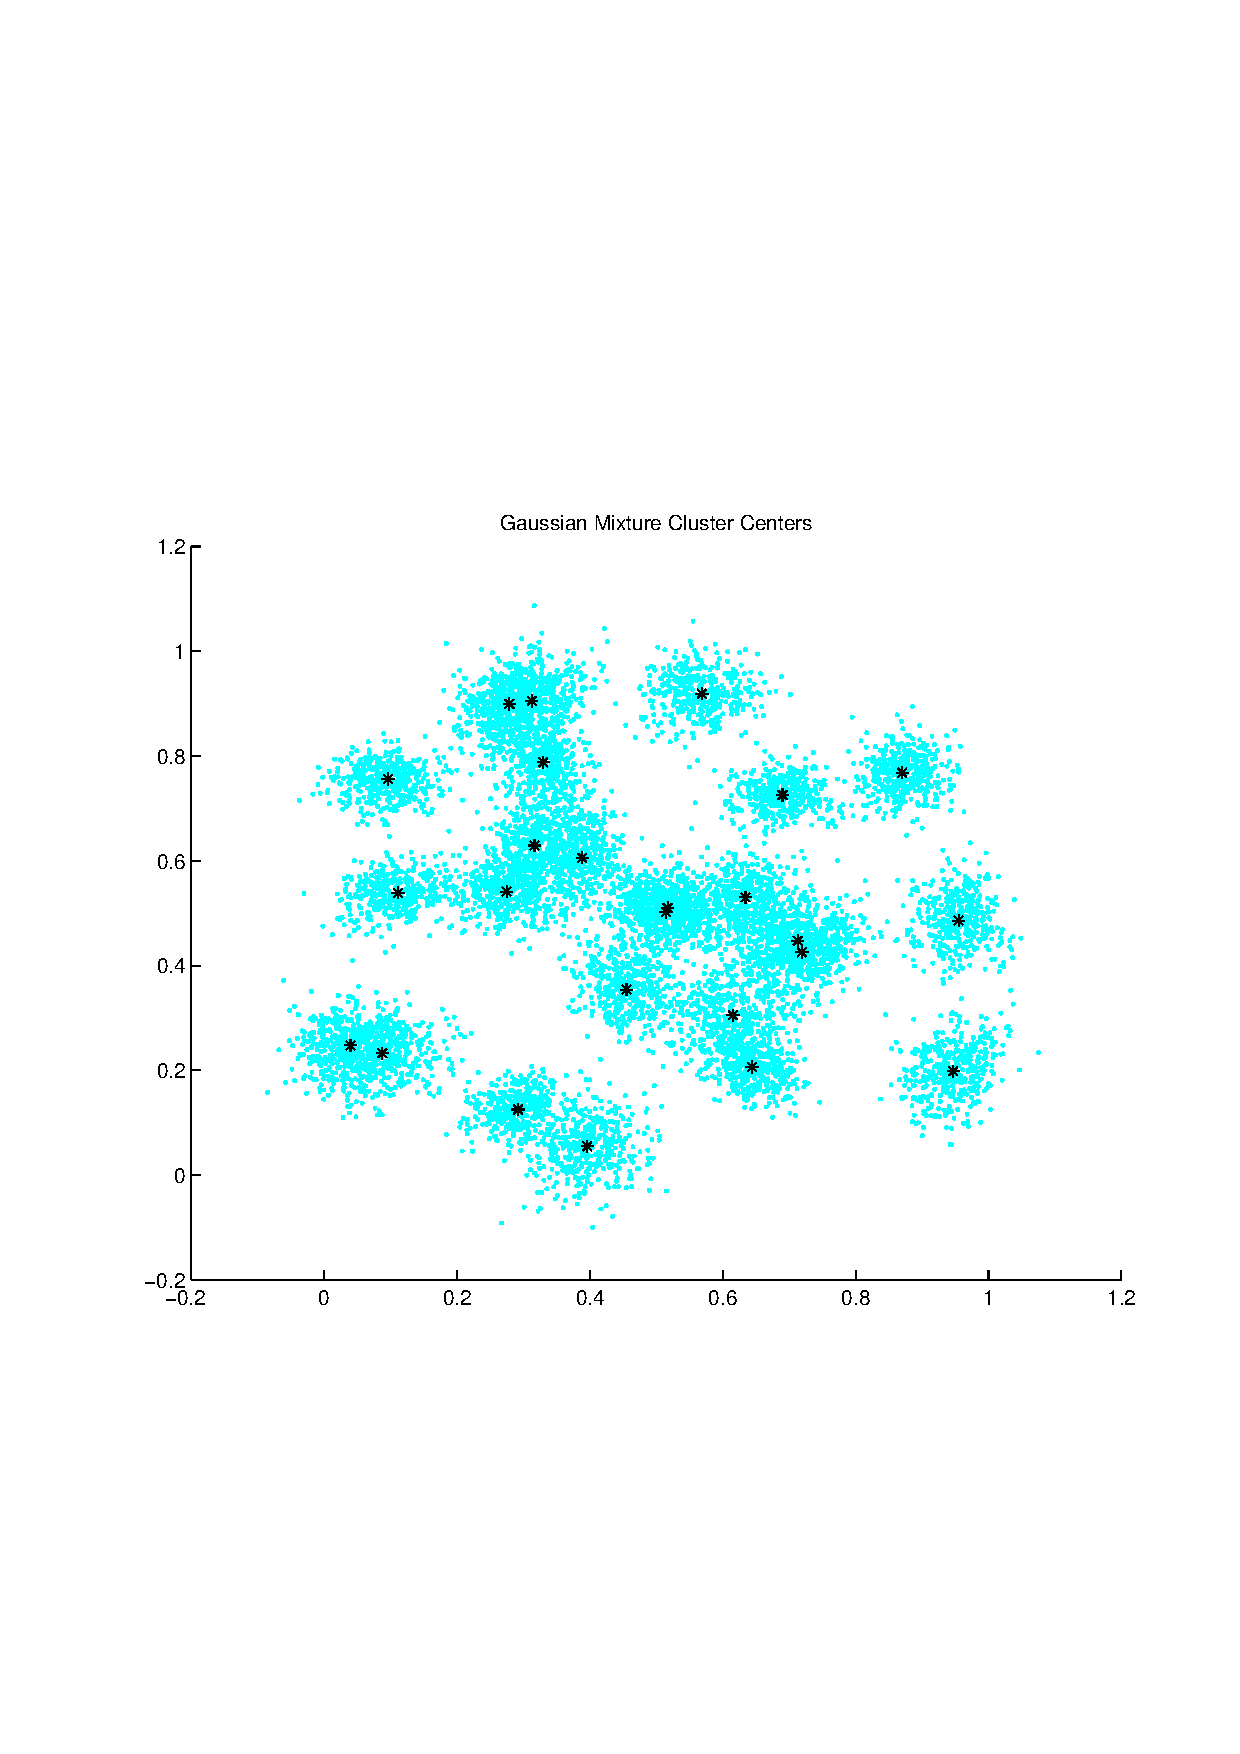
\includegraphics[width=10.0cm,height=10.0cm]{GaussianMixture_ClusterCenters25_Centers.pdf}

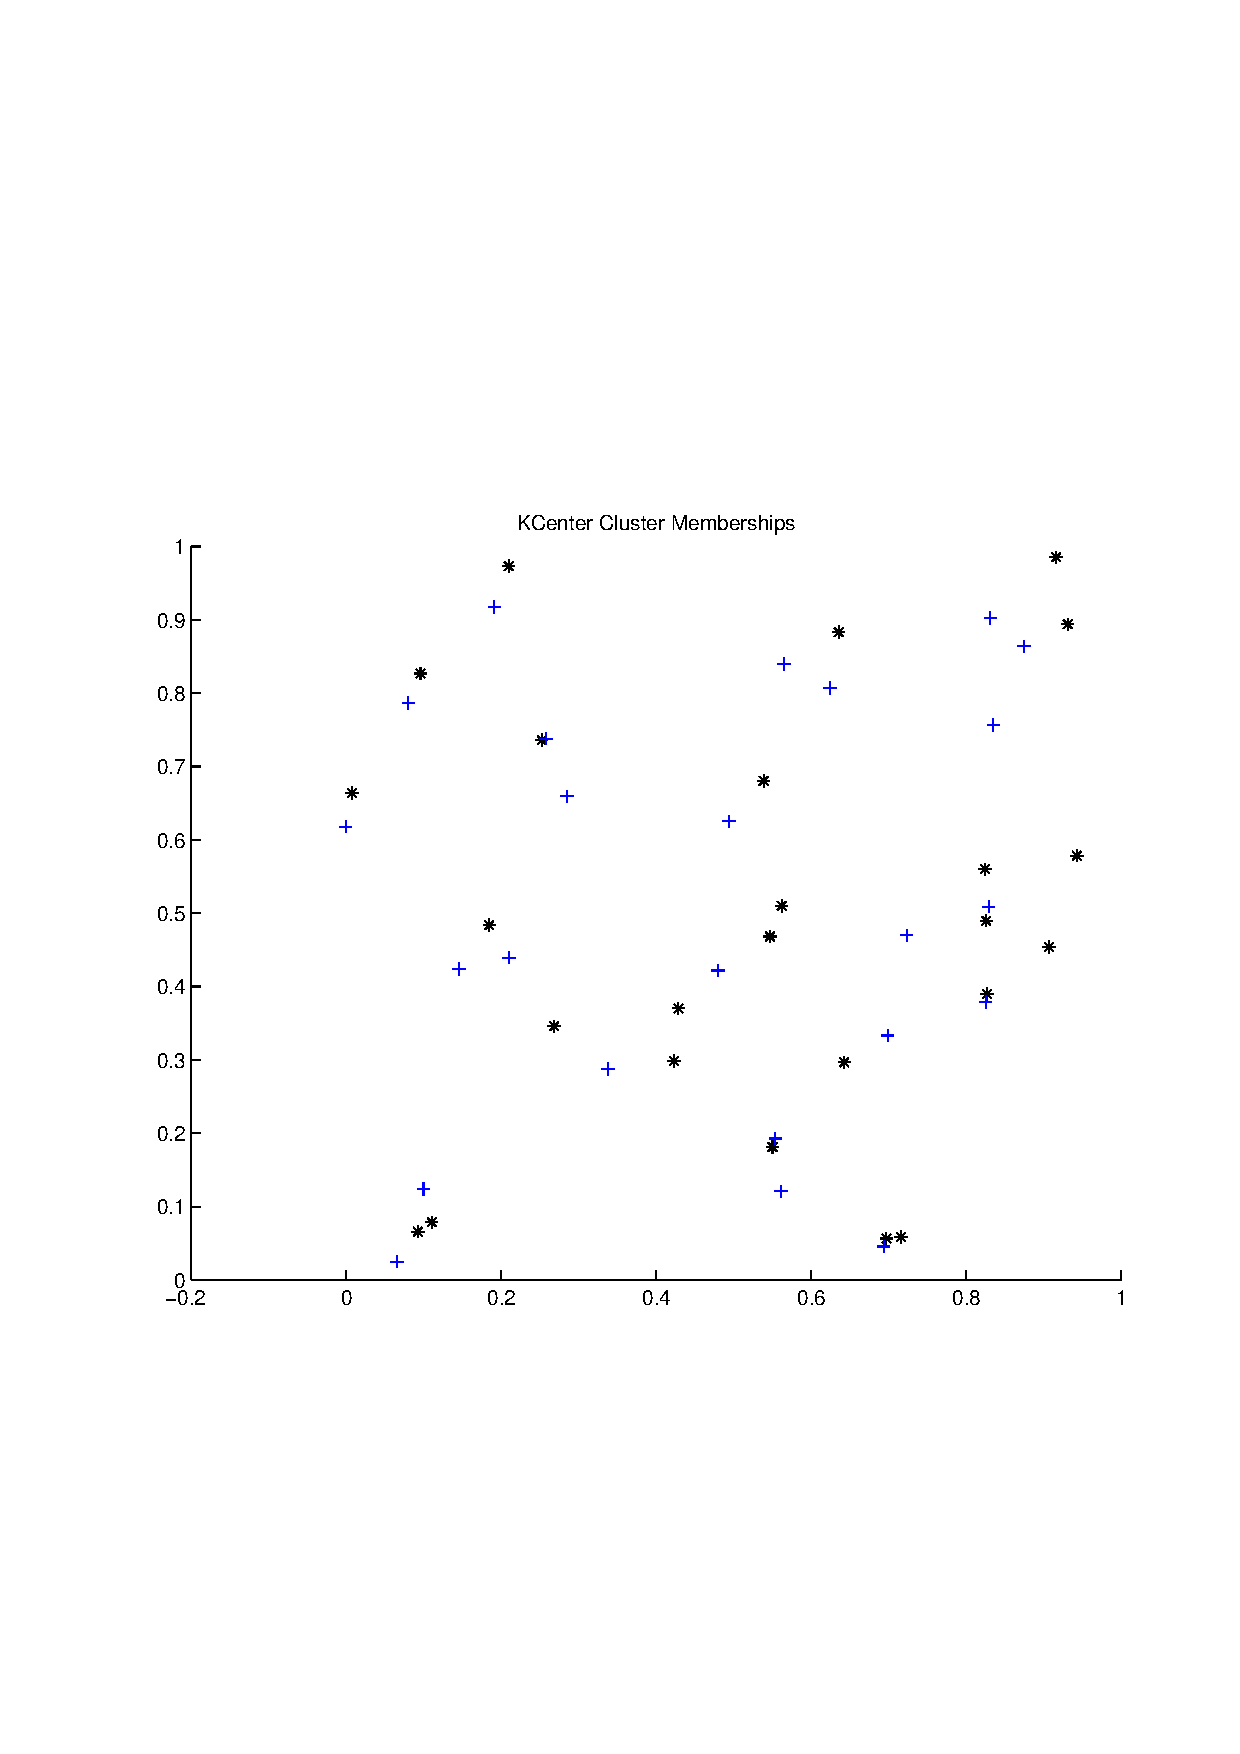
\includegraphics[width=10.0cm,height=10.0cm]{KCenterClusterMemberships_25_Centers.pdf}

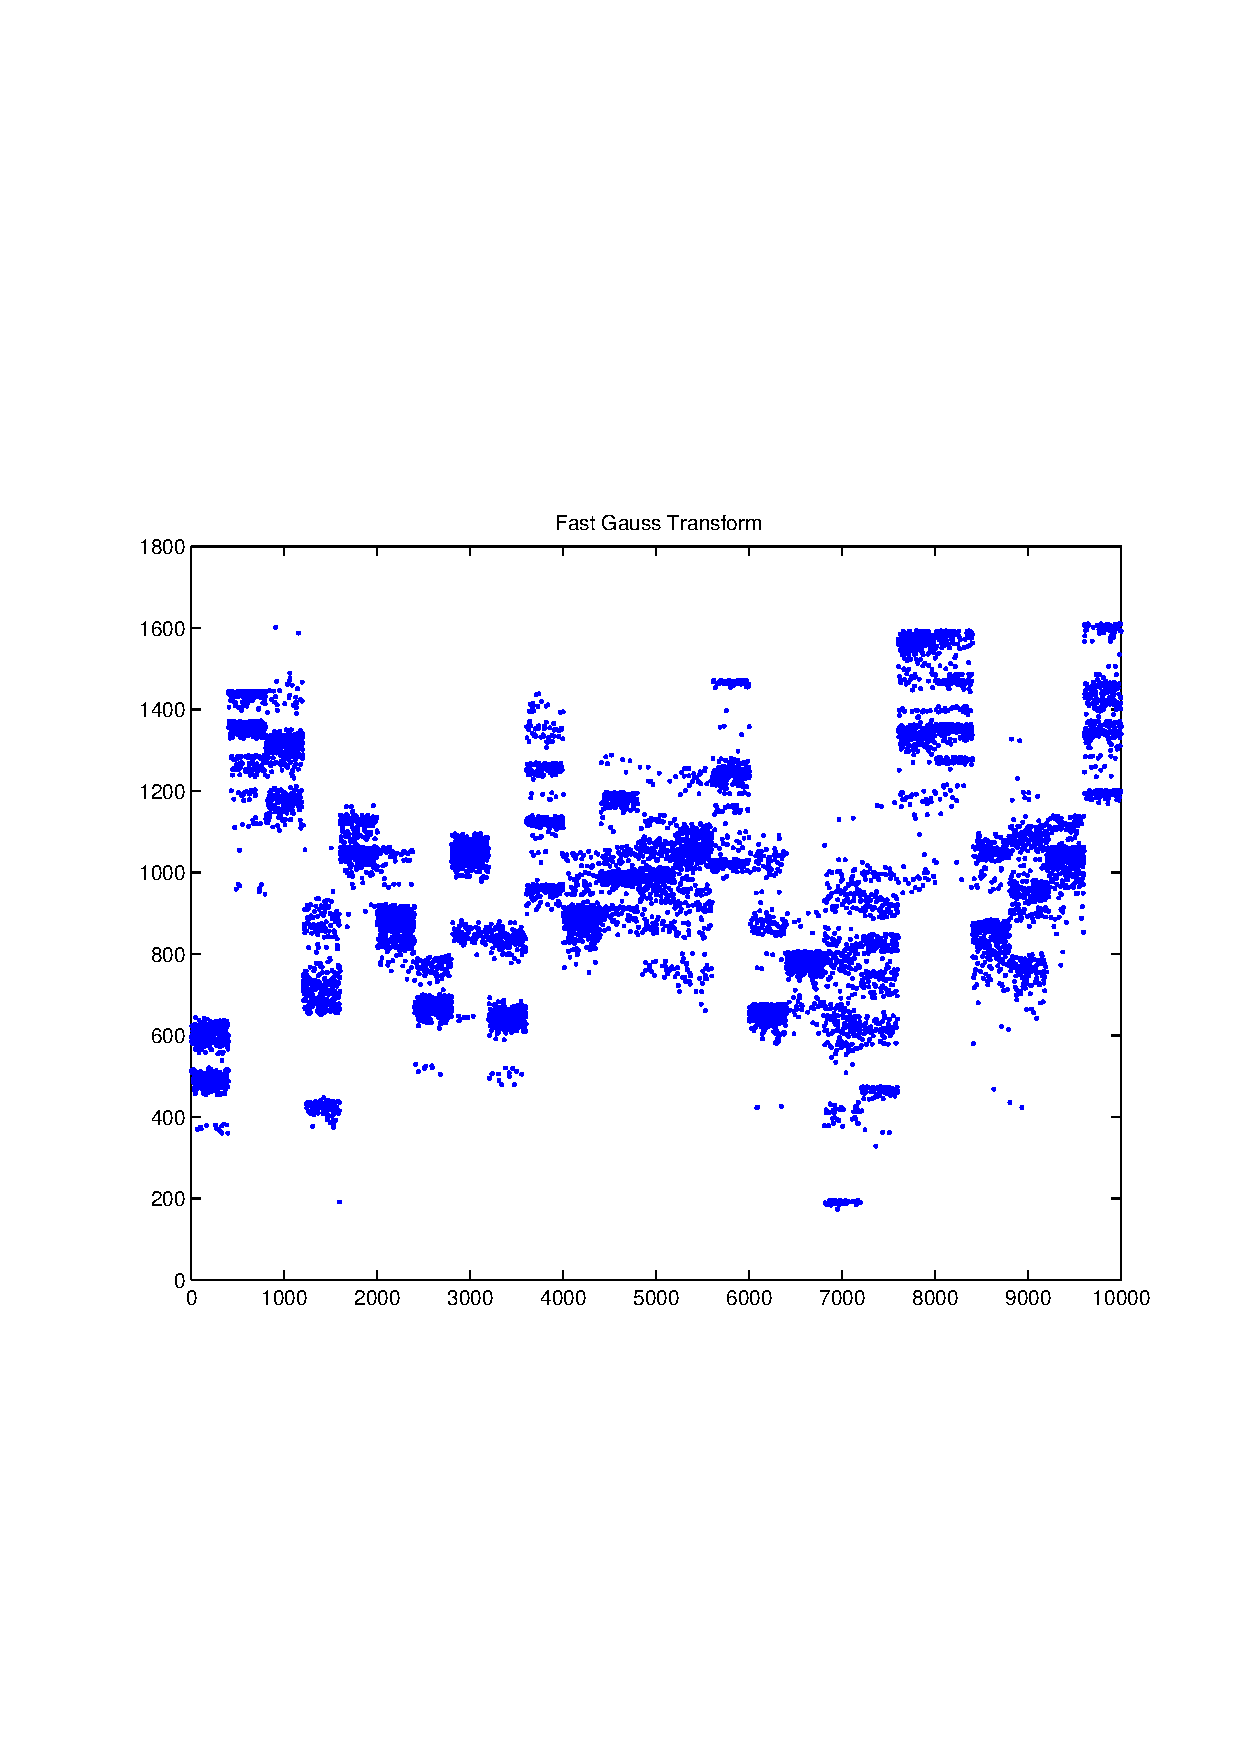
\includegraphics[width=10.0cm,height=10.0cm]{FGT25_Centers.pdf}

QueryPerformanceCounter  =  +6.783
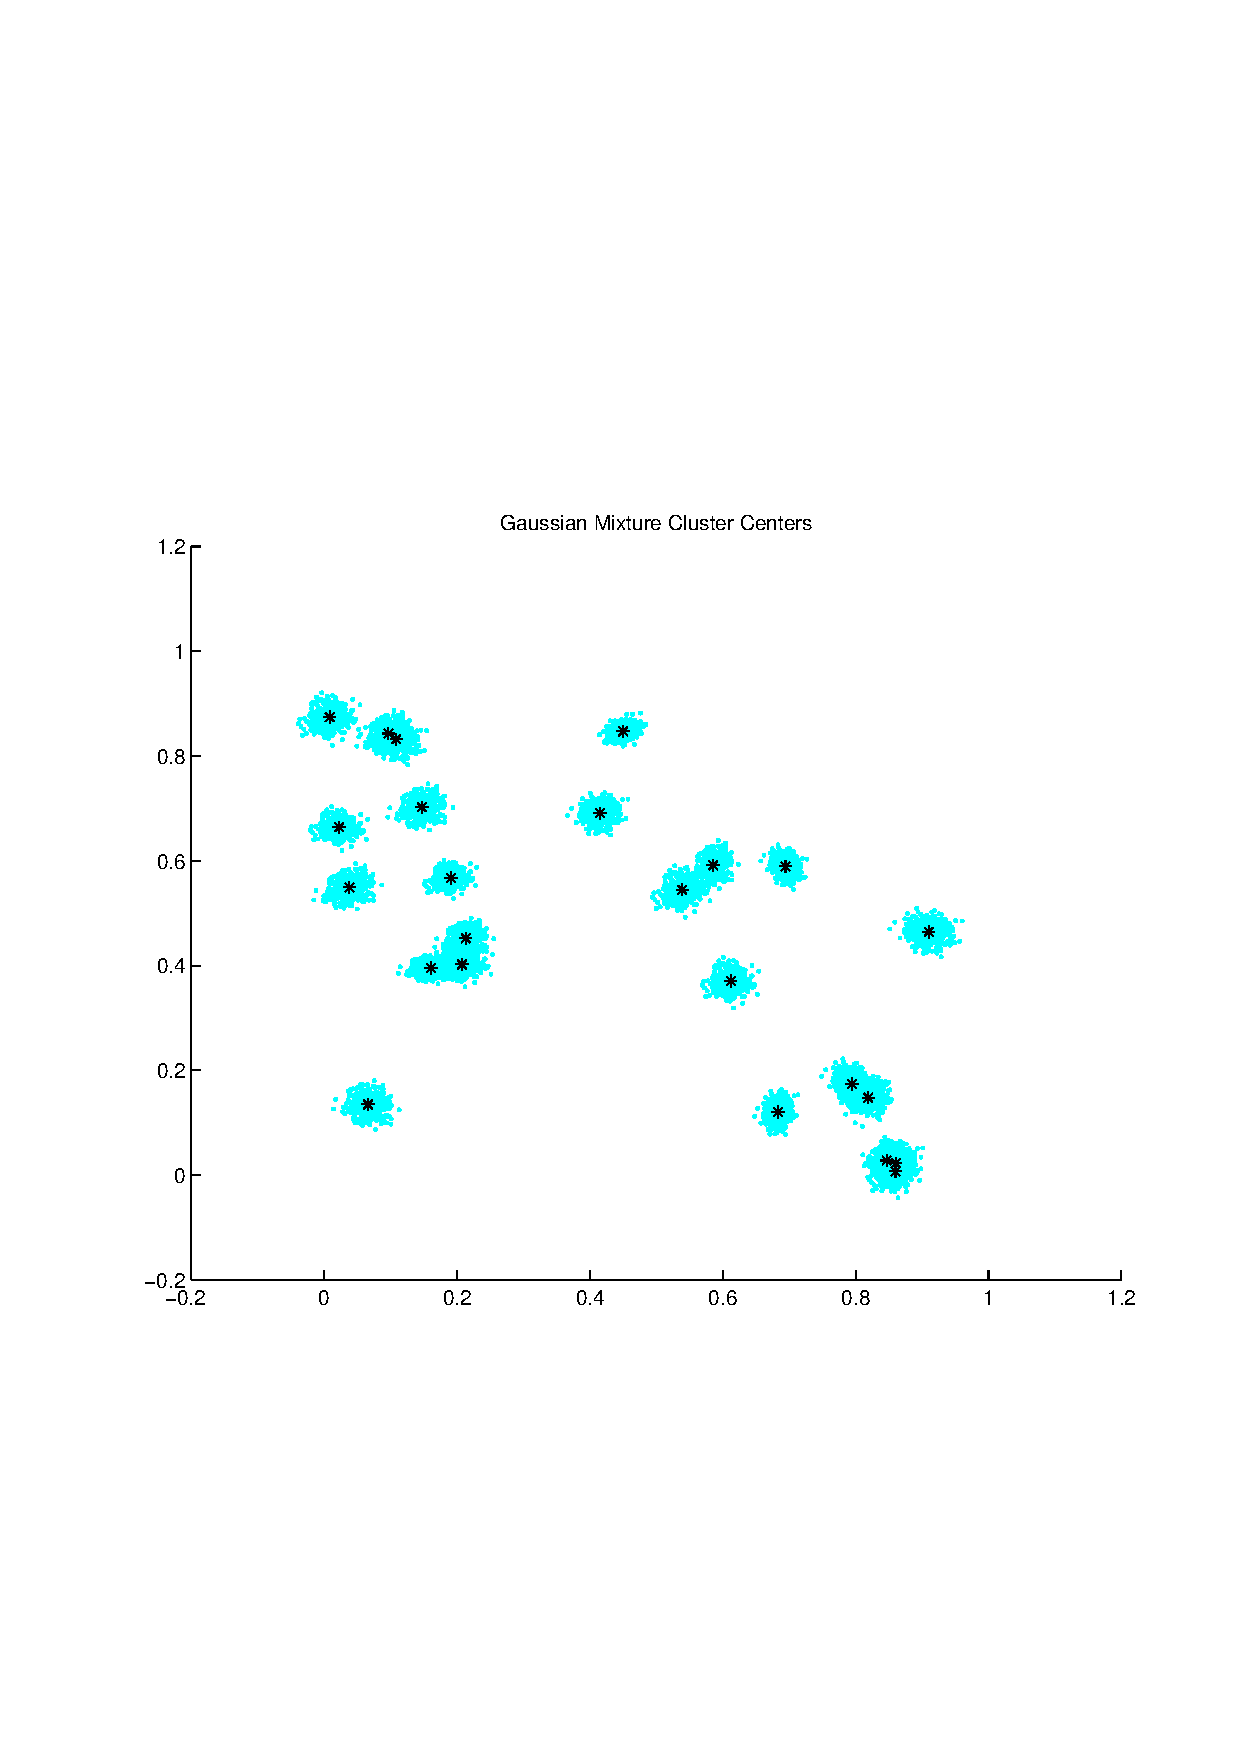
\includegraphics[width=10.0cm,height=10.0cm]{GaussianMixture_ClusterCenters24_Centers.pdf}

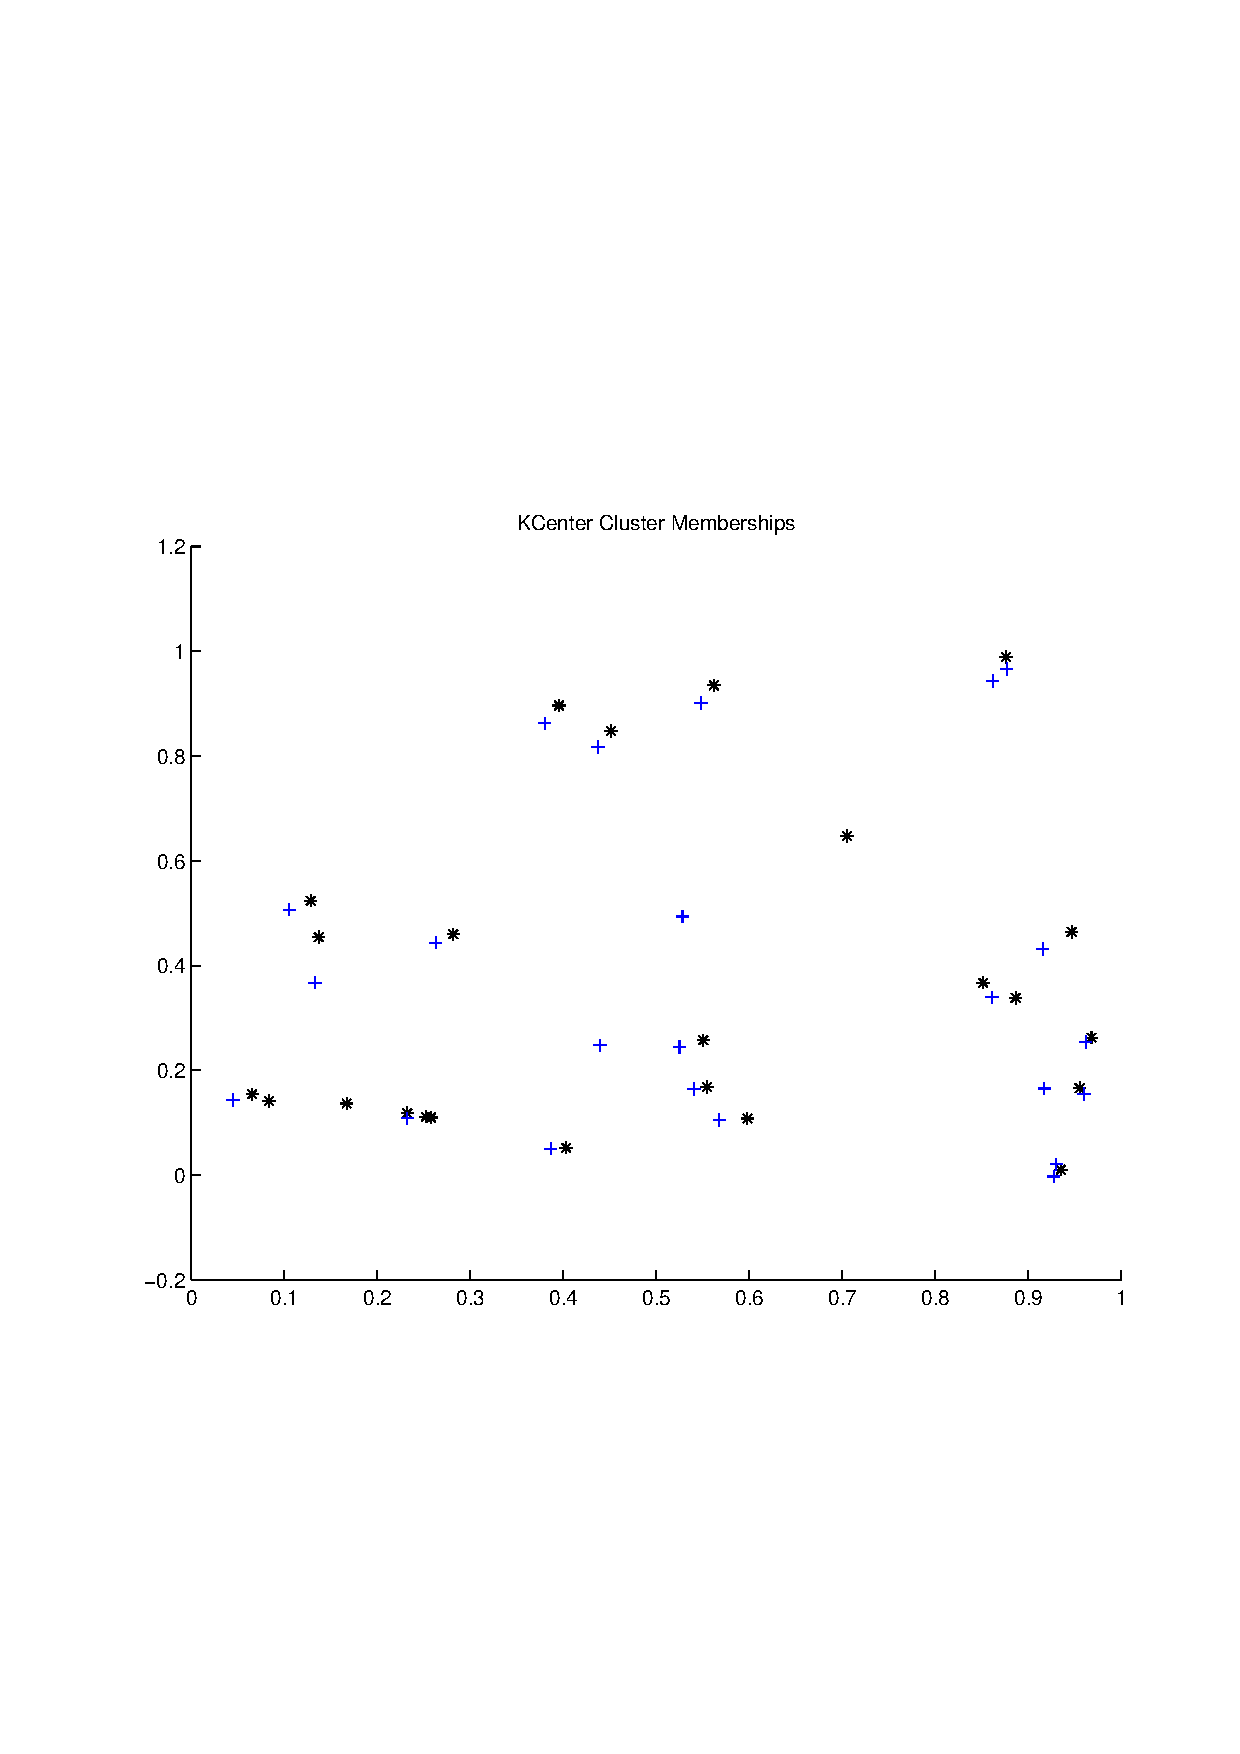
\includegraphics[width=10.0cm,height=10.0cm]{KCenterClusterMemberships_24_Centers.pdf}

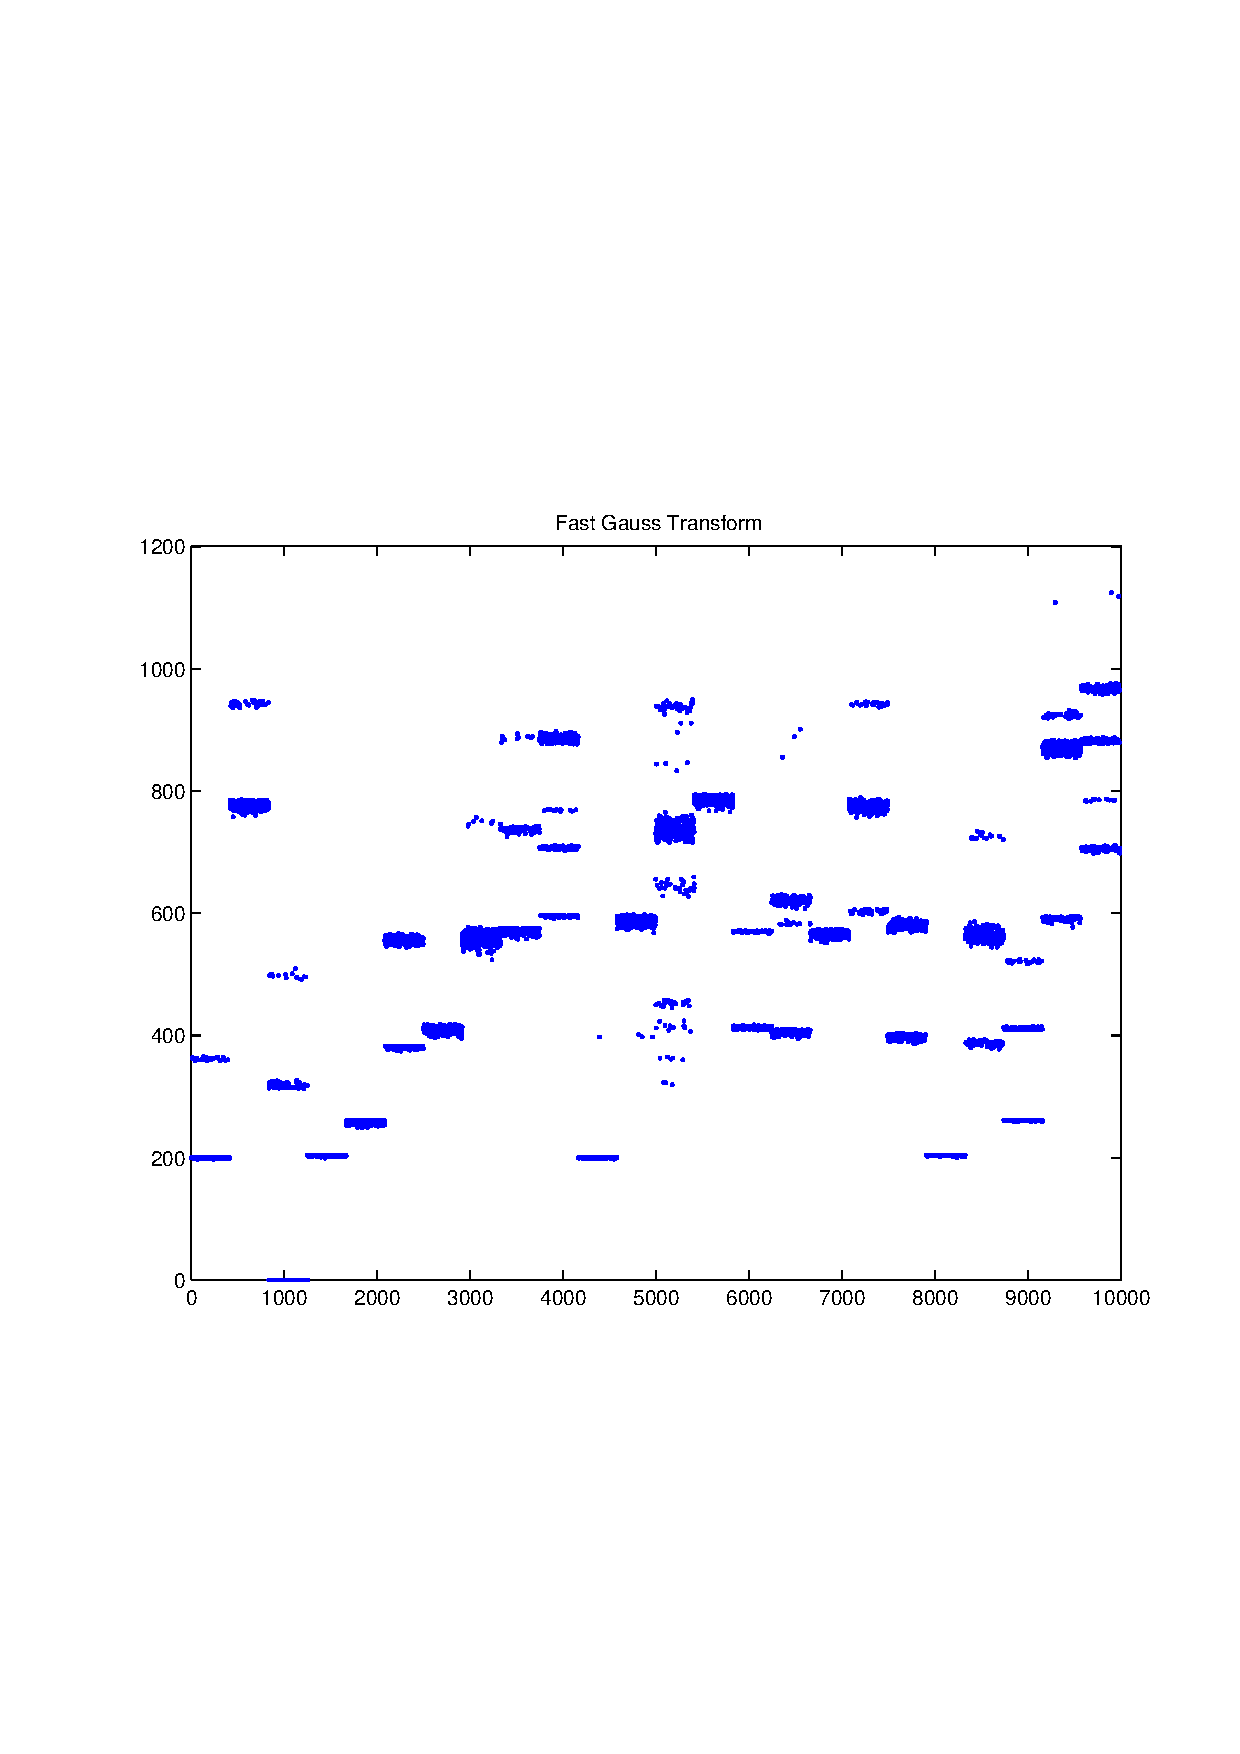
\includegraphics[width=10.0cm,height=10.0cm]{FGT24_Centers.pdf}

QueryPerformanceCounter  =  +8.182
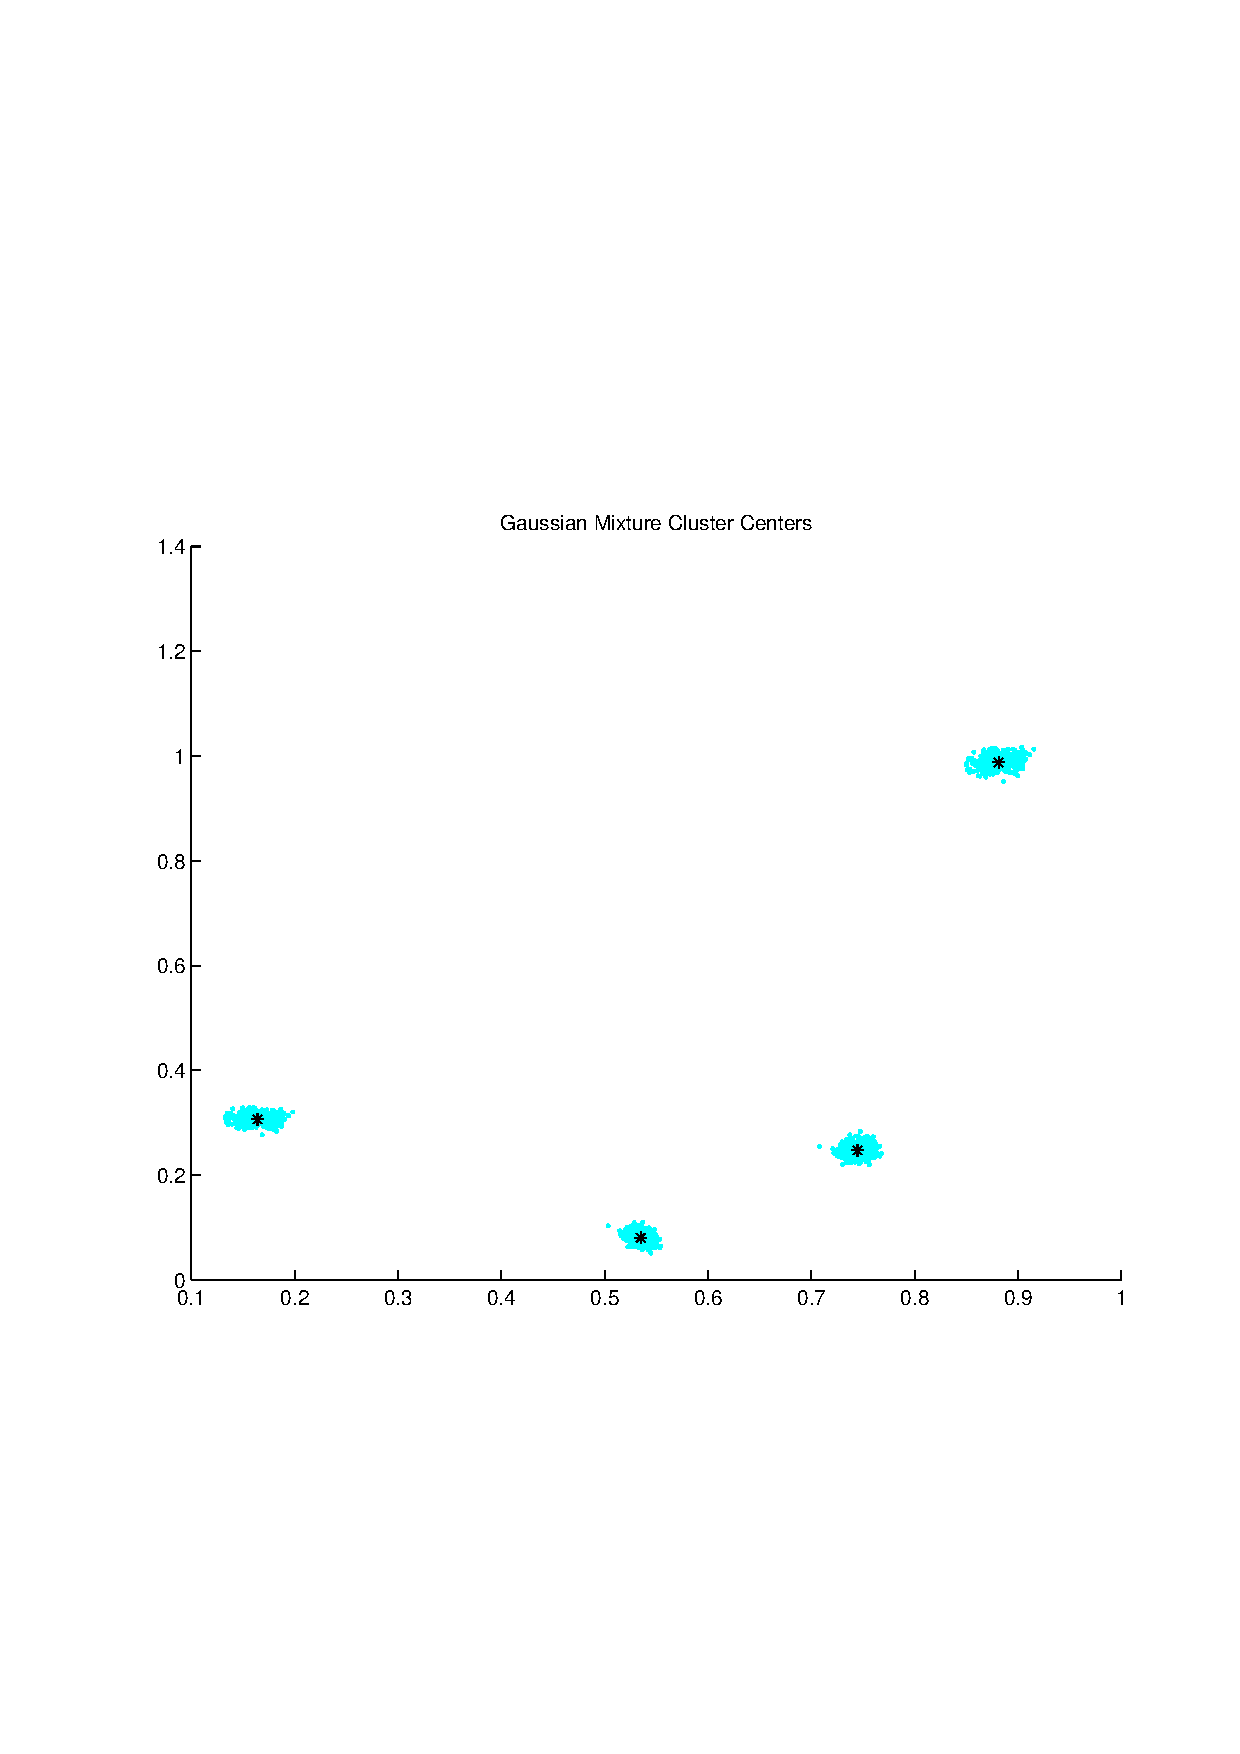
\includegraphics[width=10.0cm,height=10.0cm]{GaussianMixture_ClusterCenters4_Centers.pdf}

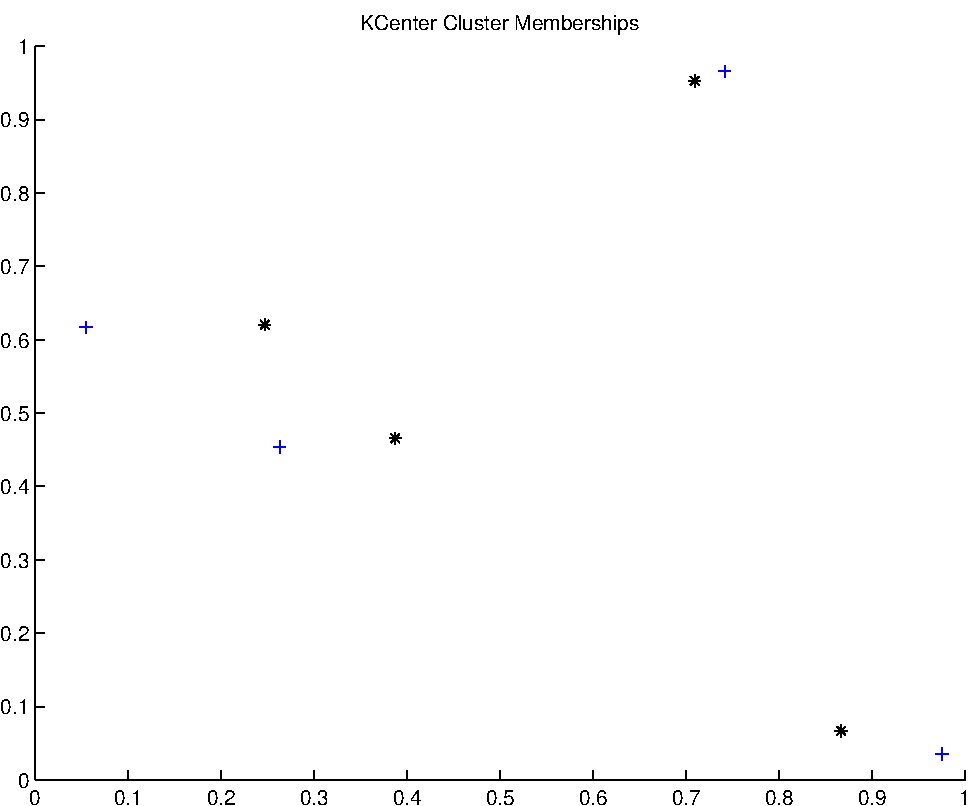
\includegraphics[width=10.0cm,height=10.0cm]{KCenterClusterMemberships_4_Centers.pdf}

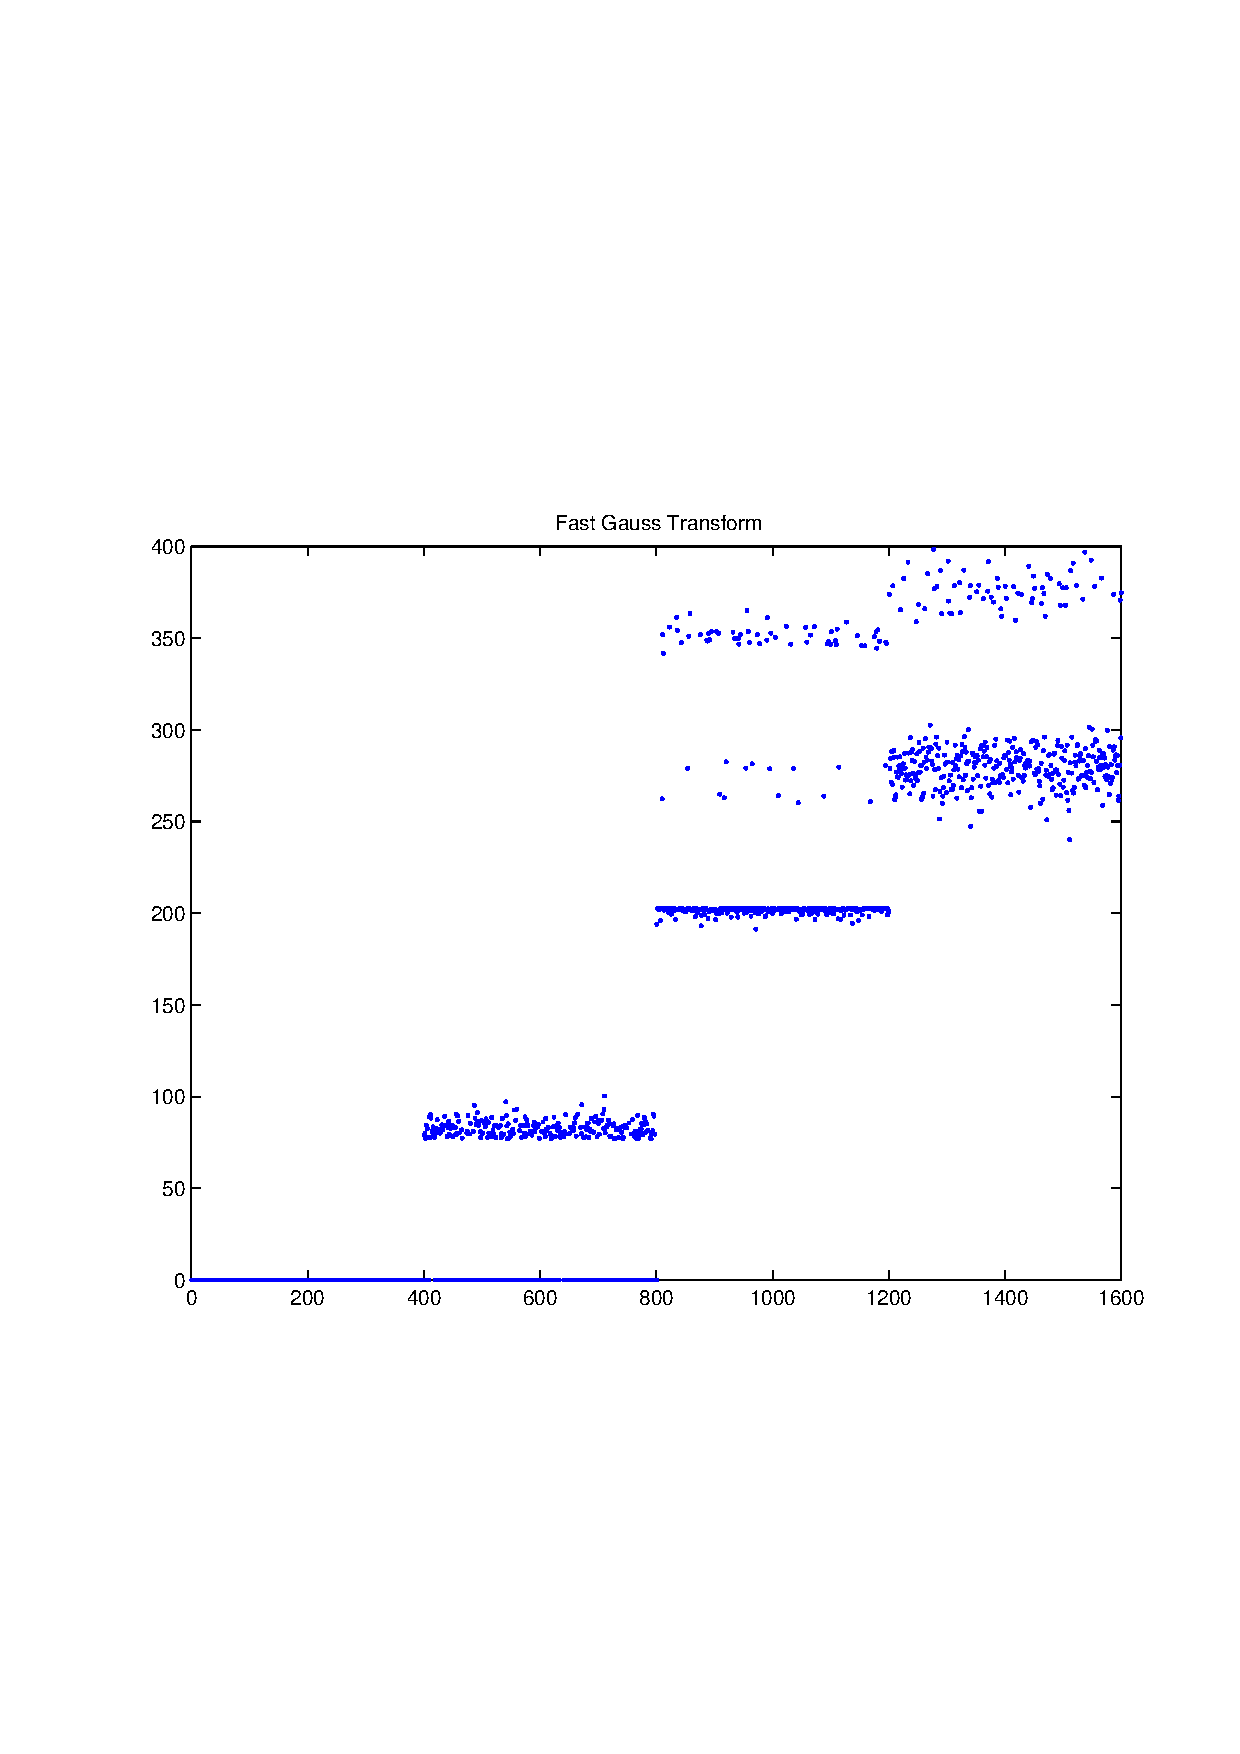
\includegraphics[width=10.0cm,height=10.0cm]{FGT4_Centers.pdf}

QueryPerformanceCounter  =  +3.774
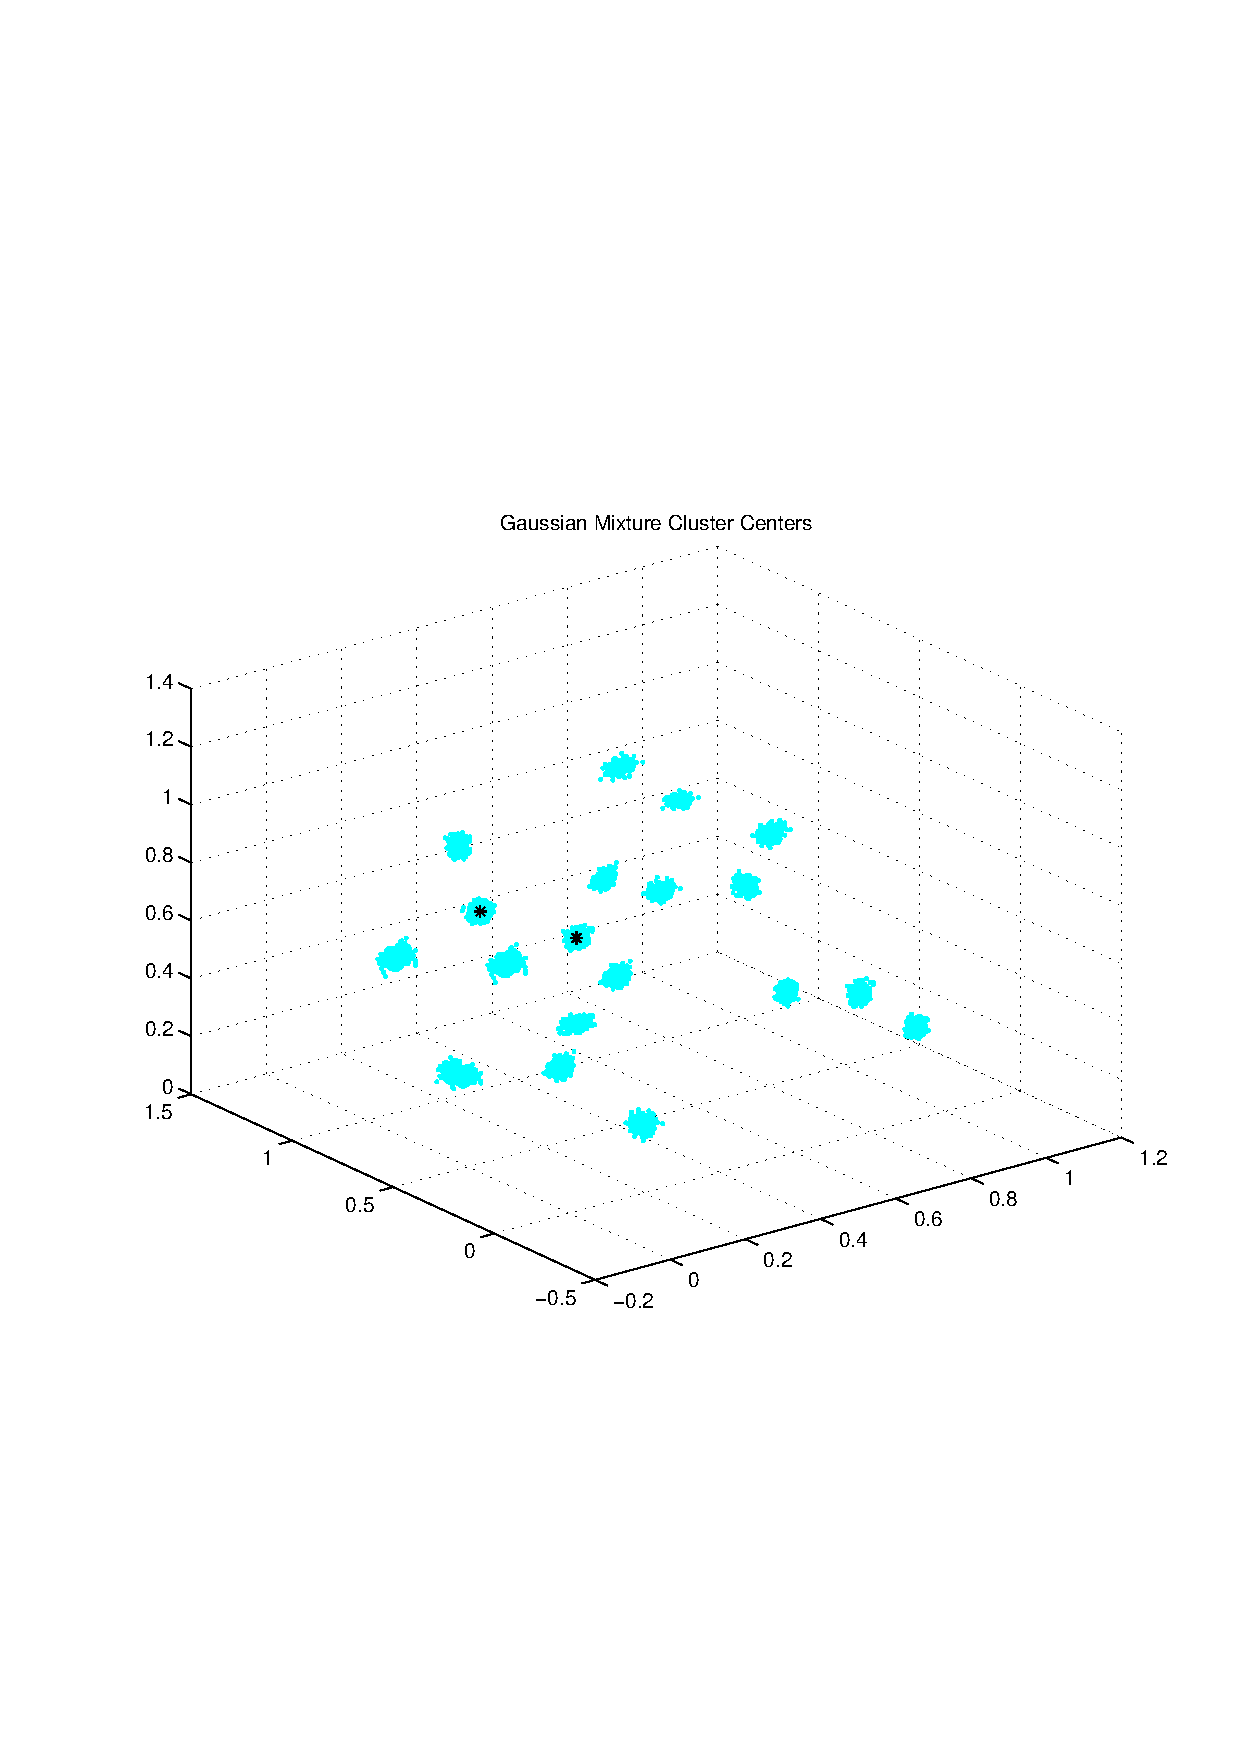
\includegraphics[width=10.0cm,height=10.0cm]{GaussianMixture_ClusterCenters20_Centers.pdf}

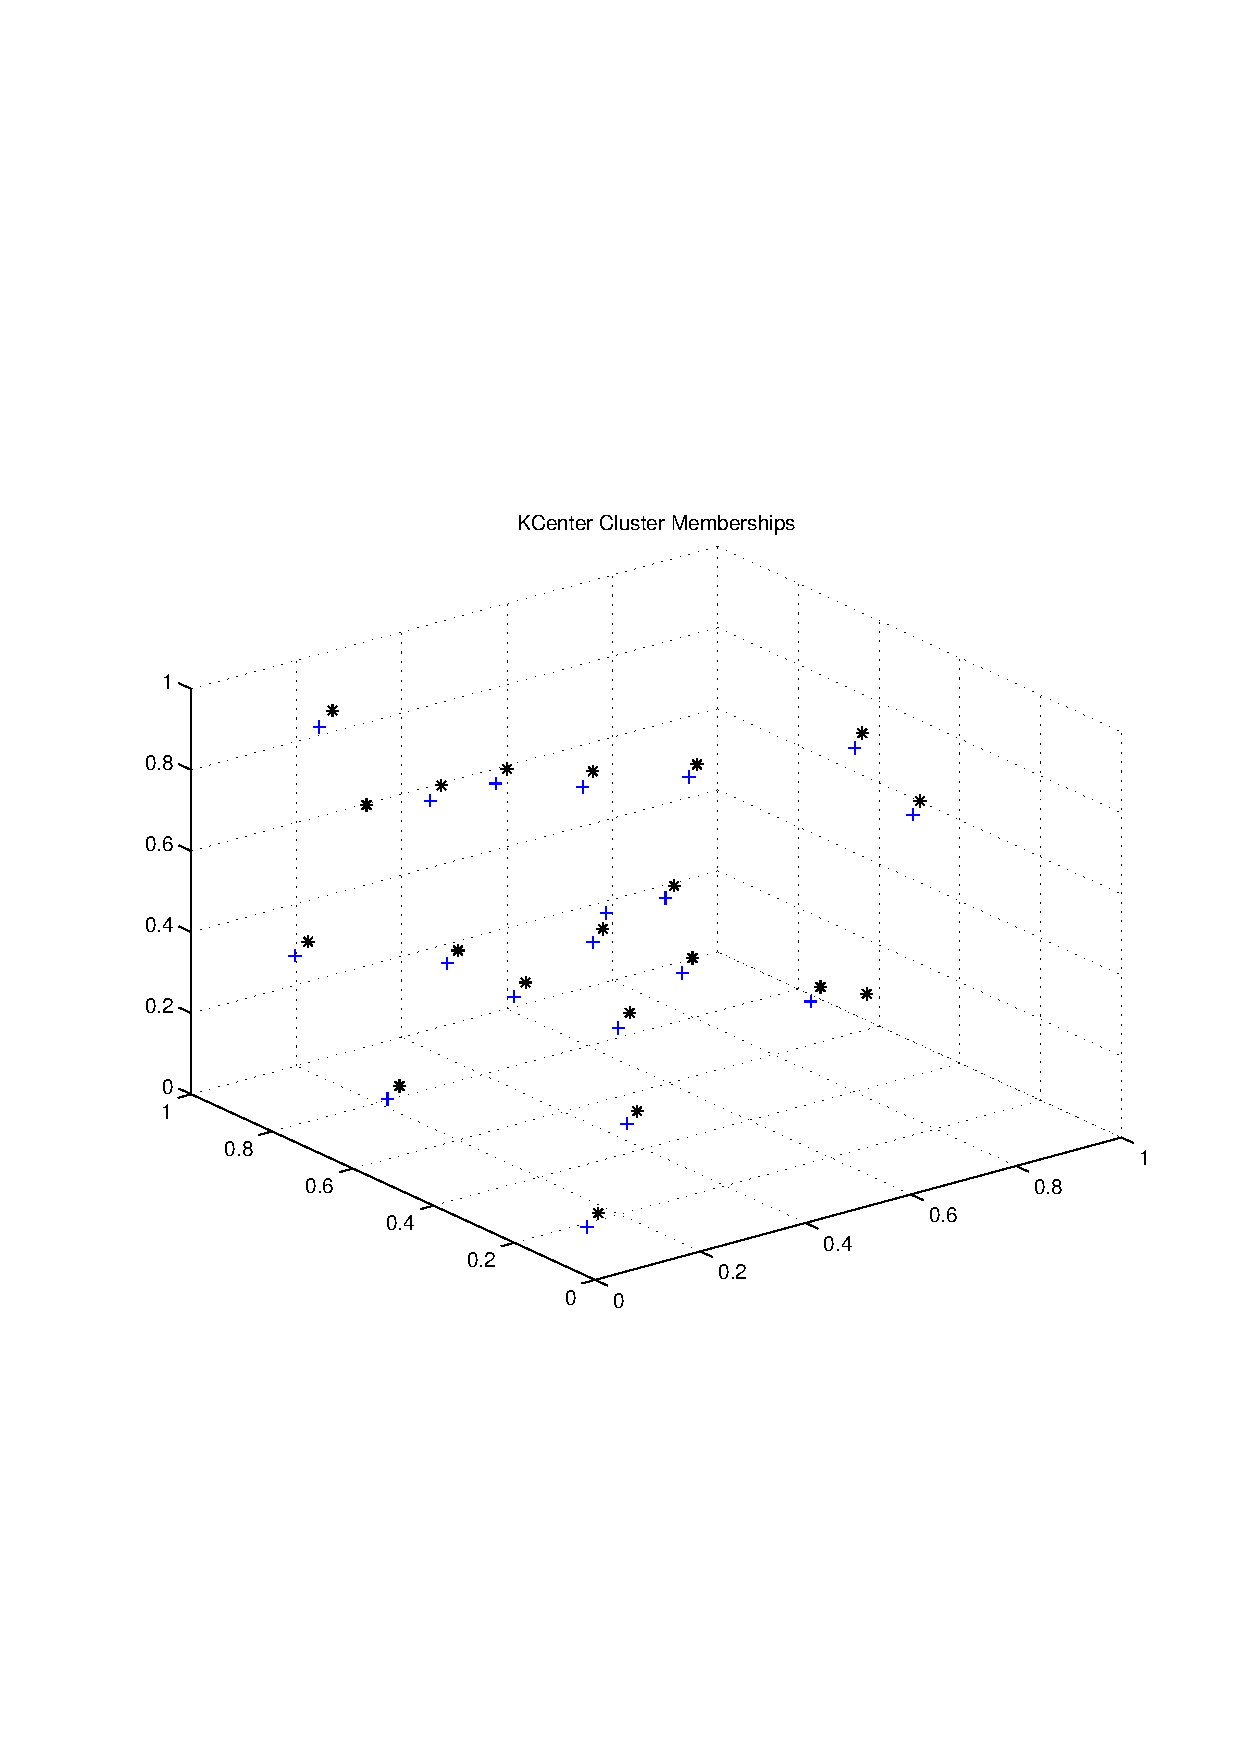
\includegraphics[width=10.0cm,height=10.0cm]{KCenterClusterMemberships_20_Centers.pdf}

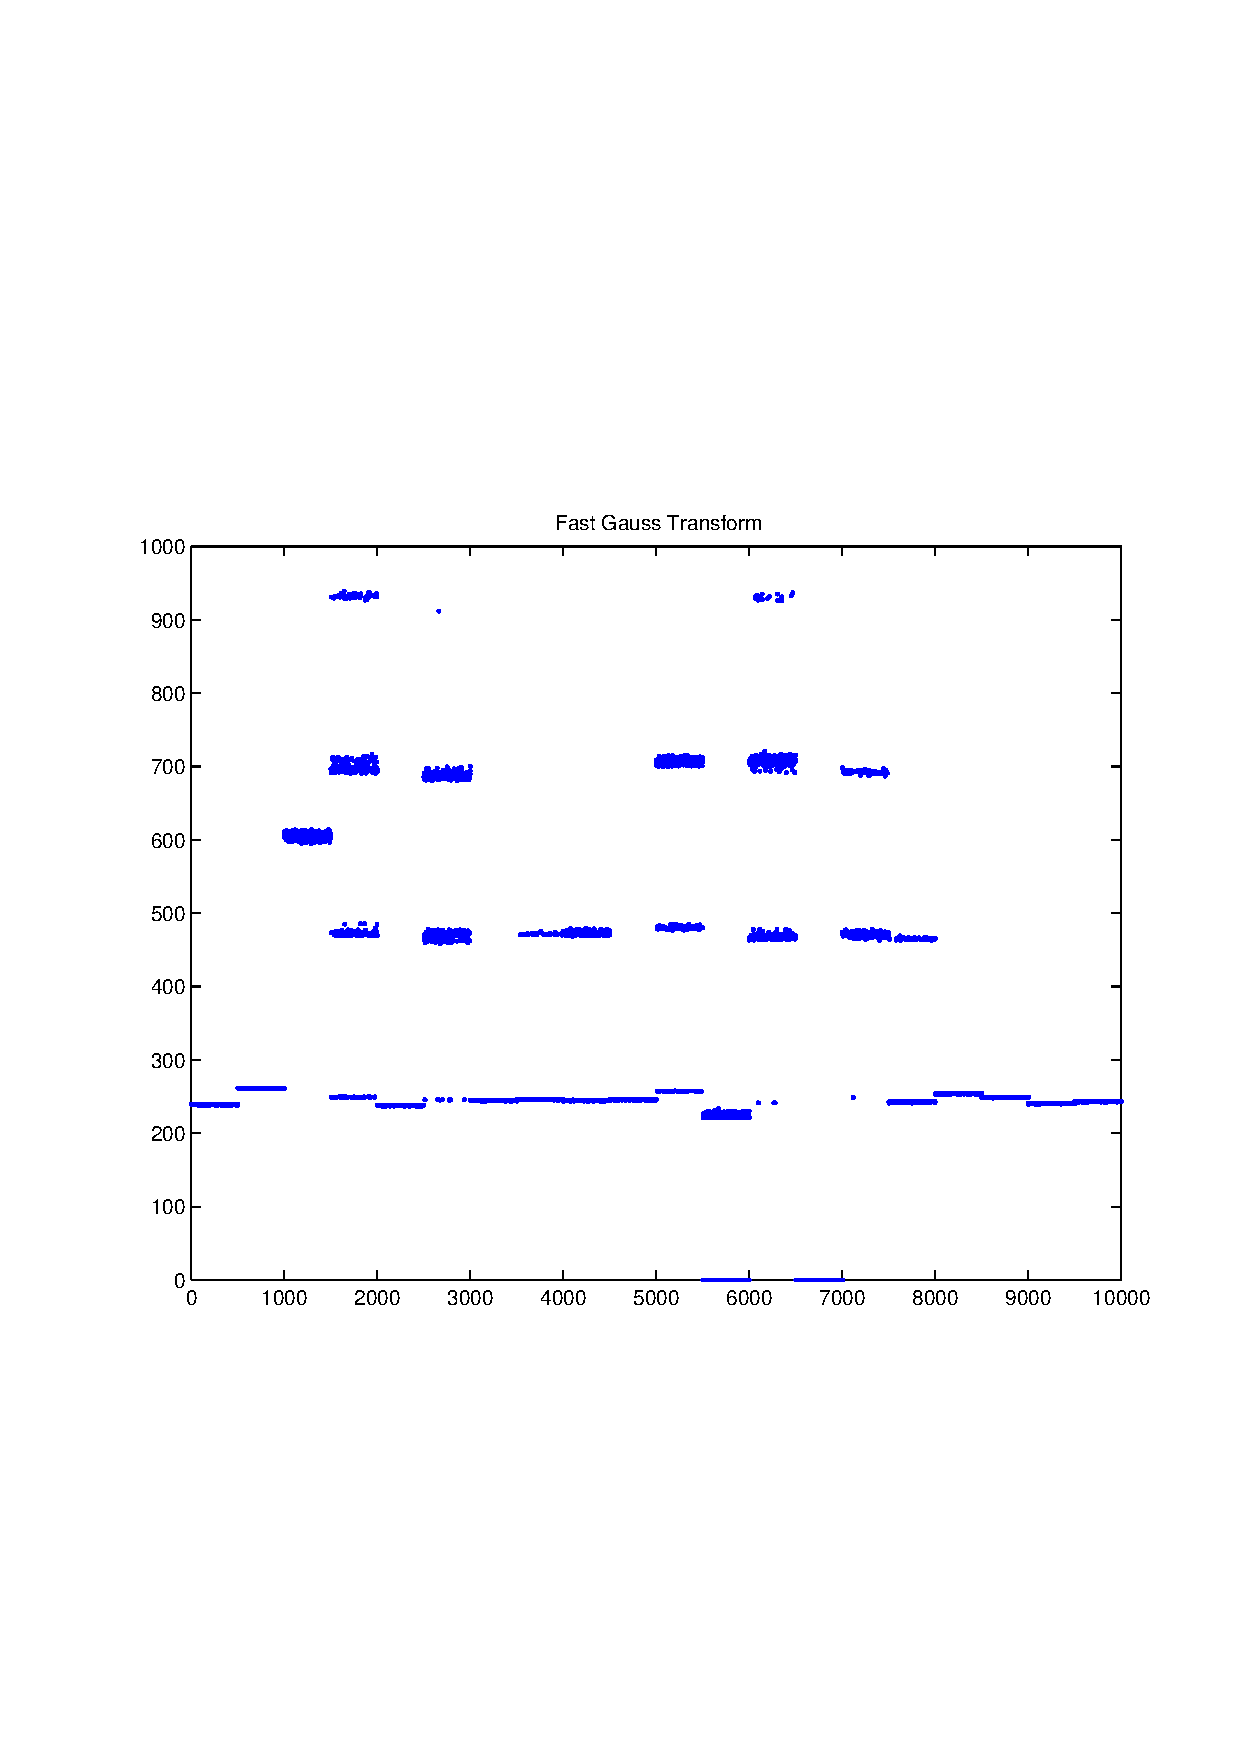
\includegraphics[width=10.0cm,height=10.0cm]{FGT20_Centers.pdf}

QueryPerformanceCounter  =  +6.439
\subsubsection{Matrix Norms}
\subsubsection{Haar Distributed Random Orthogonal Matrix $A \in O(n)$}
 Testing Operator Norm
Number of Dimensions: +12

$A = \left(
\begin{array}{
cccccccccccc}
+0.054 & +0.075 & -0.017 & +0.065 & +0.054 & -0.366 & -0.217 & -0.293 & -0.282 & +0.531 & +0.024 & -0.596 \\
+0.141 & -0.322 & +0.524 & +0.007 & -0.140 & +0.221 & +0.295 & +0.068 & -0.462 & -0.193 & +0.343 & -0.271 \\
+0.025 & -0.173 & -0.455 & -0.429 & -0.041 & -0.130 & +0.526 & +0.439 & +0.028 & +0.212 & +0.052 & -0.208 \\
-0.228 & -0.487 & -0.236 & -0.040 & -0.277 & +0.208 & -0.465 & +0.195 & -0.411 & +0.101 & -0.295 & +0.113 \\
+0.080 & +0.061 & -0.196 & -0.110 & +0.324 & +0.640 & +0.088 & -0.256 & +0.012 & -0.157 & -0.385 & -0.422 \\
-0.216 & -0.174 & +0.153 & +0.428 & +0.006 & +0.034 & +0.546 & -0.165 & -0.033 & +0.416 & -0.402 & +0.232 \\
+0.418 & -0.644 & -0.248 & +0.202 & +0.316 & -0.274 & -0.009 & -0.256 & +0.119 & -0.216 & +0.053 & +0.066 \\
-0.557 & -0.308 & +0.198 & -0.322 & +0.451 & +0.113 & -0.102 & -0.137 & +0.225 & +0.215 & +0.329 & +0.045 \\
+0.267 & +0.032 & +0.082 & +0.390 & +0.411 & +0.243 & -0.193 & +0.620 & +0.081 & +0.318 & +0.105 & -0.029 \\
-0.255 & -0.062 & -0.366 & +0.480 & -0.380 & +0.254 & +0.029 & -0.099 & +0.286 & -0.013 & +0.451 & -0.250 \\
+0.343 & -0.240 & +0.331 & -0.234 & -0.420 & +0.141 & -0.131 & -0.047 & +0.568 & +0.287 & -0.167 & -0.108 \\
-0.365 & -0.131 & +0.223 & +0.183 & +0.037 & -0.339 & -0.035 & +0.324 & +0.247 & -0.390 & -0.359 & -0.449 \\
\end{array}
\right)$ \newline 

$Det(A) :   A \in O(n)$ = (+1.000,+0.000)

$L = \left(
\begin{array}{
cccccccccccc}
+1.000 & +0.000 & +0.000 & +0.000 & +0.000 & +0.000 & +0.000 & +0.000 & +0.000 & +0.000 & +0.000 & +0.000 \\
-0.752 & +1.000 & +0.000 & +0.000 & +0.000 & +0.000 & +0.000 & +0.000 & +0.000 & +0.000 & +0.000 & +0.000 \\
-0.254 & +0.457 & +1.000 & +0.000 & +0.000 & +0.000 & +0.000 & +0.000 & +0.000 & +0.000 & +0.000 & +0.000 \\
+0.458 & -0.091 & -0.751 & +1.000 & +0.000 & +0.000 & +0.000 & +0.000 & +0.000 & +0.000 & +0.000 & +0.000 \\
-0.044 & +0.214 & -0.685 & -0.812 & +1.000 & +0.000 & +0.000 & +0.000 & +0.000 & +0.000 & +0.000 & +0.000 \\
-0.144 & -0.019 & -0.274 & -0.296 & -0.083 & +1.000 & +0.000 & +0.000 & +0.000 & +0.000 & +0.000 & +0.000 \\
+0.409 & +0.412 & -0.447 & +0.142 & +0.760 & -0.059 & +1.000 & +0.000 & +0.000 & +0.000 & +0.000 & +0.000 \\
-0.479 & +0.132 & +0.307 & +0.445 & -0.973 & +0.559 & -0.318 & +1.000 & +0.000 & +0.000 & +0.000 & +0.000 \\
-0.616 & +0.491 & +0.810 & -0.631 & +0.680 & -0.037 & +0.852 & -0.391 & +1.000 & +0.000 & +0.000 & +0.000 \\
-0.098 & -0.051 & -0.004 & +0.053 & -0.170 & -0.329 & -0.030 & -0.205 & -0.285 & +1.000 & +0.000 & +0.000 \\
+0.388 & +0.062 & +0.133 & +0.967 & -0.573 & -0.195 & -0.869 & +0.098 & -0.381 & +0.853 & +1.000 & +0.000 \\
+0.657 & -0.081 & +0.136 & +0.685 & -0.362 & -0.647 & -0.341 & +0.351 & -0.059 & -0.885 & +0.517 & +1.000 \\
\end{array}
\right)$ \newline 

$U = \left(
\begin{array}{
cccccccccccc}
-0.557 & -0.308 & +0.198 & -0.322 & +0.451 & +0.113 & -0.102 & -0.137 & +0.225 & +0.215 & +0.329 & +0.045 \\
+0.000 & -0.876 & -0.099 & -0.040 & +0.655 & -0.189 & -0.086 & -0.359 & +0.287 & -0.054 & +0.300 & +0.100 \\
+0.000 & +0.000 & +0.620 & -0.056 & -0.325 & +0.336 & +0.309 & +0.198 & -0.536 & -0.113 & +0.289 & -0.305 \\
+0.000 & +0.000 & +0.000 & +0.582 & -0.771 & +0.438 & +0.300 & +0.080 & -0.194 & -0.202 & +0.545 & -0.491 \\
+0.000 & +0.000 & +0.000 & +0.000 & -1.010 & +0.502 & +0.996 & +0.710 & -0.548 & -0.009 & +0.643 & -0.835 \\
+0.000 & +0.000 & +0.000 & +0.000 & +0.000 & +0.916 & +0.328 & -0.146 & -0.200 & -0.219 & -0.038 & -0.712 \\
+0.000 & +0.000 & +0.000 & +0.000 & +0.000 & +0.000 & -1.029 & -0.072 & -0.429 & +0.007 & -0.992 & +0.579 \\
+0.000 & +0.000 & +0.000 & +0.000 & +0.000 & +0.000 & +0.000 & +1.256 & -0.157 & +0.668 & +0.223 & +0.061 \\
+0.000 & +0.000 & +0.000 & +0.000 & +0.000 & +0.000 & +0.000 & +0.000 & +1.547 & +0.664 & +0.492 & -0.121 \\
+0.000 & +0.000 & +0.000 & +0.000 & +0.000 & +0.000 & +0.000 & +0.000 & +0.000 & +0.813 & +0.297 & -0.942 \\
+0.000 & +0.000 & +0.000 & +0.000 & +0.000 & +0.000 & +0.000 & +0.000 & +0.000 & +0.000 & -1.702 & +1.361 \\
+0.000 & +0.000 & +0.000 & +0.000 & +0.000 & +0.000 & +0.000 & +0.000 & +0.000 & +0.000 & +0.000 & -2.225 \\
\end{array}
\right)$ \newline 

$L * U  = \left(
\begin{array}{
cccccccccccc}
-0.557 & -0.308 & +0.198 & -0.322 & +0.451 & +0.113 & -0.102 & -0.137 & +0.225 & +0.215 & +0.329 & +0.045 \\
+0.418 & -0.644 & -0.248 & +0.202 & +0.316 & -0.274 & -0.009 & -0.256 & +0.119 & -0.216 & +0.053 & +0.066 \\
+0.141 & -0.322 & +0.524 & +0.007 & -0.140 & +0.221 & +0.295 & +0.068 & -0.462 & -0.193 & +0.343 & -0.271 \\
-0.255 & -0.062 & -0.366 & +0.480 & -0.380 & +0.254 & +0.029 & -0.099 & +0.286 & -0.013 & +0.451 & -0.250 \\
+0.025 & -0.173 & -0.455 & -0.429 & -0.041 & -0.130 & +0.526 & +0.439 & +0.028 & +0.212 & +0.052 & -0.208 \\
+0.080 & +0.061 & -0.196 & -0.110 & +0.324 & +0.640 & +0.088 & -0.256 & +0.012 & -0.157 & -0.385 & -0.422 \\
-0.228 & -0.487 & -0.236 & -0.040 & -0.277 & +0.208 & -0.465 & +0.195 & -0.411 & +0.101 & -0.295 & +0.113 \\
+0.267 & +0.032 & +0.082 & +0.390 & +0.411 & +0.243 & -0.193 & +0.620 & +0.081 & +0.318 & +0.105 & -0.029 \\
+0.343 & -0.240 & +0.331 & -0.234 & -0.420 & +0.141 & -0.131 & -0.047 & +0.568 & +0.287 & -0.167 & -0.108 \\
+0.054 & +0.075 & -0.017 & +0.065 & +0.054 & -0.366 & -0.217 & -0.293 & -0.282 & +0.531 & +0.024 & -0.596 \\
-0.216 & -0.174 & +0.153 & +0.428 & +0.006 & +0.034 & +0.546 & -0.165 & -0.033 & +0.416 & -0.402 & +0.232 \\
-0.365 & -0.131 & +0.223 & +0.183 & +0.037 & -0.339 & -0.035 & +0.324 & +0.247 & -0.390 & -0.359 & -0.449 \\
\end{array}
\right)$ \newline 

$Det(L) :    = (+1.000,+0.000)     Det(U) :    = (+1.000,+0.000)     Det(LU) :    = (+1.000,-0.000)$

$||A||_{L_1}$  = +3.048

$||A||_{L_{\infty}}$ = +3.082

$||A^{-1}||_{L_1}$  = +3.082

$||A^{-1}||_{L_{\infty}}$ = +3.048

$||A||_{L_{\infty}} * ||A^{-1}||_{L_{\infty}} = +9.394$

$||A||_{L_1} * ||A^{-1}||_{L_1} = +9.394$

Frobenious Norm  $||A||_{\textit{F}}$ via $\sum\limits_{i,j =0}^{n} \|A_{i,j}|$   of  $A \in O(n)$  +3.464

$L_1$ condition number of Haar Distributed Random Orthogonal Matrix $A \in O(n)$ +8.551

$A = \left(
\begin{array}{
cccccccccccc}
+0.054 & +0.075 & -0.017 & +0.065 & +0.054 & -0.366 & -0.217 & -0.293 & -0.282 & +0.531 & +0.024 & -0.596 \\
+0.141 & -0.322 & +0.524 & +0.007 & -0.140 & +0.221 & +0.295 & +0.068 & -0.462 & -0.193 & +0.343 & -0.271 \\
+0.025 & -0.173 & -0.455 & -0.429 & -0.041 & -0.130 & +0.526 & +0.439 & +0.028 & +0.212 & +0.052 & -0.208 \\
-0.228 & -0.487 & -0.236 & -0.040 & -0.277 & +0.208 & -0.465 & +0.195 & -0.411 & +0.101 & -0.295 & +0.113 \\
+0.080 & +0.061 & -0.196 & -0.110 & +0.324 & +0.640 & +0.088 & -0.256 & +0.012 & -0.157 & -0.385 & -0.422 \\
-0.216 & -0.174 & +0.153 & +0.428 & +0.006 & +0.034 & +0.546 & -0.165 & -0.033 & +0.416 & -0.402 & +0.232 \\
+0.418 & -0.644 & -0.248 & +0.202 & +0.316 & -0.274 & -0.009 & -0.256 & +0.119 & -0.216 & +0.053 & +0.066 \\
-0.557 & -0.308 & +0.198 & -0.322 & +0.451 & +0.113 & -0.102 & -0.137 & +0.225 & +0.215 & +0.329 & +0.045 \\
+0.267 & +0.032 & +0.082 & +0.390 & +0.411 & +0.243 & -0.193 & +0.620 & +0.081 & +0.318 & +0.105 & -0.029 \\
-0.255 & -0.062 & -0.366 & +0.480 & -0.380 & +0.254 & +0.029 & -0.099 & +0.286 & -0.013 & +0.451 & -0.250 \\
+0.343 & -0.240 & +0.331 & -0.234 & -0.420 & +0.141 & -0.131 & -0.047 & +0.568 & +0.287 & -0.167 & -0.108 \\
-0.365 & -0.131 & +0.223 & +0.183 & +0.037 & -0.339 & -0.035 & +0.324 & +0.247 & -0.390 & -0.359 & -0.449 \\
\end{array}
\right)$ \newline 

$L_{\infty}$ condition number of Haar Distributed Random Orthogonal Matrix $A \in O(n)$ +9.336

Eigenvalues of $A \in O(n)$

(+0.692,+0.722), (+0.692,-0.722), (+0.047,+0.999), (+0.047,-0.999), (-0.513,+0.859), (-0.513,-0.859), (-0.974,+0.226), (-0.974,-0.226), (-0.766,+0.642), (-0.766,-0.642), (+0.964,+0.266), (+0.964,-0.266)

 $|\lambda | : \lambda \in \sigma(A) , A \in O(n)$

+1.000, +1.000, +1.000, +1.000, +1.000, +1.000, +1.000, +1.000, +1.000, +1.000, +1.000, +1.000


Calculating $A^{\dag} A,$  we expect $A^{\dag} A \approx I$

$A^{\dag} A = \left(
\begin{array}{
cccccccccccc}
+1.000 & -0.000 & +0.000 & -0.000 & +0.000 & +0.000 & +0.000 & -0.000 & +0.000 & +0.000 & +0.000 & +0.000 \\
-0.000 & +1.000 & -0.000 & -0.000 & +0.000 & +0.000 & +0.000 & -0.000 & -0.000 & -0.000 & +0.000 & -0.000 \\
+0.000 & -0.000 & +1.000 & -0.000 & +0.000 & +0.000 & +0.000 & +0.000 & +0.000 & +0.000 & +0.000 & -0.000 \\
-0.000 & -0.000 & -0.000 & +1.000 & -0.000 & +0.000 & -0.000 & +0.000 & -0.000 & +0.000 & +0.000 & +0.000 \\
+0.000 & +0.000 & +0.000 & -0.000 & +1.000 & -0.000 & -0.000 & +0.000 & +0.000 & -0.000 & +0.000 & -0.000 \\
+0.000 & +0.000 & +0.000 & +0.000 & -0.000 & +1.000 & -0.000 & +0.000 & +0.000 & +0.000 & -0.000 & +0.000 \\
+0.000 & +0.000 & +0.000 & -0.000 & -0.000 & -0.000 & +1.000 & +0.000 & +0.000 & -0.000 & +0.000 & +0.000 \\
-0.000 & -0.000 & +0.000 & +0.000 & +0.000 & +0.000 & +0.000 & +1.000 & +0.000 & +0.000 & +0.000 & +0.000 \\
+0.000 & -0.000 & +0.000 & -0.000 & +0.000 & +0.000 & +0.000 & +0.000 & +1.000 & -0.000 & -0.000 & -0.000 \\
+0.000 & -0.000 & +0.000 & +0.000 & -0.000 & +0.000 & -0.000 & +0.000 & -0.000 & +1.000 & -0.000 & +0.000 \\
+0.000 & +0.000 & +0.000 & +0.000 & +0.000 & -0.000 & +0.000 & +0.000 & -0.000 & -0.000 & +1.000 & +0.000 \\
+0.000 & -0.000 & -0.000 & +0.000 & -0.000 & +0.000 & +0.000 & +0.000 & -0.000 & +0.000 & +0.000 & +1.000 \\
\end{array}
\right)$ \newline 

Calculating $A^{-1} ,  A \in O(n)$.

$A^{-1} = \left(
\begin{array}{
cccccccccccc}
+0.054 & +0.141 & +0.025 & -0.228 & +0.080 & -0.216 & +0.418 & -0.557 & +0.267 & -0.255 & +0.343 & -0.365 \\
+0.075 & -0.322 & -0.173 & -0.487 & +0.061 & -0.174 & -0.644 & -0.308 & +0.032 & -0.062 & -0.240 & -0.131 \\
-0.017 & +0.524 & -0.455 & -0.236 & -0.196 & +0.153 & -0.248 & +0.198 & +0.082 & -0.366 & +0.331 & +0.223 \\
+0.065 & +0.007 & -0.429 & -0.040 & -0.110 & +0.428 & +0.202 & -0.322 & +0.390 & +0.480 & -0.234 & +0.183 \\
+0.054 & -0.140 & -0.041 & -0.277 & +0.324 & +0.006 & +0.316 & +0.451 & +0.411 & -0.380 & -0.420 & +0.037 \\
-0.366 & +0.221 & -0.130 & +0.208 & +0.640 & +0.034 & -0.274 & +0.113 & +0.243 & +0.254 & +0.141 & -0.339 \\
-0.217 & +0.295 & +0.526 & -0.465 & +0.088 & +0.546 & -0.009 & -0.102 & -0.193 & +0.029 & -0.131 & -0.035 \\
-0.293 & +0.068 & +0.439 & +0.195 & -0.256 & -0.165 & -0.256 & -0.137 & +0.620 & -0.099 & -0.047 & +0.324 \\
-0.282 & -0.462 & +0.028 & -0.411 & +0.012 & -0.033 & +0.119 & +0.225 & +0.081 & +0.286 & +0.568 & +0.247 \\
+0.531 & -0.193 & +0.212 & +0.101 & -0.157 & +0.416 & -0.216 & +0.215 & +0.318 & -0.013 & +0.287 & -0.390 \\
+0.024 & +0.343 & +0.052 & -0.295 & -0.385 & -0.402 & +0.053 & +0.329 & +0.105 & +0.451 & -0.167 & -0.359 \\
-0.596 & -0.271 & -0.208 & +0.113 & -0.422 & +0.232 & +0.066 & +0.045 & -0.029 & -0.250 & -0.108 & -0.449 \\
\end{array}
\right)$ \newline 

Calculating $A^{-1} *A  ,  A \in O(n)$.   We expect $A^{-1} *A  \approx I$. 

$A^{-1} *A = \left(
\begin{array}{
cccccccccccc}
+1.000 & +0.000 & -0.000 & -0.000 & -0.000 & +0.000 & +0.000 & +0.000 & +0.000 & -0.000 & +0.000 & -0.000 \\
-0.000 & +1.000 & +0.000 & +0.000 & +0.000 & +0.000 & -0.000 & +0.000 & -0.000 & +0.000 & -0.000 & +0.000 \\
+0.000 & +0.000 & +1.000 & +0.000 & -0.000 & +0.000 & +0.000 & -0.000 & +0.000 & -0.000 & +0.000 & -0.000 \\
+0.000 & -0.000 & +0.000 & +1.000 & -0.000 & -0.000 & -0.000 & -0.000 & -0.000 & +0.000 & +0.000 & +0.000 \\
-0.000 & -0.000 & +0.000 & +0.000 & +1.000 & +0.000 & +0.000 & -0.000 & -0.000 & -0.000 & -0.000 & -0.000 \\
+0.000 & +0.000 & -0.000 & -0.000 & -0.000 & +1.000 & -0.000 & +0.000 & +0.000 & -0.000 & +0.000 & -0.000 \\
+0.000 & +0.000 & +0.000 & -0.000 & +0.000 & -0.000 & +1.000 & -0.000 & -0.000 & +0.000 & -0.000 & +0.000 \\
+0.000 & +0.000 & +0.000 & -0.000 & -0.000 & +0.000 & +0.000 & +1.000 & +0.000 & -0.000 & +0.000 & -0.000 \\
+0.000 & -0.000 & +0.000 & -0.000 & +0.000 & -0.000 & -0.000 & -0.000 & +1.000 & +0.000 & +0.000 & +0.000 \\
-0.000 & -0.000 & +0.000 & +0.000 & -0.000 & +0.000 & +0.000 & -0.000 & -0.000 & +1.000 & -0.000 & -0.000 \\
+0.000 & +0.000 & -0.000 & +0.000 & +0.000 & +0.000 & -0.000 & -0.000 & -0.000 & +0.000 & +1.000 & +0.000 \\
-0.000 & -0.000 & +0.000 & +0.000 & +0.000 & -0.000 & +0.000 & +0.000 & -0.000 & -0.000 & +0.000 & +1.000 \\
\end{array}
\right)$ \newline 

Calculating SVD of  $A \in O(n)$

$U = \left(
\begin{array}{
cccccccccccc}
-0.069 & +0.094 & -0.398 & +0.395 & +0.252 & -0.057 & -0.140 & +0.125 & -0.199 & -0.056 & +0.704 & +0.181 \\
-0.054 & -0.075 & +0.017 & -0.065 & -0.054 & +0.366 & +0.217 & +0.293 & +0.282 & -0.531 & -0.024 & +0.596 \\
+0.047 & +0.099 & +0.278 & +0.315 & -0.016 & -0.083 & -0.742 & +0.039 & +0.371 & -0.311 & -0.074 & -0.112 \\
+0.038 & -0.292 & -0.218 & +0.298 & +0.173 & -0.186 & +0.394 & +0.078 & +0.666 & +0.039 & +0.015 & -0.326 \\
+0.119 & -0.234 & -0.016 & +0.664 & -0.115 & +0.079 & +0.005 & -0.170 & -0.151 & +0.316 & -0.384 & +0.414 \\
+0.727 & -0.190 & +0.125 & +0.013 & -0.329 & -0.186 & +0.142 & -0.248 & -0.111 & -0.320 & +0.284 & -0.025 \\
-0.361 & +0.220 & +0.354 & +0.367 & -0.385 & +0.360 & +0.296 & -0.170 & -0.037 & -0.092 & +0.247 & -0.310 \\
-0.338 & +0.047 & -0.443 & +0.084 & -0.220 & -0.398 & +0.054 & -0.219 & -0.202 & -0.523 & -0.321 & -0.074 \\
+0.386 & +0.477 & -0.360 & +0.132 & -0.250 & +0.219 & +0.029 & +0.502 & -0.054 & +0.045 & -0.230 & -0.239 \\
-0.105 & +0.286 & +0.349 & +0.061 & -0.221 & -0.665 & +0.197 & +0.370 & +0.057 & +0.167 & +0.070 & +0.282 \\
-0.199 & -0.631 & -0.085 & -0.079 & -0.493 & +0.020 & -0.225 & +0.440 & -0.120 & +0.105 & +0.126 & -0.140 \\
-0.047 & +0.206 & -0.348 & -0.205 & -0.481 & +0.038 & -0.165 & -0.376 & +0.449 & +0.304 & +0.182 & +0.253 \\
\end{array}
\right)$ \newline 

$S = \left(
\begin{array}{
cccccccccccc}
+1.000 & +0.000 & +0.000 & +0.000 & +0.000 & +0.000 & +0.000 & +0.000 & +0.000 & +0.000 & +0.000 & +0.000 \\
+0.000 & +1.000 & +0.000 & +0.000 & +0.000 & +0.000 & +0.000 & +0.000 & +0.000 & +0.000 & +0.000 & +0.000 \\
+0.000 & +0.000 & +1.000 & +0.000 & +0.000 & +0.000 & +0.000 & +0.000 & +0.000 & +0.000 & +0.000 & +0.000 \\
+0.000 & +0.000 & +0.000 & +1.000 & +0.000 & +0.000 & +0.000 & +0.000 & +0.000 & +0.000 & +0.000 & +0.000 \\
+0.000 & +0.000 & +0.000 & +0.000 & +1.000 & +0.000 & +0.000 & +0.000 & +0.000 & +0.000 & +0.000 & +0.000 \\
+0.000 & +0.000 & +0.000 & +0.000 & +0.000 & +1.000 & +0.000 & +0.000 & +0.000 & +0.000 & +0.000 & +0.000 \\
+0.000 & +0.000 & +0.000 & +0.000 & +0.000 & +0.000 & +1.000 & +0.000 & +0.000 & +0.000 & +0.000 & +0.000 \\
+0.000 & +0.000 & +0.000 & +0.000 & +0.000 & +0.000 & +0.000 & +1.000 & +0.000 & +0.000 & +0.000 & +0.000 \\
+0.000 & +0.000 & +0.000 & +0.000 & +0.000 & +0.000 & +0.000 & +0.000 & +1.000 & +0.000 & +0.000 & +0.000 \\
+0.000 & +0.000 & +0.000 & +0.000 & +0.000 & +0.000 & +0.000 & +0.000 & +0.000 & +1.000 & +0.000 & +0.000 \\
+0.000 & +0.000 & +0.000 & +0.000 & +0.000 & +0.000 & +0.000 & +0.000 & +0.000 & +0.000 & +1.000 & +0.000 \\
+0.000 & +0.000 & +0.000 & +0.000 & +0.000 & +0.000 & +0.000 & +0.000 & +0.000 & +0.000 & +0.000 & +1.000 \\
\end{array}
\right)$ \newline 

$V = \left(
\begin{array}{
cccccccccccc}
-0.000 & -1.000 & -0.000 & -0.000 & +0.000 & -0.000 & -0.000 & +0.000 & -0.000 & +0.000 & -0.000 & -0.000 \\
-0.031 & -0.000 & -0.216 & -0.178 & -0.123 & +0.476 & +0.479 & -0.246 & -0.158 & -0.067 & +0.284 & -0.527 \\
-0.047 & +0.000 & -0.674 & +0.377 & -0.355 & -0.060 & -0.259 & +0.024 & +0.297 & +0.106 & +0.323 & +0.006 \\
-0.055 & +0.000 & +0.028 & -0.392 & +0.331 & -0.238 & -0.214 & +0.182 & +0.026 & -0.292 & +0.714 & -0.034 \\
-0.305 & +0.000 & -0.085 & +0.080 & -0.096 & -0.179 & +0.100 & +0.023 & +0.231 & -0.812 & -0.316 & -0.169 \\
-0.249 & +0.000 & -0.402 & +0.246 & +0.716 & -0.238 & +0.243 & -0.016 & -0.168 & +0.179 & -0.128 & -0.099 \\
+0.191 & +0.000 & +0.065 & +0.450 & +0.245 & +0.476 & -0.478 & +0.118 & -0.342 & -0.293 & +0.016 & -0.158 \\
+0.091 & +0.000 & -0.062 & +0.084 & -0.304 & -0.476 & -0.016 & -0.328 & -0.724 & -0.141 & +0.087 & +0.053 \\
+0.335 & +0.000 & +0.228 & +0.175 & +0.184 & -0.238 & -0.147 & -0.639 & +0.389 & +0.029 & +0.048 & -0.360 \\
+0.436 & +0.000 & +0.096 & +0.400 & +0.065 & +0.000 & +0.568 & +0.114 & +0.109 & -0.230 & +0.282 & +0.396 \\
-0.638 & +0.000 & +0.247 & +0.209 & +0.028 & +0.238 & -0.019 & -0.457 & +0.023 & -0.009 & +0.248 & +0.399 \\
-0.291 & +0.000 & +0.445 & +0.401 & -0.190 & -0.238 & +0.124 & +0.391 & -0.023 & +0.217 & +0.195 & -0.458 \\
\end{array}
\right)$ \newline 

$U S V = \left(
\begin{array}{
cccccccccccc}
-0.677 & +0.069 & +0.447 & -0.206 & +0.068 & -0.011 & +0.146 & -0.142 & -0.169 & -0.316 & +0.301 & +0.174 \\
-0.296 & +0.054 & +0.129 & +0.324 & +0.117 & -0.350 & -0.319 & -0.067 & -0.308 & +0.291 & -0.088 & -0.598 \\
-0.077 & -0.047 & -0.229 & -0.509 & -0.192 & -0.473 & -0.004 & -0.342 & +0.421 & +0.200 & +0.240 & -0.166 \\
+0.404 & -0.038 & +0.314 & +0.009 & +0.322 & -0.111 & -0.481 & -0.406 & +0.140 & -0.451 & +0.025 & +0.004 \\
+0.184 & -0.119 & +0.154 & -0.040 & +0.278 & -0.338 & +0.018 & +0.700 & +0.089 & -0.034 & +0.481 & -0.060 \\
-0.200 & -0.727 & +0.087 & -0.051 & -0.037 & +0.288 & -0.442 & +0.041 & +0.083 & +0.311 & +0.075 & +0.177 \\
-0.094 & +0.361 & -0.453 & +0.011 & +0.441 & +0.343 & -0.244 & -0.123 & -0.060 & +0.181 & +0.478 & +0.065 \\
+0.101 & +0.338 & +0.278 & -0.659 & -0.072 & +0.282 & -0.292 & +0.260 & -0.122 & +0.149 & -0.219 & -0.202 \\
+0.285 & -0.386 & -0.124 & -0.318 & +0.180 & -0.000 & +0.308 & -0.221 & -0.662 & -0.007 & +0.115 & -0.160 \\
+0.240 & +0.105 & +0.153 & +0.199 & -0.688 & +0.152 & -0.130 & -0.083 & -0.178 & -0.025 & +0.550 & -0.115 \\
+0.136 & +0.199 & +0.135 & +0.003 & -0.031 & -0.418 & -0.150 & -0.067 & -0.315 & +0.406 & -0.047 & +0.674 \\
+0.186 & +0.047 & +0.511 & +0.117 & +0.237 & +0.221 & +0.413 & -0.241 & +0.276 & +0.504 & +0.113 & -0.104 \\
\end{array}
\right)$ \newline 

\subsubsection{Wishart Matrix $A \in W(n)$}
$L_1$ condition number of Wishart Matrix +56267.800
$L_infty$ condition number of Wishart Matrix +56267.800
\subsubsection{Gaussian Orthogonal Ensemble $A \in GOE(n)$}
$L_1$ condition number of GOE Matrix +470.231
$L_\infty$ condition number of GOE Matrix +470.231
\subsubsection{The Identity Matrix $I \in M(n)$}
$L_1$ condition number of $I$ = +1.000
$L_\infty$ condition number of $I$ = +1.000
QueryPerformanceCounter  =  +0.327
\subsubsection{Principal Components Matlab }
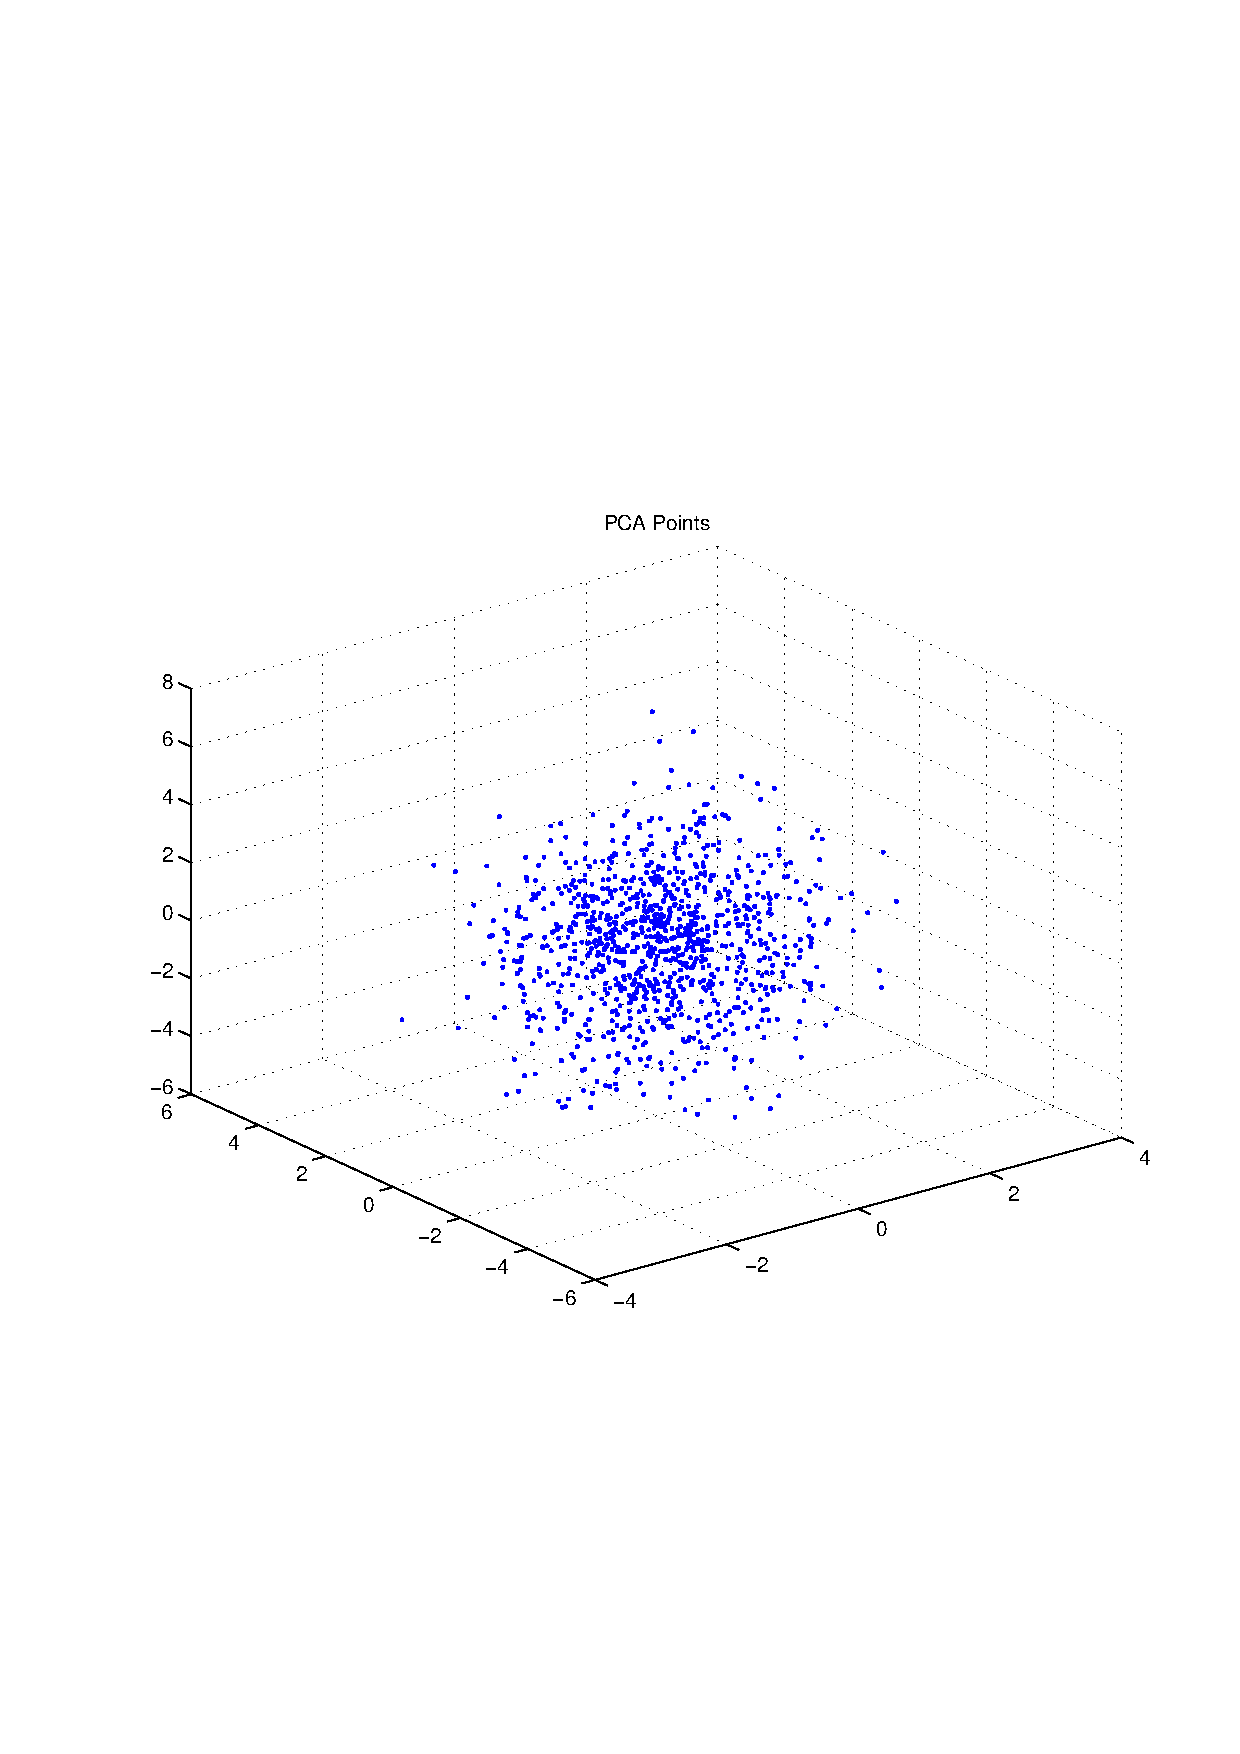
\includegraphics[width=10.0cm,height=10.0cm]{PCAPoints.pdf}

The eigenvectors:
+0.116, +0.221, +0.968
+0.173, +0.955, -0.239
-0.978, +0.195, +0.073

All of the eigenvalues of the covariance matrix:
(+0.958,+0.000), (+2.025,+0.000), (+3.017,+0.000)

QueryPerformanceCounter  =  +1.038
\subsubsection{Multi Variate Random Number Generator }
Sample from $N(\mu,\Sigma)$
mean= -0.002, variance=+1.004, skewness=+0.006, kurtosis=+3.003
mean= -0.001, variance=+1.017, skewness=-0.005, kurtosis=+2.988
mean= -0.002, variance=+1.006, skewness=-0.016, kurtosis=+3.014
Covariance Matrix 
+1.004, +0.009, +0.003
+0.009, +1.017, -0.003
+0.003, -0.003, +1.006

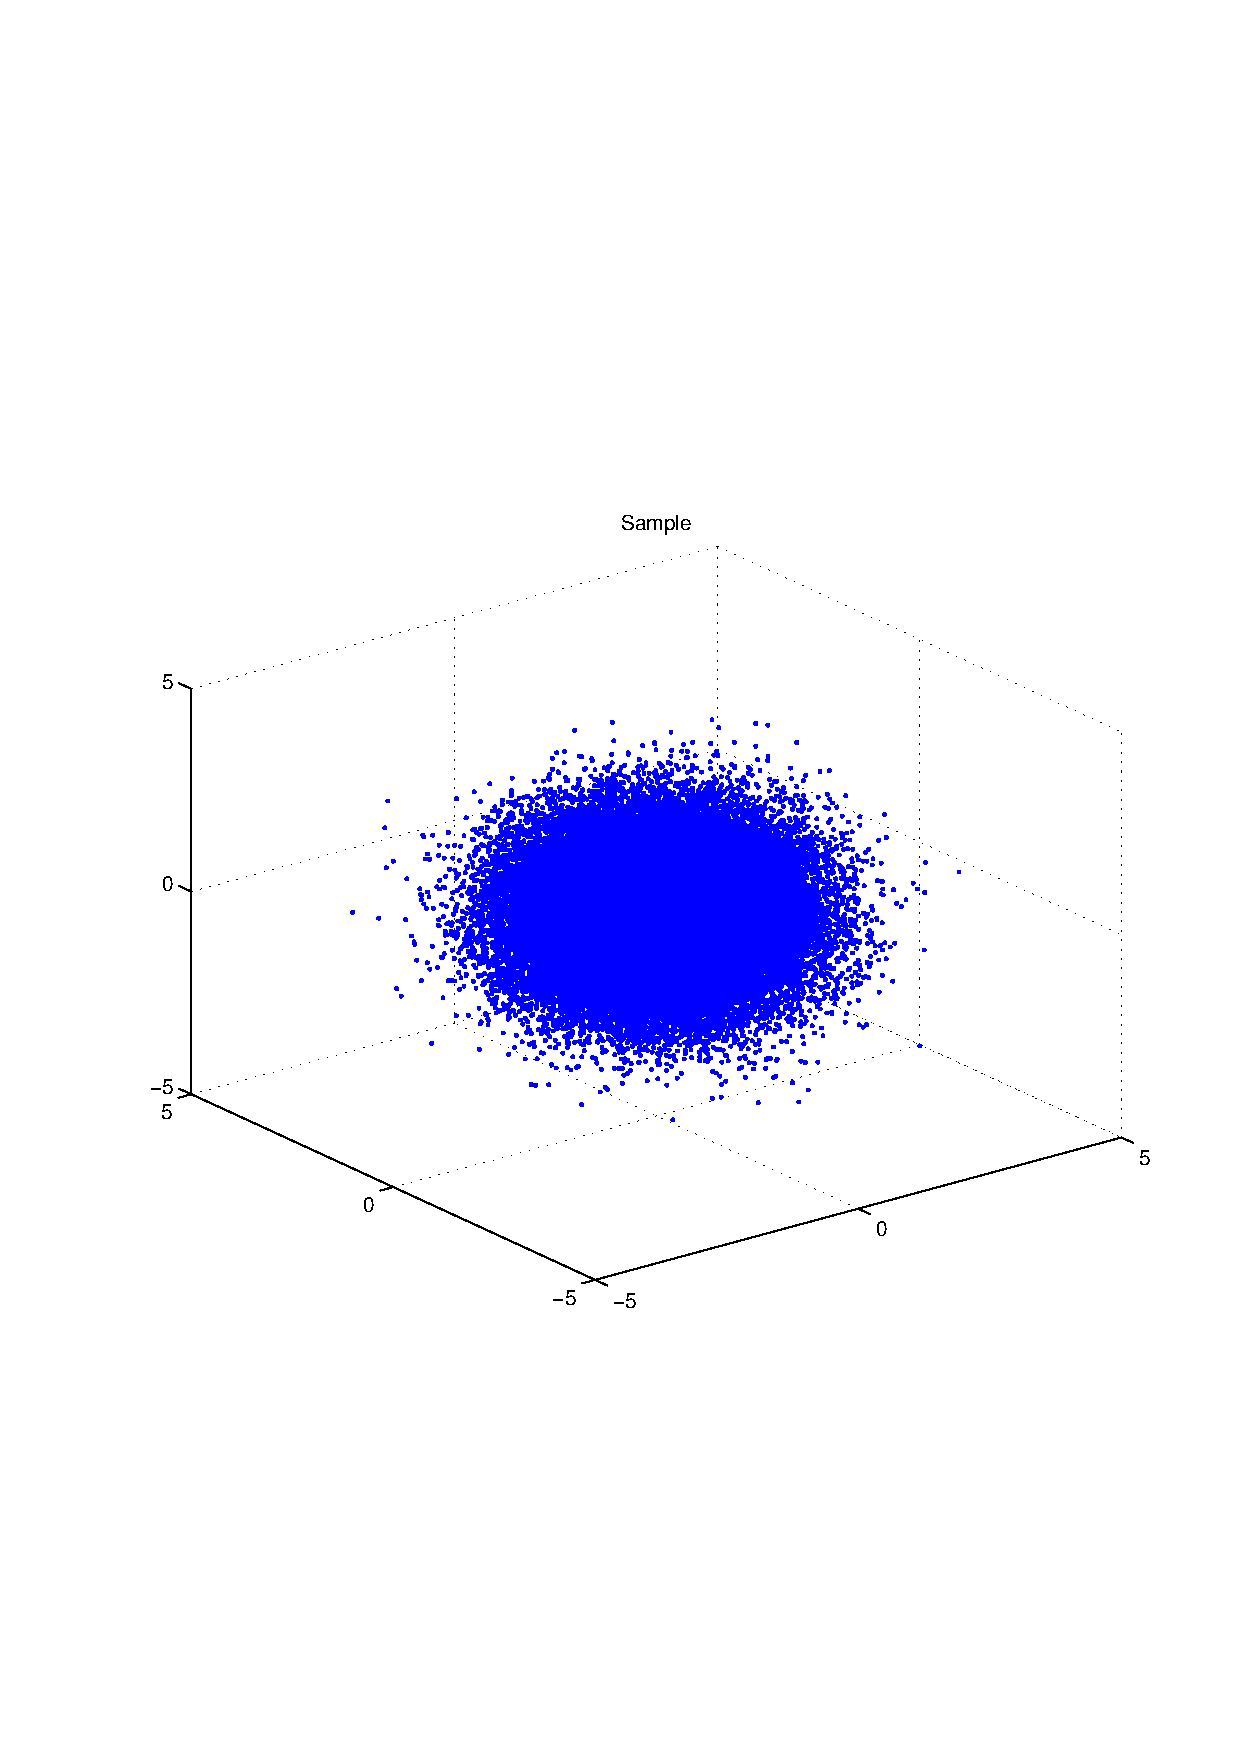
\includegraphics[width=10.0cm,height=10.0cm]{R_3_Normal.pdf}

Generate a sample from a unifom mixture of three Gaussians in $R^3$
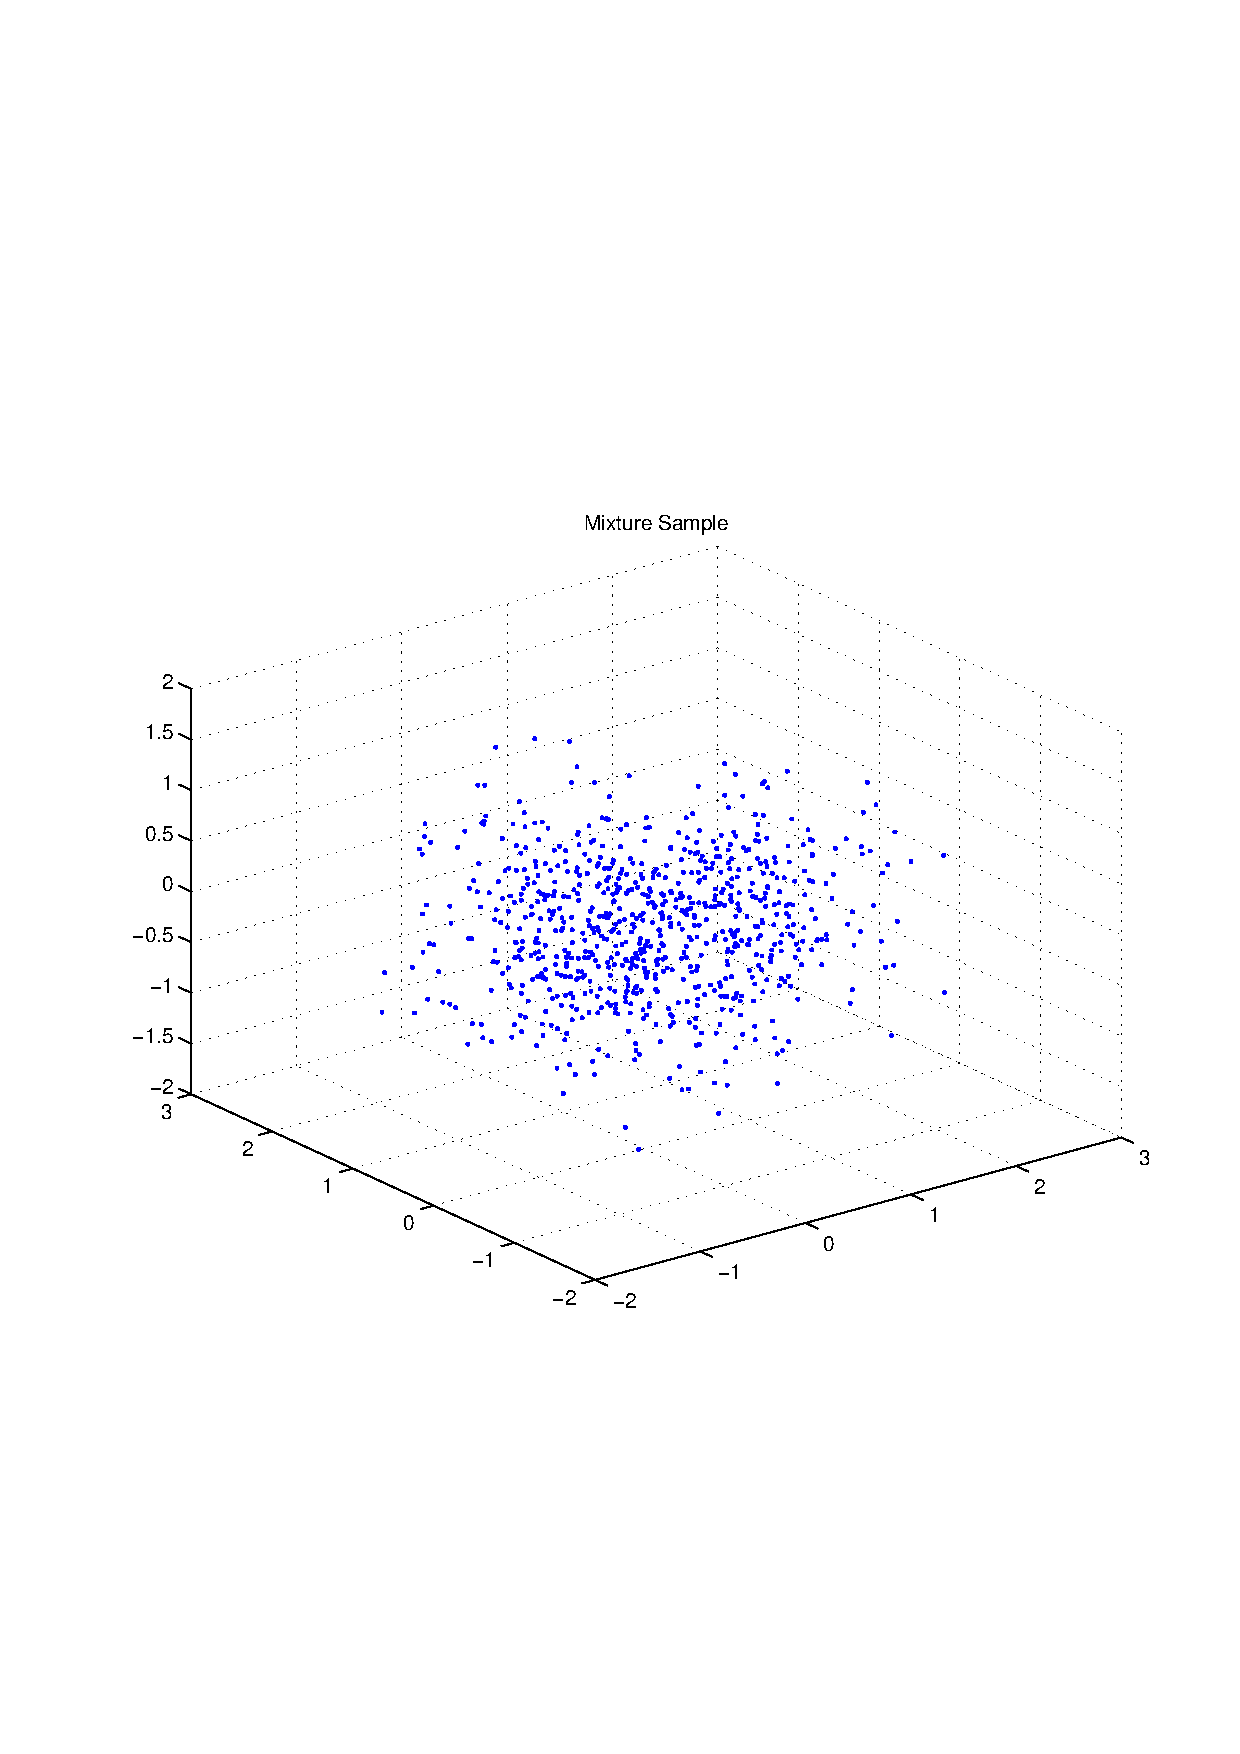
\includegraphics[width=10.0cm,height=10.0cm]{R_3_Normal_Mixture.pdf}

QueryPerformanceCounter  =  +16.725
\subsubsection{Matrix Multiply}
Comparing naive matrix multiply verus Intel MKL dgemm for matrix of size +2048.
This is for type double (hence the d in dgemm).
Naive type double matrix multiply tic toc  =  +0.401
dgemm plus row to column major transpose operation tic toc  =  +0.344
Comparing naive matrix multiply verus Intel MKL sgemm for matrix of size +2048.
This is for type float (hence the s in dgemm).
Naive type float matrix multiply tic toc  =  +0.331
sgemm plus row to column major transpose operation tic toc  =  +0.242
QueryPerformanceCounter  =  +1.474
\subsubsection{Descriptive Statistics}
Mean N(0,1): +0.003
Variance N(0,1): +1.006
Mean N(0,1) [recurrence relation method] :+0.003
Variance [recurrence relation method] :+1.006
Skewness : +0.007
Kurtosis : +2.997
QueryPerformanceCounter  =  +0.033
\subsubsection{Time Series }
+0.093
+0.726
+0.011
+2.178
QueryPerformanceCounter  =  +0.050
QueryPerformanceCounter  =  +6.928
\subsubsection{Iterated Exponential Filtering }
$\mu_1 =+0.093$
$\mu_2 =+0.726$
$\mu_3 =+0.011$
$\mu_4 =+2.178$
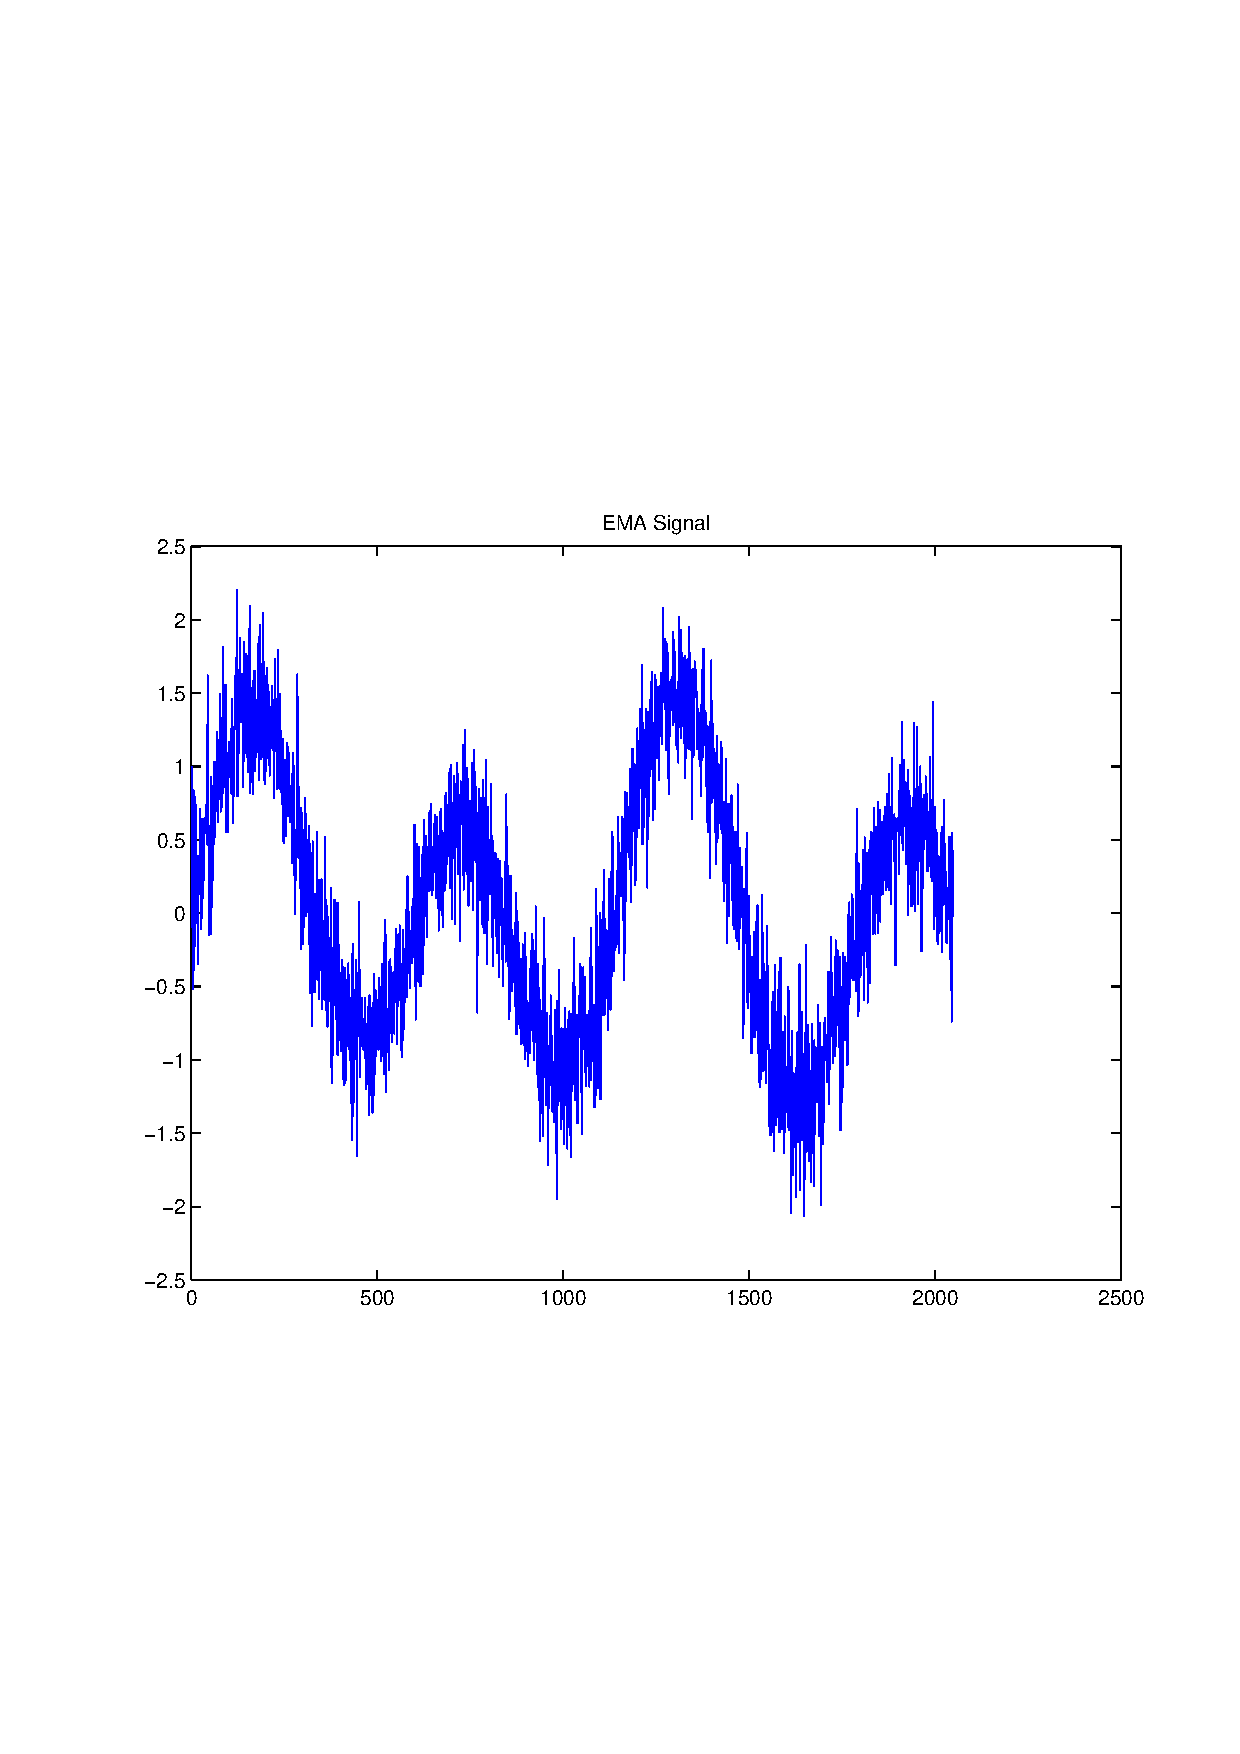
\includegraphics[width=10.0cm,height=10.0cm]{EMA_signal.pdf}

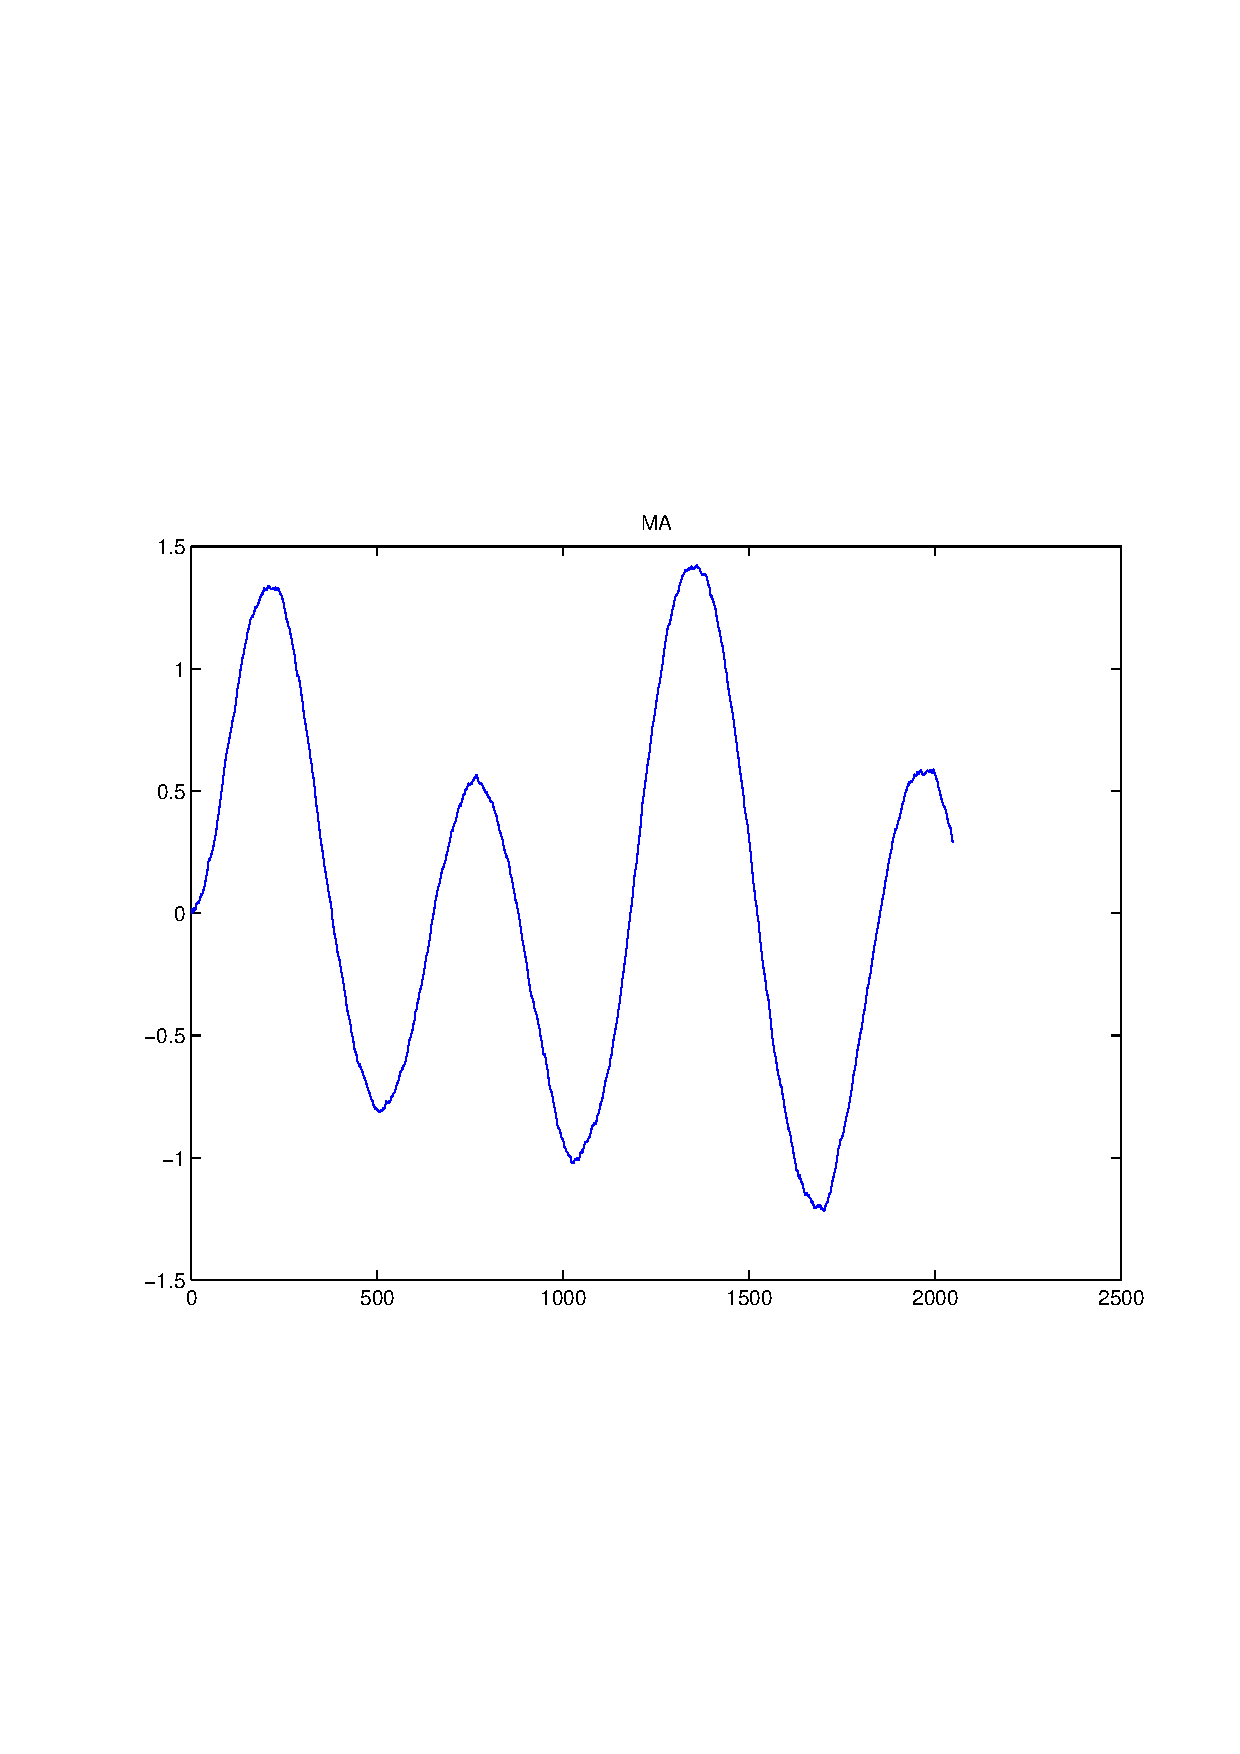
\includegraphics[width=10.0cm,height=10.0cm]{MA.pdf}

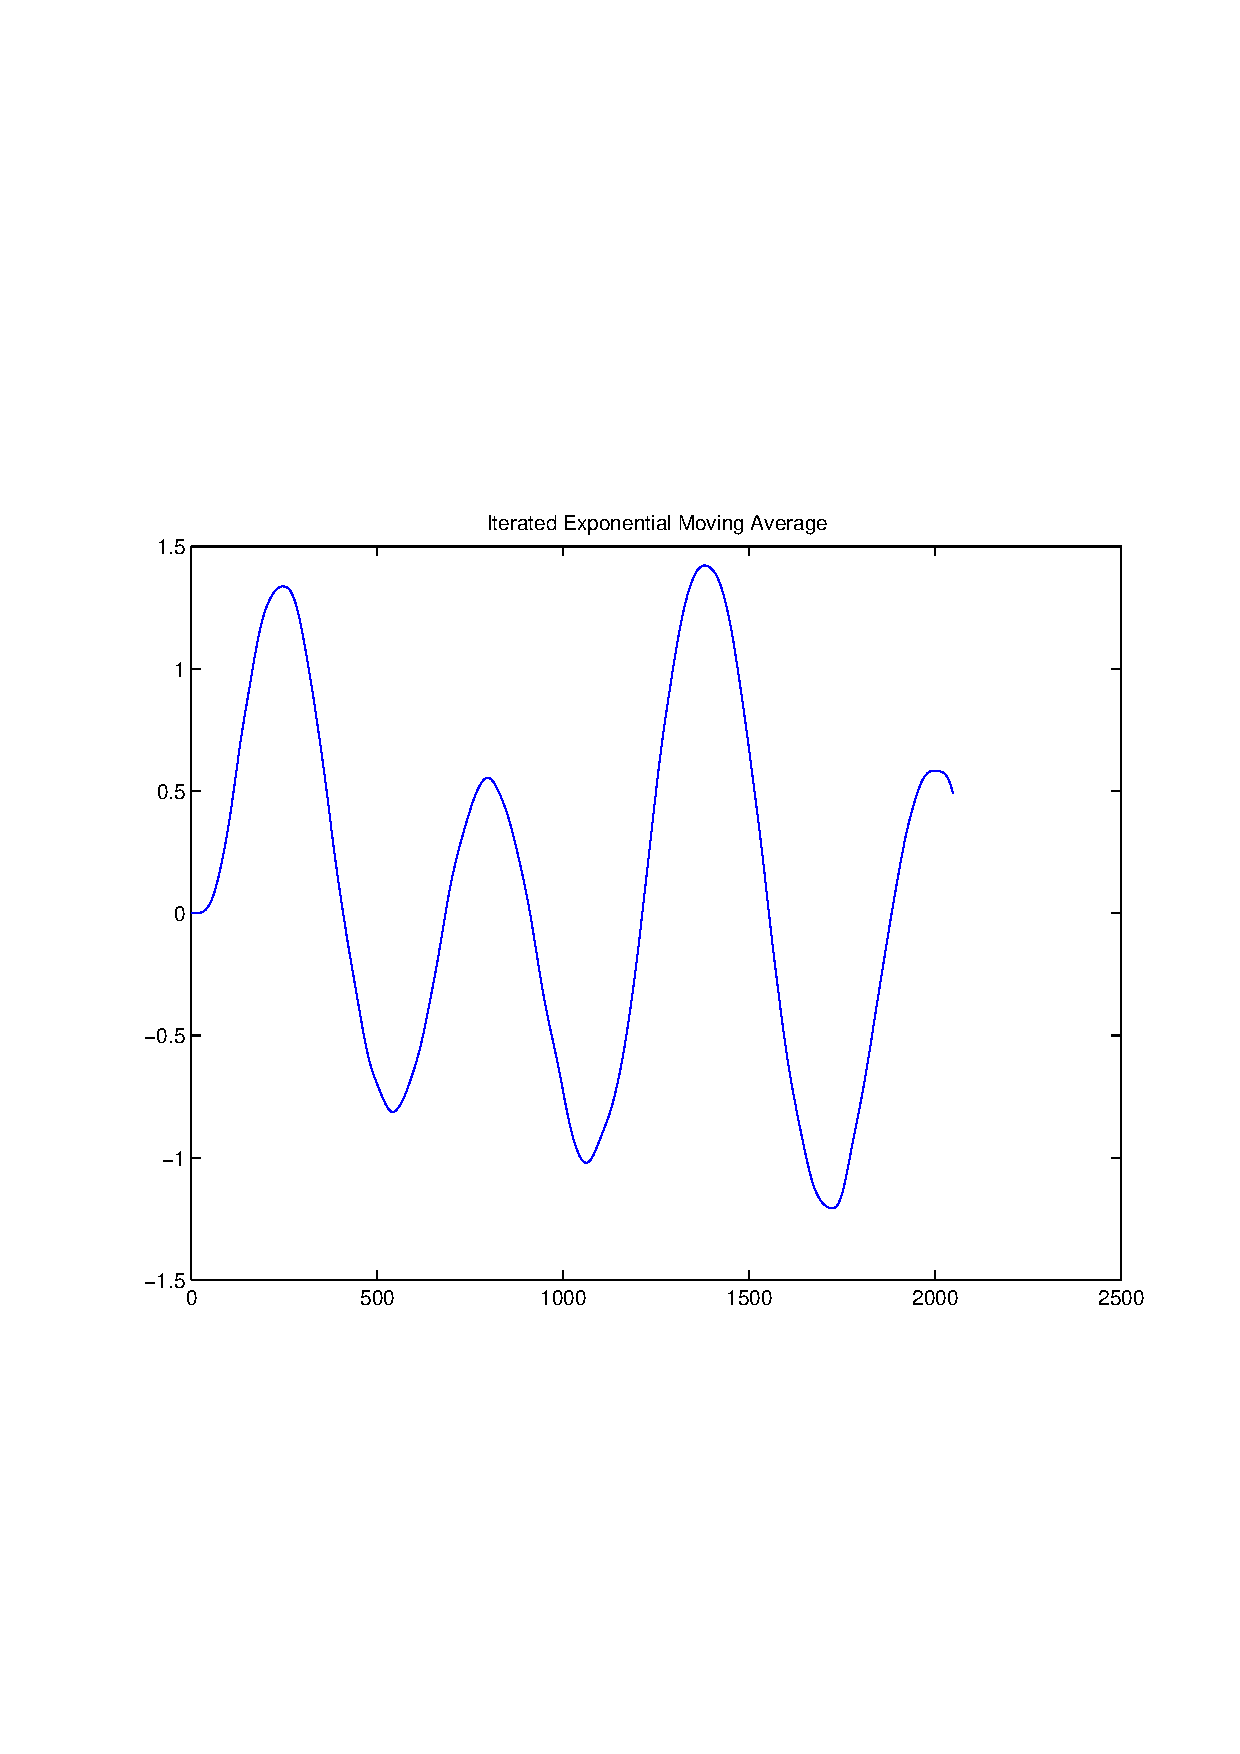
\includegraphics[width=10.0cm,height=10.0cm]{IEMA.pdf}

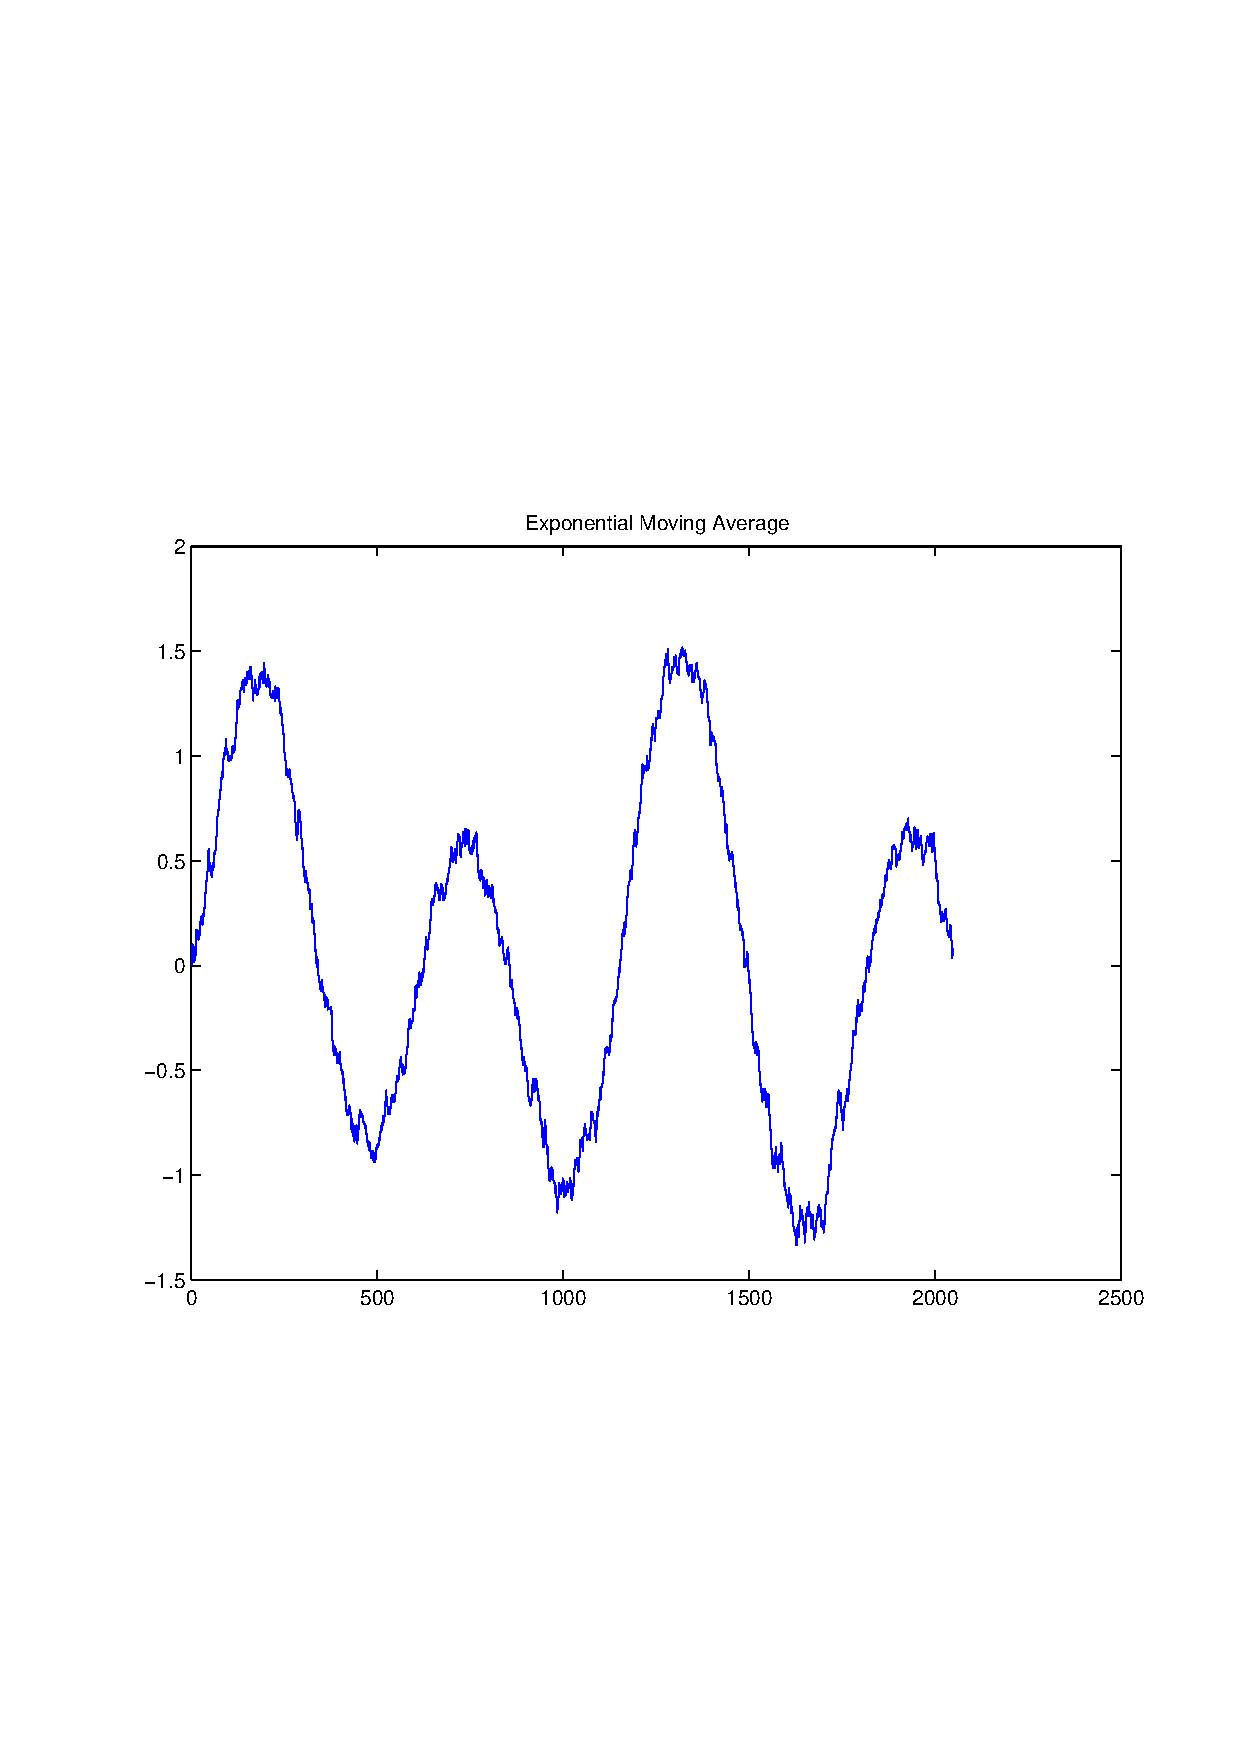
\includegraphics[width=10.0cm,height=10.0cm]{EMA.pdf}

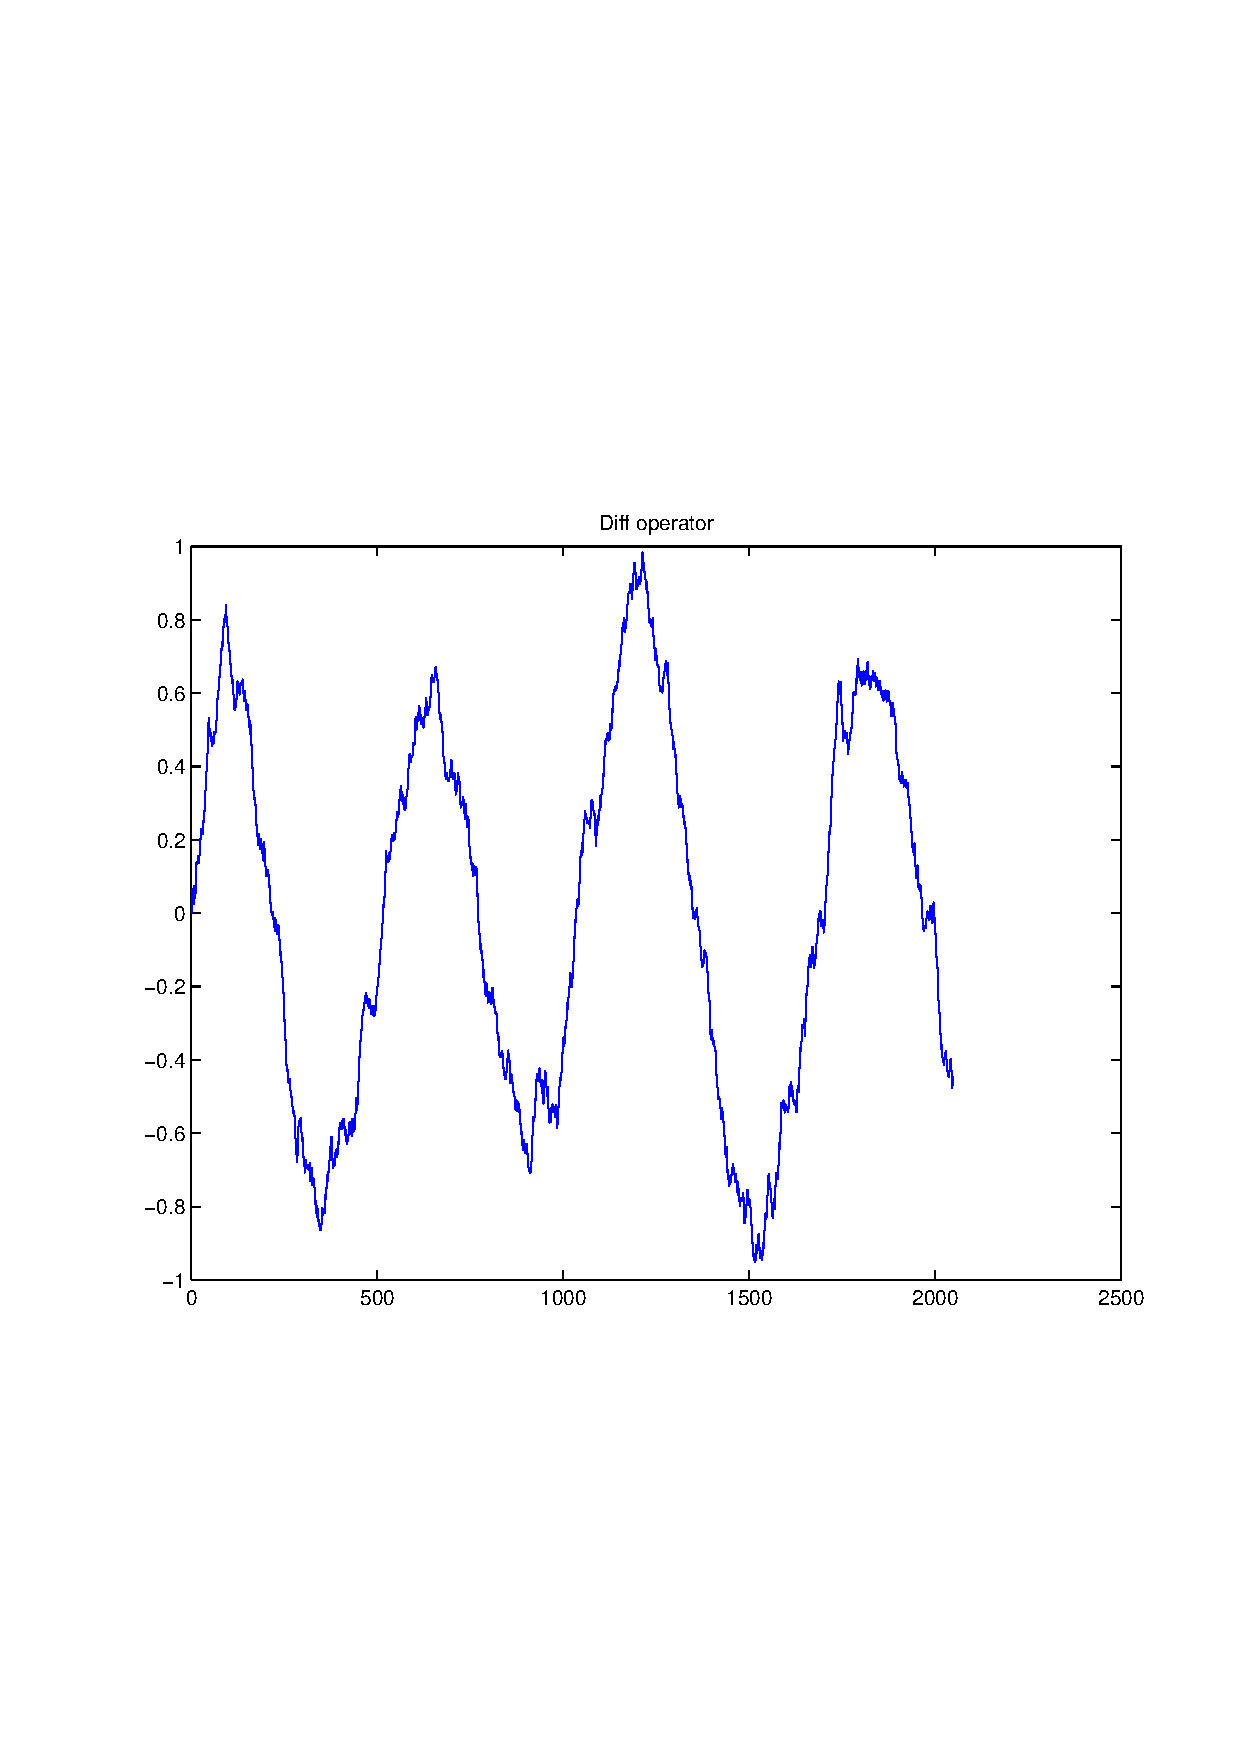
\includegraphics[width=10.0cm,height=10.0cm]{DIFF.pdf}

\includegraphics[width=10.0cm,height=10.0cm]{IteratedExponentailOperators.pdf}

\includegraphics[width=10.0cm,height=10.0cm]{IteratedExponentailOperators.pdf}

QueryPerformanceCounter  =  +8.267
\subsubsection{Testing binary writer}
Binary writer Speedup 1GB Double Matrix +54.590

Binary reader Speedup 1GB Double Matrix +306.044

Binary writer Speedup 1GB Double vector +9.694

Binary reader Speedup 1GB Double Matrix +190.054

QueryPerformanceCounter  =  +0.999
\subsubsection{Testing Gaussian Mixture Point Cloud and Latex Plotting Capabilities.}
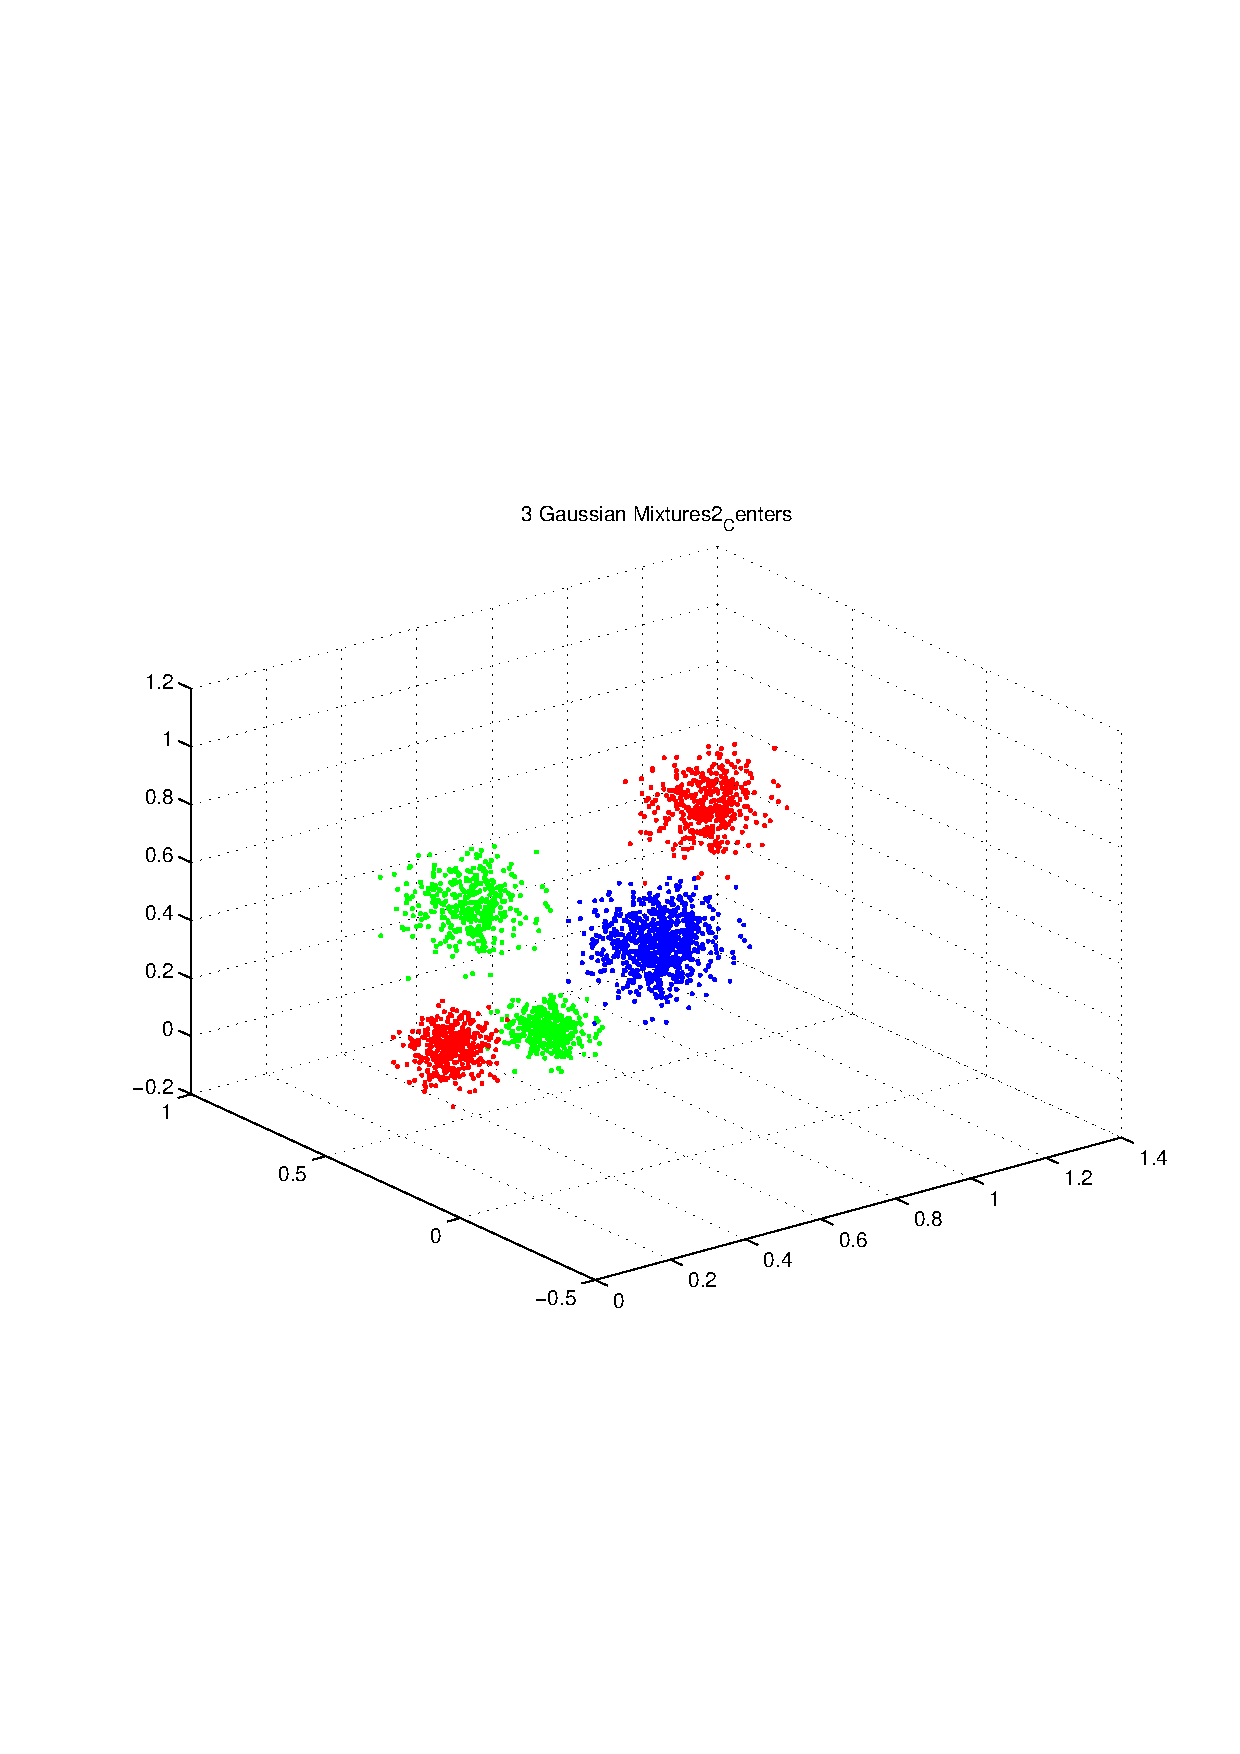
\includegraphics[width=10.0cm,height=10.0cm]{GaussianMixture_Dim_3_Centers2.pdf}

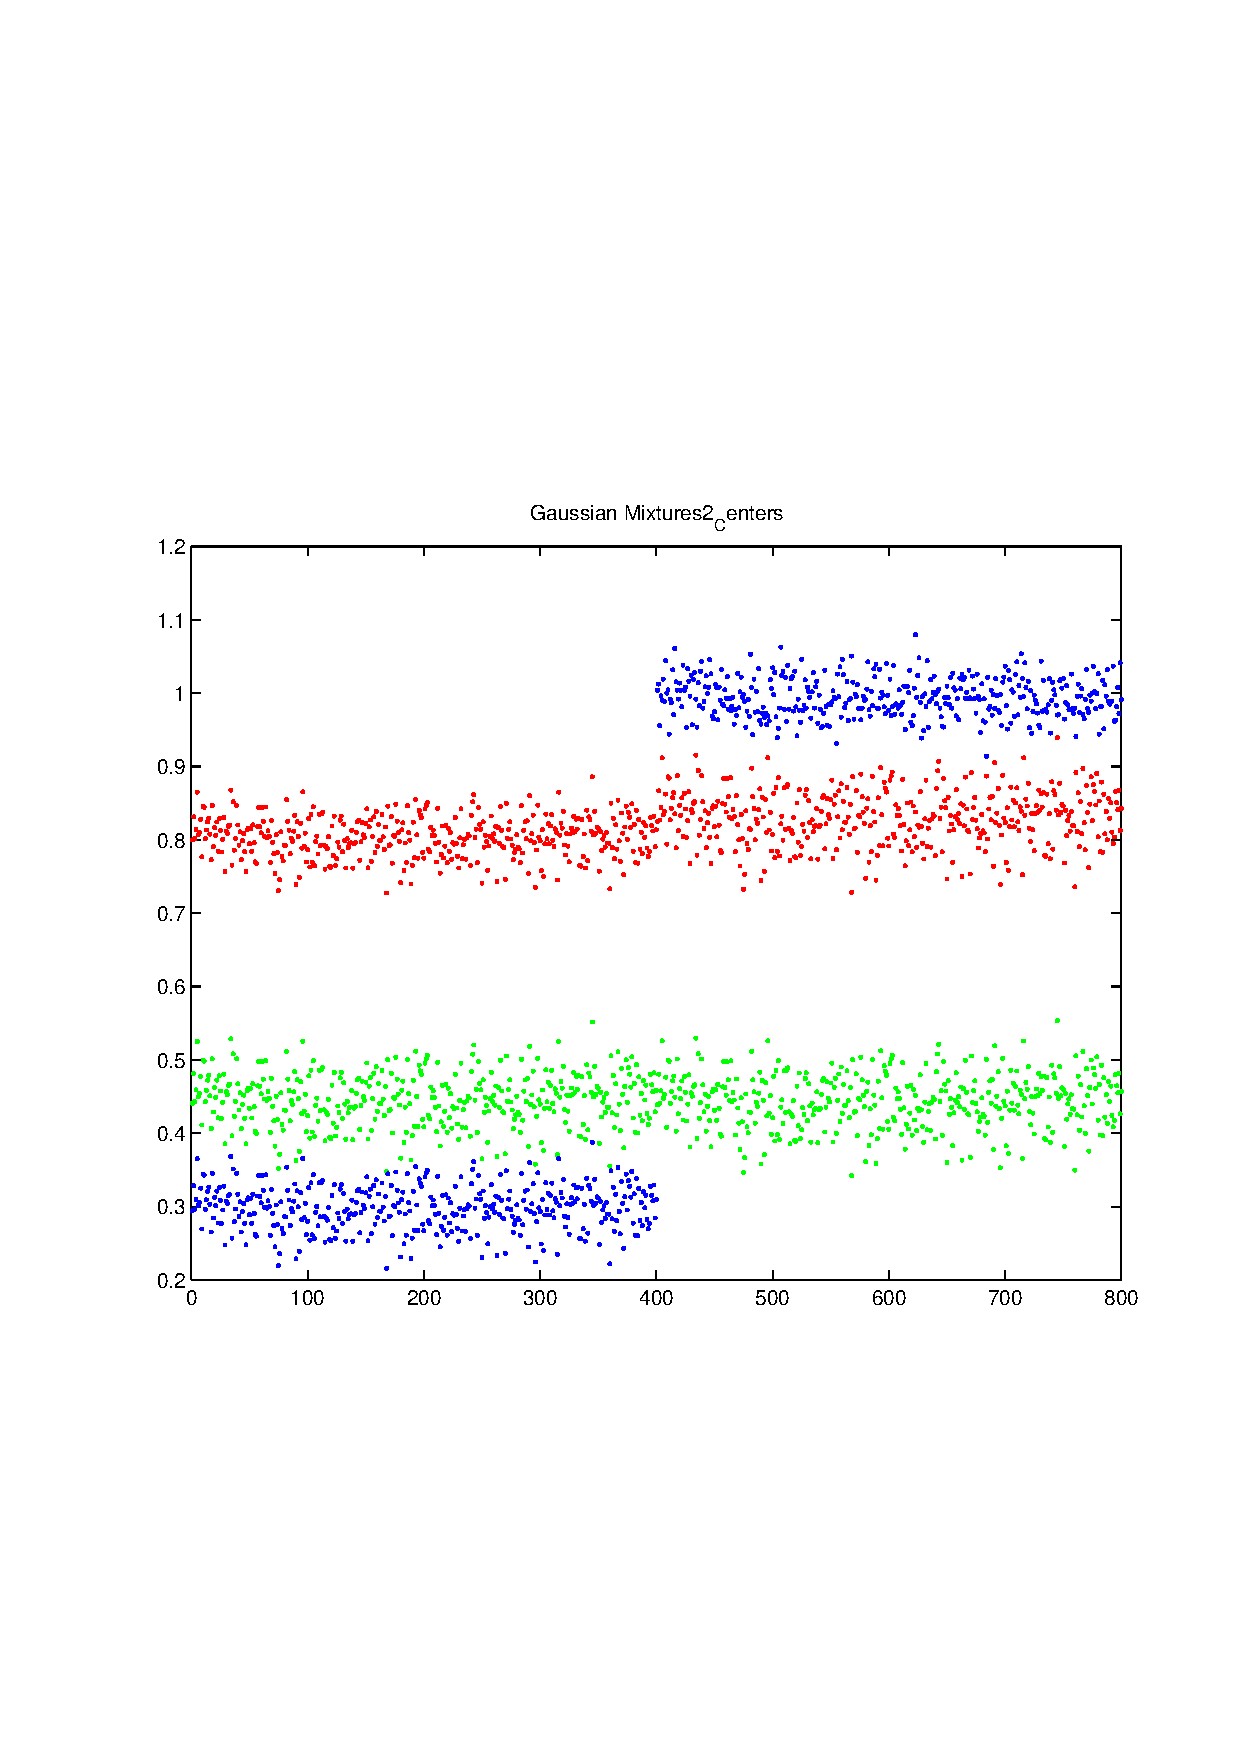
\includegraphics[width=10.0cm,height=10.0cm]{GaussianMixture_Dim_1_Centers2.pdf}

QueryPerformanceCounter  =  +2.947
\subsubsection{Intel VSL Function Check}
\includegraphics[width=10.0cm,height=10.0cm]{klVSLInv.pdf}

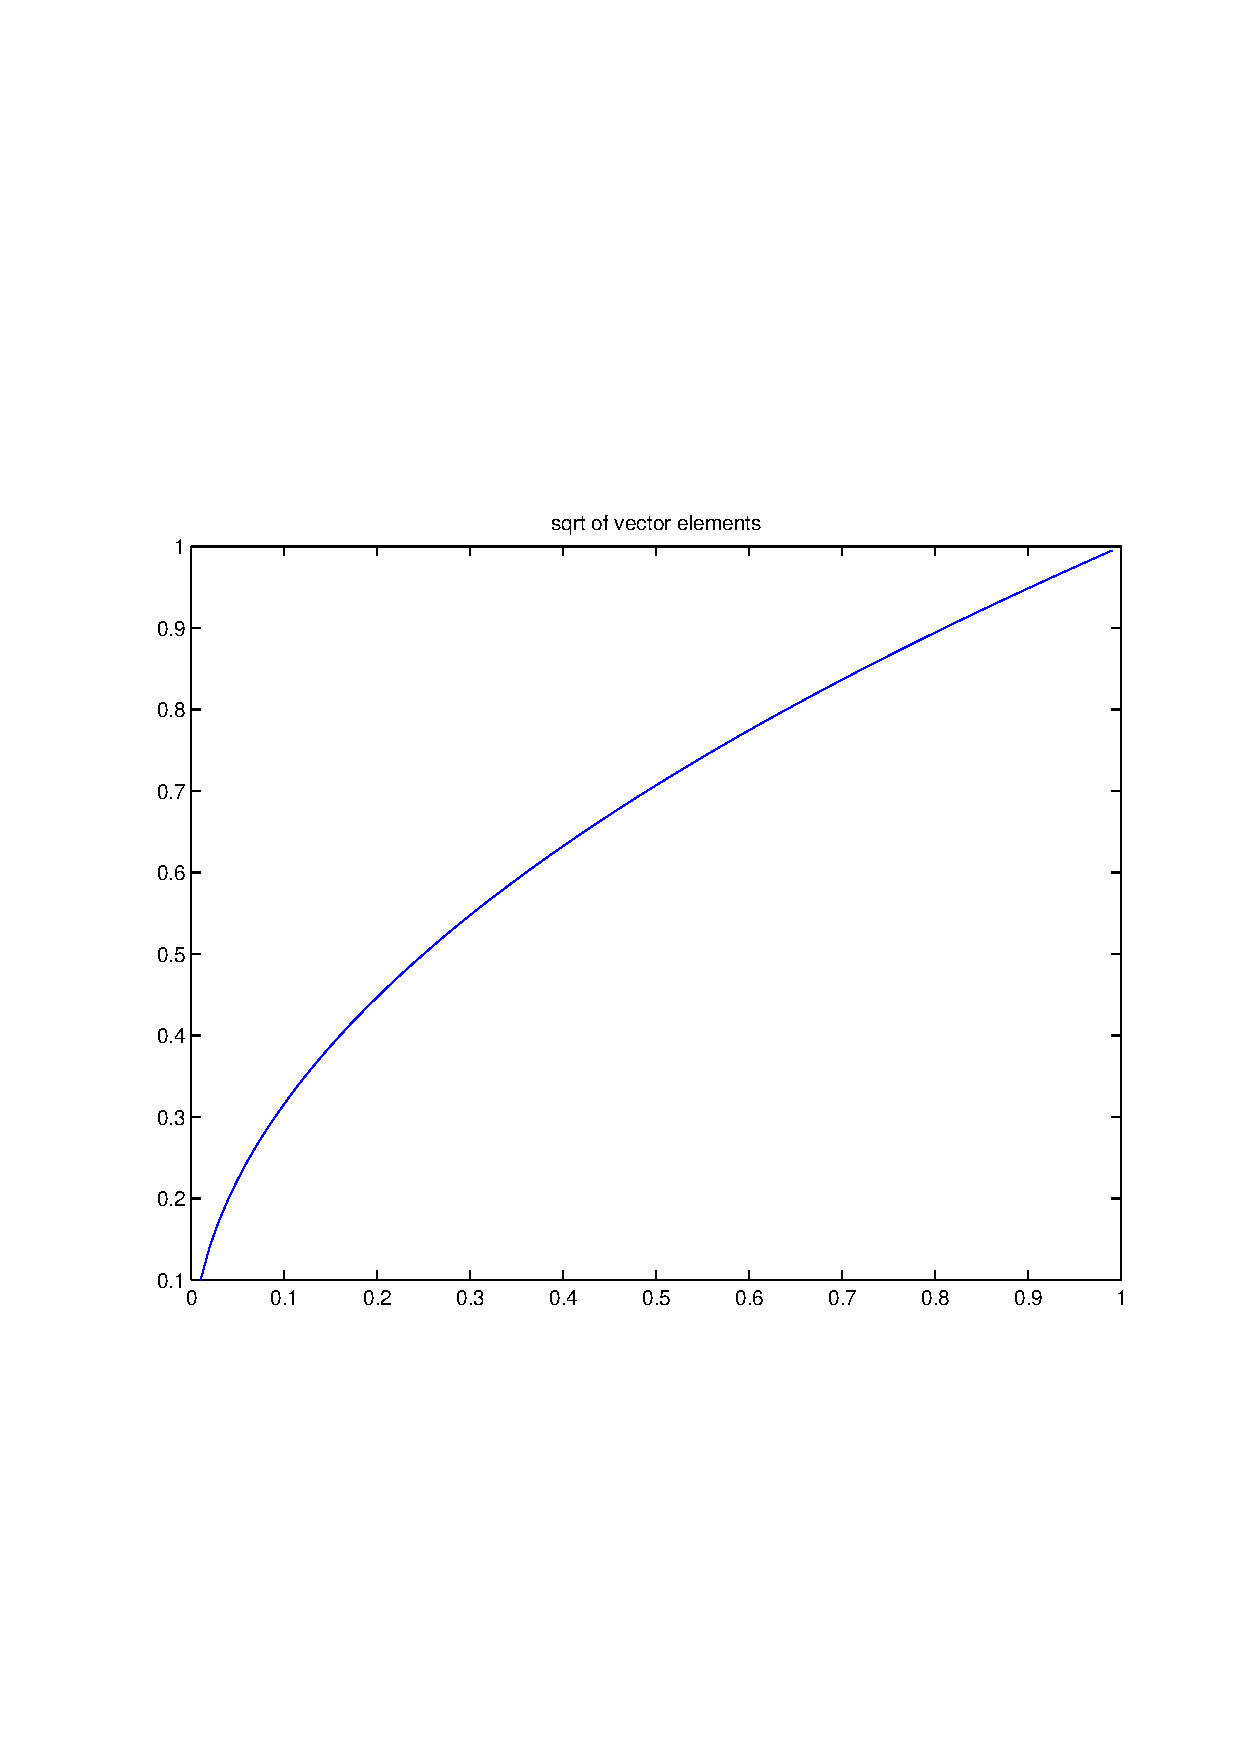
\includegraphics[width=10.0cm,height=10.0cm]{klVSLSqrt.pdf}

\includegraphics[width=10.0cm,height=10.0cm]{klVSLExp.pdf}

\includegraphics[width=10.0cm,height=10.0cm]{klVSLExpm1.pdf}

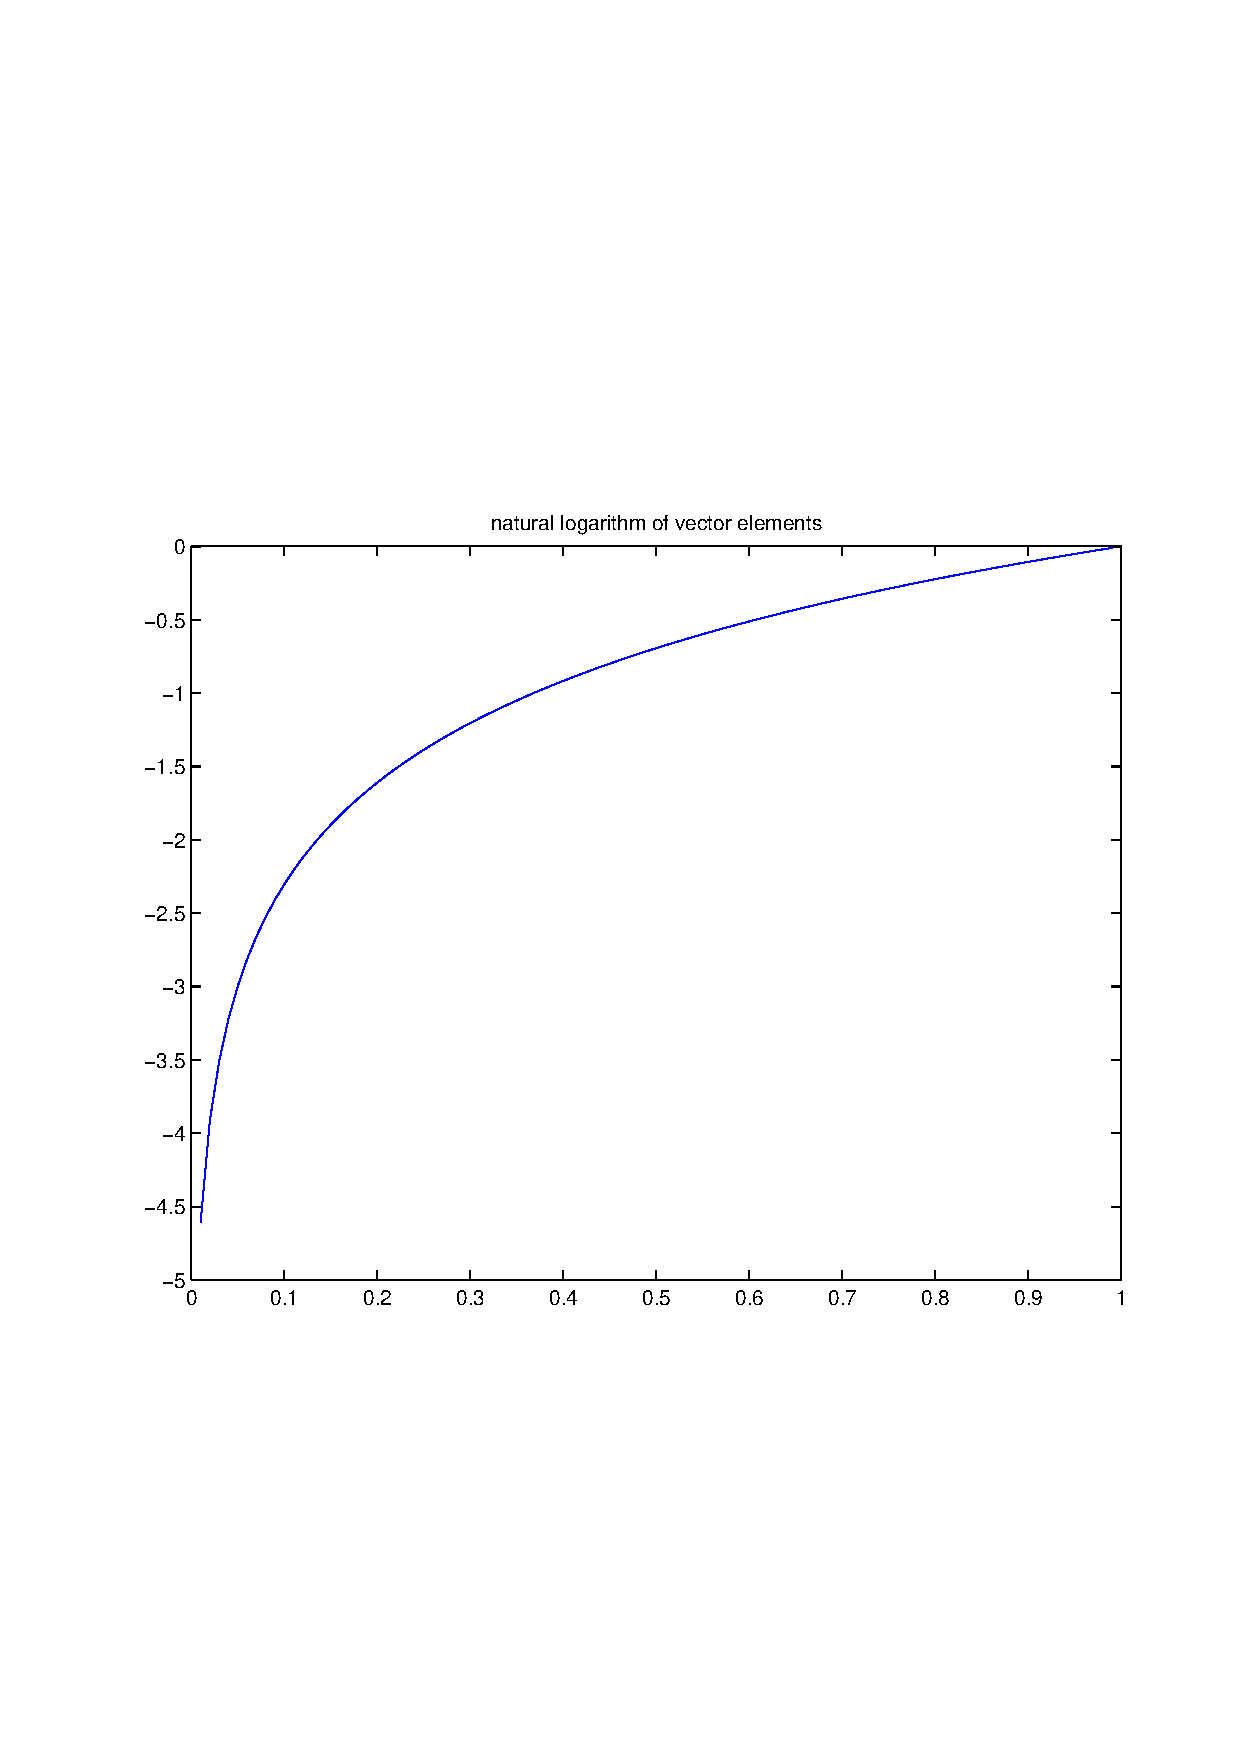
\includegraphics[width=10.0cm,height=10.0cm]{klVSLLn.pdf}

\includegraphics[width=10.0cm,height=10.0cm]{klVSLLog10.pdf}

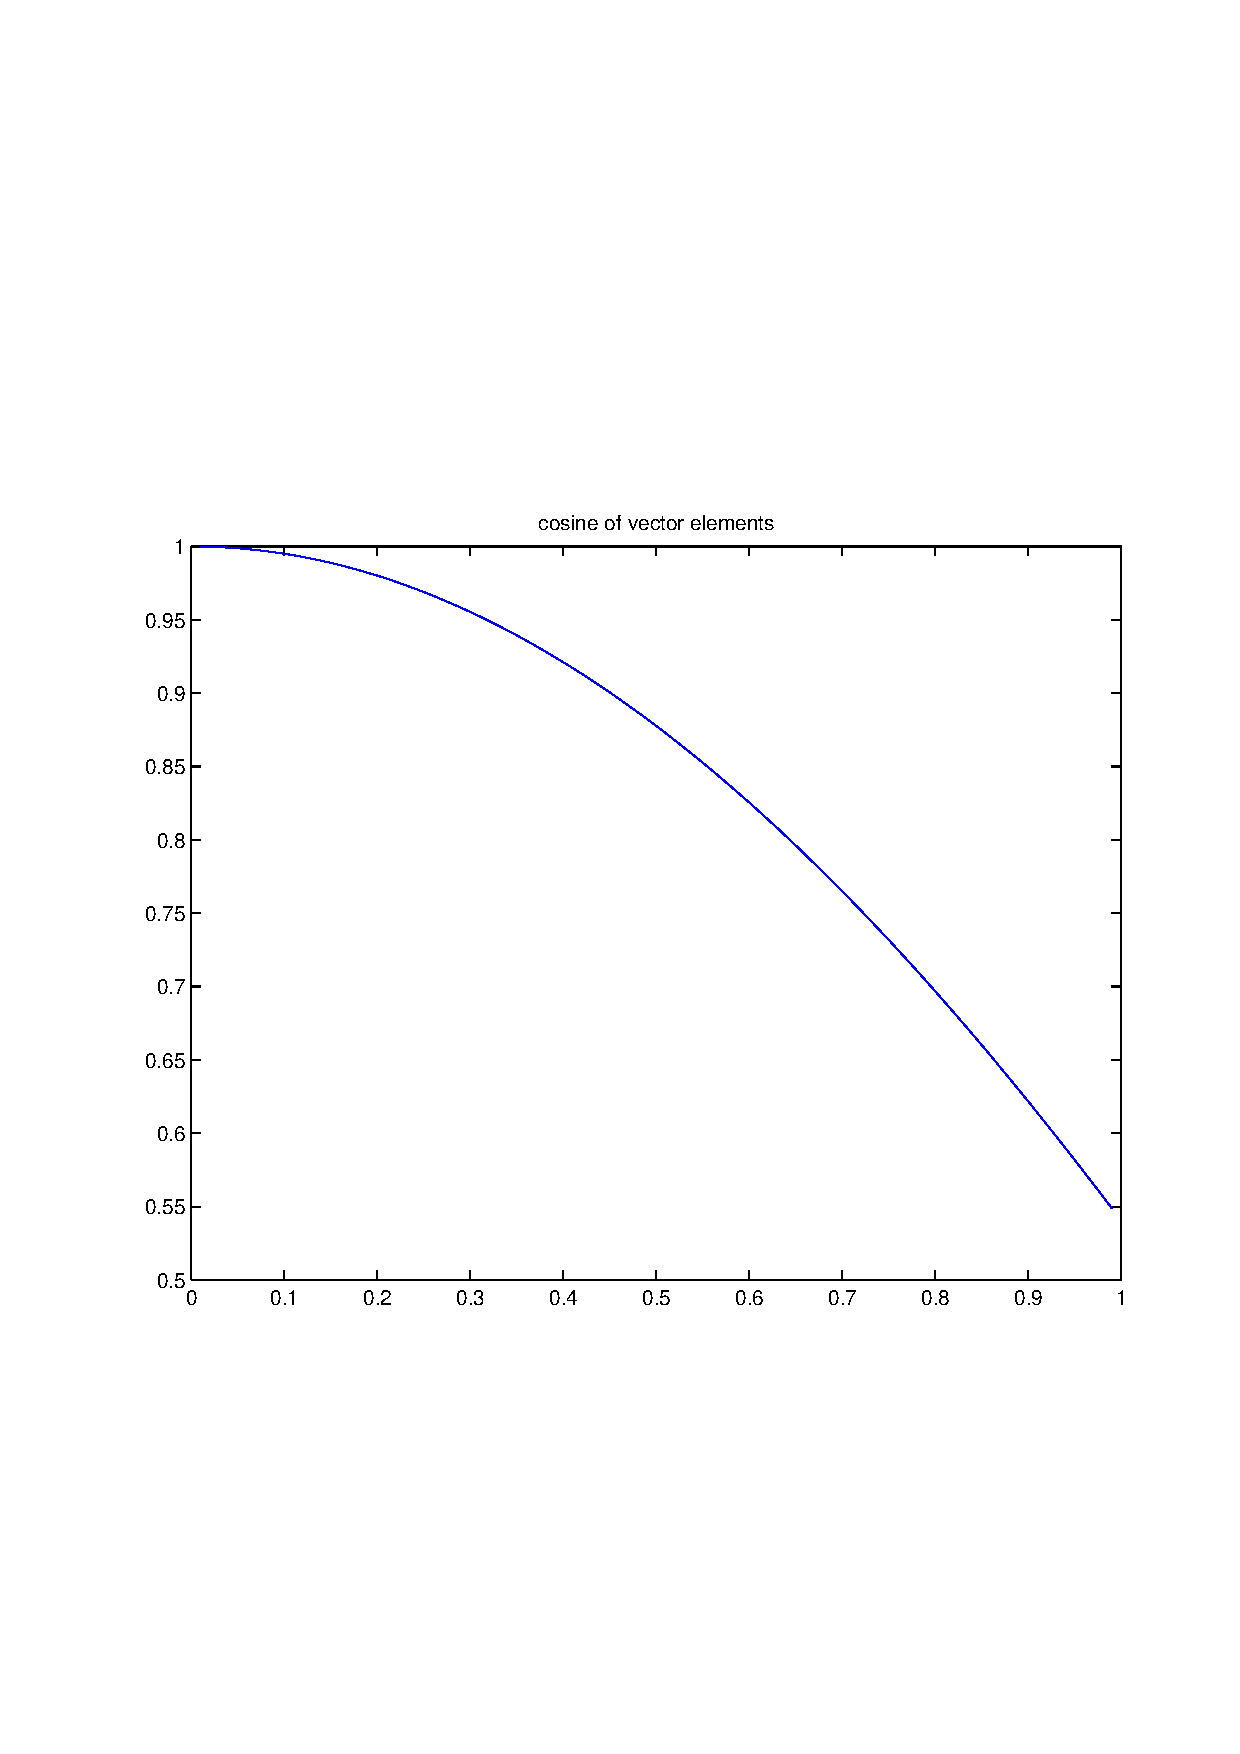
\includegraphics[width=10.0cm,height=10.0cm]{klVSLCos.pdf}

\includegraphics[width=10.0cm,height=10.0cm]{klVSLSin.pdf}

\includegraphics[width=10.0cm,height=10.0cm]{klVSLTan.pdf}

\includegraphics[width=10.0cm,height=10.0cm]{klVSLErf.pdf}

\includegraphics[width=10.0cm,height=10.0cm]{klVSLErfc.pdf}

\includegraphics[width=10.0cm,height=10.0cm]{klVSLCdfNorm.pdf}

\includegraphics[width=10.0cm,height=10.0cm]{klVSLErfInv.pdf}

\includegraphics[width=10.0cm,height=10.0cm]{klVSLLGamma.pdf}

\includegraphics[width=10.0cm,height=10.0cm]{klVSLTGamma.pdf}

QueryPerformanceCounter  =  +15.028
\subsubsection{Gram Matrix Consistency Check}
Sample Size = 4096
Feature dim = 3

$$Sigma$ = \left(
\begin{array}{
ccc}
+1.140 & +1.535 & +0.581 \\
+1.535 & +9.988 & +1.605 \\
+0.581 & +1.605 & +0.428 \\
\end{array}
\right)$ \newline 

$Sample Covariance = \left(
\begin{array}{
ccc}
+1.165 & +1.608 & +0.601 \\
+1.608 & +10.410 & +1.687 \\
+0.601 & +1.687 & +0.446 \\
\end{array}
\right)$ \newline 

$Sample Mean = \left(
\begin{array}{
ccc}
+1.00179 & +0.96875 & +0.99691 \\
\end{array}
\right)$ \newline 

$Sample Covariance-$Omega$ = \left(
\begin{array}{
ccc}
+0.025 & +0.073 & +0.019 \\
+0.073 & +0.421 & +0.082 \\
+0.019 & +0.082 & +0.018 \\
\end{array}
\right)$ \newline 

$Sample Covariance Eigs = \left(
\begin{array}{
ccc}
(+10.97685,+0.00000) & (+1.00338,+0.00000) & (+0.04000,+0.00000) \\
\end{array}
\right)$ \newline 

$Centered Mean = \left(
\begin{array}{
ccc}
-0.00000 & -0.00000 & +0.00000 \\
\end{array}
\right)$ \newline 

$Centered Covariance = \left(
\begin{array}{
ccc}
+1.165 & +1.608 & +0.601 \\
+1.608 & +10.410 & +1.687 \\
+0.601 & +1.687 & +0.446 \\
\end{array}
\right)$ \newline 

$Gram Matrix Gf Not scaled by sample size = \left(
\begin{array}{
ccc}
+4771.937 & +6584.578 & +2459.151 \\
+6584.578 & +42637.480 & +6908.824 \\
+2459.151 & +6908.824 & +1825.446 \\
\end{array}
\right)$ \newline 

$Gram Matrix Gf  scaled by sample size = \left(
\begin{array}{
ccc}
+1.165 & +1.608 & +0.600 \\
+1.608 & +10.410 & +1.687 \\
+0.600 & +1.687 & +0.446 \\
\end{array}
\right)$ \newline 

$SampleCovariance - Scaled Gf = \left(
\begin{array}{
ccc}
+0.000 & +0.000 & +0.000 \\
+0.000 & +0.003 & +0.000 \\
+0.000 & +0.000 & +0.000 \\
\end{array}
\right)$ \newline 

$EigenDecomp of SampleCovariance = \left(
\begin{array}{
ccc}
-0.169 & -0.972 & -0.165 \\
+0.918 & -0.217 & +0.333 \\
-0.359 & -0.095 & +0.928 \\
\end{array}
\right)$ \newline 

$EigenDecomp of Gram Matrix = \left(
\begin{array}{
ccc}
-0.118 & -0.975 & -0.189 \\
-0.319 & +0.218 & -0.922 \\
+0.940 & -0.049 & -0.337 \\
\end{array}
\right)$ \newline 

QueryPerformanceCounter  =  +1.376
\subsubsection{Eigen Solver Checks}
\subsubsection{Haar Distributed Random Orthogonal Matrix $A \in O(n)$}
 Testing Operator Norm
Number of Dimensions: +8

$A = \left(
\begin{array}{
cccccccc}
+0.022 & -0.024 & -0.741 & +0.417 & -0.364 & +0.291 & -0.243 & -0.026 \\
+0.195 & -0.655 & +0.212 & +0.215 & +0.316 & +0.099 & -0.562 & +0.127 \\
+0.336 & +0.153 & -0.221 & -0.537 & +0.160 & +0.013 & -0.392 & -0.589 \\
+0.869 & -0.081 & +0.005 & -0.003 & -0.296 & -0.198 & +0.246 & +0.226 \\
-0.099 & -0.215 & +0.439 & -0.174 & -0.724 & +0.357 & -0.085 & -0.251 \\
-0.193 & -0.595 & -0.403 & -0.562 & -0.006 & +0.007 & +0.302 & +0.197 \\
-0.157 & +0.220 & -0.021 & -0.285 & -0.308 & -0.420 & -0.558 & +0.513 \\
+0.151 & +0.303 & +0.048 & -0.253 & +0.190 & +0.750 & -0.034 & +0.469 \\
\end{array}
\right)$ \newline 

$Det(A) :   A \in O(n)$ = (+1.000,+0.000)

$L = \left(
\begin{array}{
cccccccc}
+1.000 & +0.000 & +0.000 & +0.000 & +0.000 & +0.000 & +0.000 & +0.000 \\
+0.225 & +1.000 & +0.000 & +0.000 & +0.000 & +0.000 & +0.000 & +0.000 \\
+0.025 & +0.035 & +1.000 & +0.000 & +0.000 & +0.000 & +0.000 & +0.000 \\
-0.222 & +0.963 & +0.809 & +1.000 & +0.000 & +0.000 & +0.000 & +0.000 \\
-0.114 & +0.353 & -0.488 & +0.046 & +1.000 & +0.000 & +0.000 & +0.000 \\
+0.174 & -0.497 & -0.203 & +0.057 & -0.342 & +1.000 & +0.000 & +0.000 \\
-0.180 & -0.322 & -0.064 & +0.172 & +0.223 & -0.385 & +1.000 & +0.000 \\
+0.387 & -0.289 & +0.217 & +0.510 & -0.504 & +0.460 & +0.870 & +1.000 \\
\end{array}
\right)$ \newline 

$U = \left(
\begin{array}{
cccccccc}
+0.869 & -0.081 & +0.005 & -0.003 & -0.296 & -0.198 & +0.246 & +0.226 \\
+0.000 & -0.637 & +0.211 & +0.216 & +0.382 & +0.143 & -0.617 & +0.077 \\
+0.000 & +0.000 & -0.748 & +0.409 & -0.370 & +0.291 & -0.228 & -0.035 \\
+0.000 & +0.000 & +0.000 & -1.102 & -0.141 & -0.411 & +1.135 & +0.202 \\
+0.000 & +0.000 & +0.000 & +0.000 & -1.066 & +0.445 & -0.002 & -0.278 \\
+0.000 & +0.000 & +0.000 & +0.000 & +0.000 & +1.090 & -0.496 & +0.354 \\
+0.000 & +0.000 & +0.000 & +0.000 & +0.000 & +0.000 & -1.113 & +0.740 \\
+0.000 & +0.000 & +0.000 & +0.000 & +0.000 & +0.000 & +0.000 & -1.697 \\
\end{array}
\right)$ \newline 

$L * U  = \left(
\begin{array}{
cccccccc}
+0.869 & -0.081 & +0.005 & -0.003 & -0.296 & -0.198 & +0.246 & +0.226 \\
+0.195 & -0.655 & +0.212 & +0.215 & +0.316 & +0.099 & -0.562 & +0.127 \\
+0.022 & -0.024 & -0.741 & +0.417 & -0.364 & +0.291 & -0.243 & -0.026 \\
-0.193 & -0.595 & -0.403 & -0.562 & -0.006 & +0.007 & +0.302 & +0.197 \\
-0.099 & -0.215 & +0.439 & -0.174 & -0.724 & +0.357 & -0.085 & -0.251 \\
+0.151 & +0.303 & +0.048 & -0.253 & +0.190 & +0.750 & -0.034 & +0.469 \\
-0.157 & +0.220 & -0.021 & -0.285 & -0.308 & -0.420 & -0.558 & +0.513 \\
+0.336 & +0.153 & -0.221 & -0.537 & +0.160 & +0.013 & -0.392 & -0.589 \\
\end{array}
\right)$ \newline 

$Det(L) :    = (+1.000,+0.000)     Det(U) :    = (+1.000,+0.000)     Det(LU) :    = (+1.000,-0.000)$

$||A||_{L_1}$  = +2.446

$||A||_{L_{\infty}}$ = +2.481

$||A^{-1}||_{L_1}$  = +2.481

$||A^{-1}||_{L_{\infty}}$ = +2.446

$||A||_{L_{\infty}} * ||A^{-1}||_{L_{\infty}} = +6.069$

$||A||_{L_1} * ||A^{-1}||_{L_1} = +6.069$

Frobenious Norm  $||A||_{\textit{F}}$ via $\sum\limits_{i,j =0}^{n} \|A_{i,j}|$   of  $A \in O(n)$  +2.828

$L_1$ condition number of Haar Distributed Random Orthogonal Matrix $A \in O(n)$ +5.541

$A = \left(
\begin{array}{
cccccccc}
+0.022 & -0.024 & -0.741 & +0.417 & -0.364 & +0.291 & -0.243 & -0.026 \\
+0.195 & -0.655 & +0.212 & +0.215 & +0.316 & +0.099 & -0.562 & +0.127 \\
+0.336 & +0.153 & -0.221 & -0.537 & +0.160 & +0.013 & -0.392 & -0.589 \\
+0.869 & -0.081 & +0.005 & -0.003 & -0.296 & -0.198 & +0.246 & +0.226 \\
-0.099 & -0.215 & +0.439 & -0.174 & -0.724 & +0.357 & -0.085 & -0.251 \\
-0.193 & -0.595 & -0.403 & -0.562 & -0.006 & +0.007 & +0.302 & +0.197 \\
-0.157 & +0.220 & -0.021 & -0.285 & -0.308 & -0.420 & -0.558 & +0.513 \\
+0.151 & +0.303 & +0.048 & -0.253 & +0.190 & +0.750 & -0.034 & +0.469 \\
\end{array}
\right)$ \newline 

$L_{\infty}$ condition number of Haar Distributed Random Orthogonal Matrix $A \in O(n)$ +6.010

Eigenvalues of $A \in O(n)$

(-0.027,+1.000), (-0.027,-1.000), (-0.725,+0.688), (-0.725,-0.688), (-1.000,+0.004), (-1.000,-0.004), (+0.921,+0.390), (+0.921,-0.390)

 $|\lambda | : \lambda \in \sigma(A) , A \in O(n)$

+1.000, +1.000, +1.000, +1.000, +1.000, +1.000, +1.000, +1.000


Calculating $A^{\dag} A,$  we expect $A^{\dag} A \approx I$

$A^{\dag} A = \left(
\begin{array}{
cccccccc}
+1.000 & +0.000 & +0.000 & -0.000 & +0.000 & +0.000 & -0.000 & -0.000 \\
+0.000 & +1.000 & +0.000 & -0.000 & -0.000 & +0.000 & -0.000 & -0.000 \\
+0.000 & +0.000 & +1.000 & +0.000 & +0.000 & +0.000 & -0.000 & +0.000 \\
-0.000 & -0.000 & +0.000 & +1.000 & +0.000 & +0.000 & +0.000 & +0.000 \\
+0.000 & -0.000 & +0.000 & +0.000 & +1.000 & +0.000 & -0.000 & -0.000 \\
+0.000 & +0.000 & +0.000 & +0.000 & +0.000 & +1.000 & +0.000 & -0.000 \\
-0.000 & -0.000 & -0.000 & +0.000 & -0.000 & +0.000 & +1.000 & +0.000 \\
-0.000 & -0.000 & +0.000 & +0.000 & -0.000 & -0.000 & +0.000 & +1.000 \\
\end{array}
\right)$ \newline 

Calculating $A^{-1} ,  A \in O(n)$.

$A^{-1} = \left(
\begin{array}{
cccccccc}
+0.022 & +0.195 & +0.336 & +0.869 & -0.099 & -0.193 & -0.157 & +0.151 \\
-0.024 & -0.655 & +0.153 & -0.081 & -0.215 & -0.595 & +0.220 & +0.303 \\
-0.741 & +0.212 & -0.221 & +0.005 & +0.439 & -0.403 & -0.021 & +0.048 \\
+0.417 & +0.215 & -0.537 & -0.003 & -0.174 & -0.562 & -0.285 & -0.253 \\
-0.364 & +0.316 & +0.160 & -0.296 & -0.724 & -0.006 & -0.308 & +0.190 \\
+0.291 & +0.099 & +0.013 & -0.198 & +0.357 & +0.007 & -0.420 & +0.750 \\
-0.243 & -0.562 & -0.392 & +0.246 & -0.085 & +0.302 & -0.558 & -0.034 \\
-0.026 & +0.127 & -0.589 & +0.226 & -0.251 & +0.197 & +0.513 & +0.469 \\
\end{array}
\right)$ \newline 

Calculating $A^{-1} *A  ,  A \in O(n)$.   We expect $A^{-1} *A  \approx I$. 

$A^{-1} *A = \left(
\begin{array}{
cccccccc}
+1.000 & -0.000 & -0.000 & -0.000 & -0.000 & +0.000 & -0.000 & -0.000 \\
+0.000 & +1.000 & +0.000 & -0.000 & -0.000 & -0.000 & +0.000 & +0.000 \\
+0.000 & +0.000 & +1.000 & -0.000 & +0.000 & -0.000 & +0.000 & +0.000 \\
-0.000 & -0.000 & -0.000 & +1.000 & -0.000 & -0.000 & +0.000 & -0.000 \\
-0.000 & +0.000 & -0.000 & +0.000 & +1.000 & +0.000 & -0.000 & -0.000 \\
+0.000 & -0.000 & +0.000 & -0.000 & +0.000 & +1.000 & +0.000 & +0.000 \\
+0.000 & -0.000 & -0.000 & +0.000 & -0.000 & -0.000 & +1.000 & -0.000 \\
+0.000 & +0.000 & +0.000 & +0.000 & -0.000 & +0.000 & +0.000 & +1.000 \\
\end{array}
\right)$ \newline 

Calculating SVD of  $A \in O(n)$

$U = \left(
\begin{array}{
cccccccc}
+0.111 & -0.505 & +0.428 & +0.361 & +0.208 & +0.471 & -0.353 & -0.169 \\
+0.853 & -0.112 & -0.186 & -0.205 & +0.102 & -0.221 & -0.078 & -0.343 \\
-0.465 & -0.428 & -0.286 & -0.141 & +0.287 & -0.462 & -0.318 & -0.320 \\
+0.117 & -0.287 & -0.047 & +0.637 & +0.178 & -0.407 & +0.494 & +0.233 \\
+0.117 & -0.549 & -0.011 & -0.347 & -0.334 & -0.062 & -0.140 & +0.656 \\
+0.104 & +0.369 & +0.236 & +0.316 & -0.080 & -0.454 & -0.654 & +0.238 \\
-0.075 & -0.168 & +0.307 & +0.087 & -0.763 & -0.234 & +0.135 & -0.457 \\
-0.022 & +0.024 & +0.741 & -0.417 & +0.364 & -0.291 & +0.243 & +0.026 \\
\end{array}
\right)$ \newline 

$S = \left(
\begin{array}{
cccccccc}
+1.000 & +0.000 & +0.000 & +0.000 & +0.000 & +0.000 & +0.000 & +0.000 \\
+0.000 & +1.000 & +0.000 & +0.000 & +0.000 & +0.000 & +0.000 & +0.000 \\
+0.000 & +0.000 & +1.000 & +0.000 & +0.000 & +0.000 & +0.000 & +0.000 \\
+0.000 & +0.000 & +0.000 & +1.000 & +0.000 & +0.000 & +0.000 & +0.000 \\
+0.000 & +0.000 & +0.000 & +0.000 & +1.000 & +0.000 & +0.000 & +0.000 \\
+0.000 & +0.000 & +0.000 & +0.000 & +0.000 & +1.000 & +0.000 & +0.000 \\
+0.000 & +0.000 & +0.000 & +0.000 & +0.000 & +0.000 & +1.000 & +0.000 \\
+0.000 & +0.000 & +0.000 & +0.000 & +0.000 & +0.000 & +0.000 & +1.000 \\
\end{array}
\right)$ \newline 

$V = \left(
\begin{array}{
cccccccc}
-0.000 & -0.000 & -0.000 & +0.000 & -0.000 & +0.000 & +0.000 & -1.000 \\
+0.810 & +0.167 & +0.282 & +0.106 & +0.356 & +0.224 & -0.219 & -0.000 \\
-0.051 & +0.667 & +0.270 & -0.644 & -0.242 & -0.034 & -0.074 & -0.000 \\
-0.142 & +0.667 & -0.514 & +0.325 & +0.371 & +0.067 & +0.152 & +0.000 \\
+0.313 & -0.167 & -0.228 & -0.456 & +0.229 & -0.150 & +0.735 & +0.000 \\
-0.235 & -0.000 & +0.375 & +0.000 & +0.592 & -0.666 & -0.104 & -0.000 \\
-0.392 & -0.167 & +0.144 & -0.302 & +0.504 & +0.672 & -0.033 & +0.000 \\
+0.118 & -0.167 & -0.609 & -0.412 & +0.142 & -0.163 & -0.610 & +0.000 \\
\end{array}
\right)$ \newline 

$U S V = \left(
\begin{array}{
cccccccc}
-0.409 & +0.494 & -0.031 & -0.131 & -0.024 & -0.658 & +0.352 & -0.111 \\
+0.021 & -0.227 & +0.115 & +0.159 & -0.267 & +0.103 & +0.317 & -0.853 \\
-0.028 & -0.297 & -0.215 & +0.189 & -0.549 & +0.007 & +0.558 & +0.465 \\
-0.336 & +0.195 & -0.685 & -0.119 & +0.227 & +0.518 & +0.178 & -0.117 \\
-0.352 & -0.360 & -0.346 & -0.239 & -0.412 & -0.256 & -0.566 & -0.117 \\
+0.609 & +0.512 & -0.386 & +0.126 & -0.391 & -0.068 & -0.185 & -0.104 \\
-0.455 & +0.415 & +0.375 & +0.308 & -0.412 & +0.393 & -0.235 & +0.075 \\
+0.131 & +0.115 & +0.248 & -0.860 & -0.288 & +0.251 & +0.150 & +0.022 \\
\end{array}
\right)$ \newline 

Calculating first few eigenvectors of $A \in O(n)$ using LAPACK syevx

\subsubsection{Wishart Matrix $A \in W(n)$}
$L_1$ condition number of Wishart Matrix +1489.694
$L_infty$ condition number of Wishart Matrix +1489.694
\subsubsection{Gaussian Orthogonal Ensemble $A \in GOE(n)$}
$L_1$ condition number of GOE Matrix +66.900
$L_\infty$ condition number of GOE Matrix +66.900
\subsubsection{The Identity Matrix $I \in M(n)$}
$L_1$ condition number of $I$ = +1.000
$L_\infty$ condition number of $I$ = +1.000
QueryPerformanceCounter  =  +0.306
\subsubsection{Generate Tracey Widom Sample}
\subsubsection{Sample from $W_n m$ times and calculate empirical PDF of the first eig}
Here we generate histograms of $\lambda_1$ for GOE (Gaussian Orthogonal Ensemble), and W (Wishart) 		 distributed of random matrices
These should approximate the celebrated Tracy Widom distribution.
Dimension $n = +128$

Sample size $m = 32$

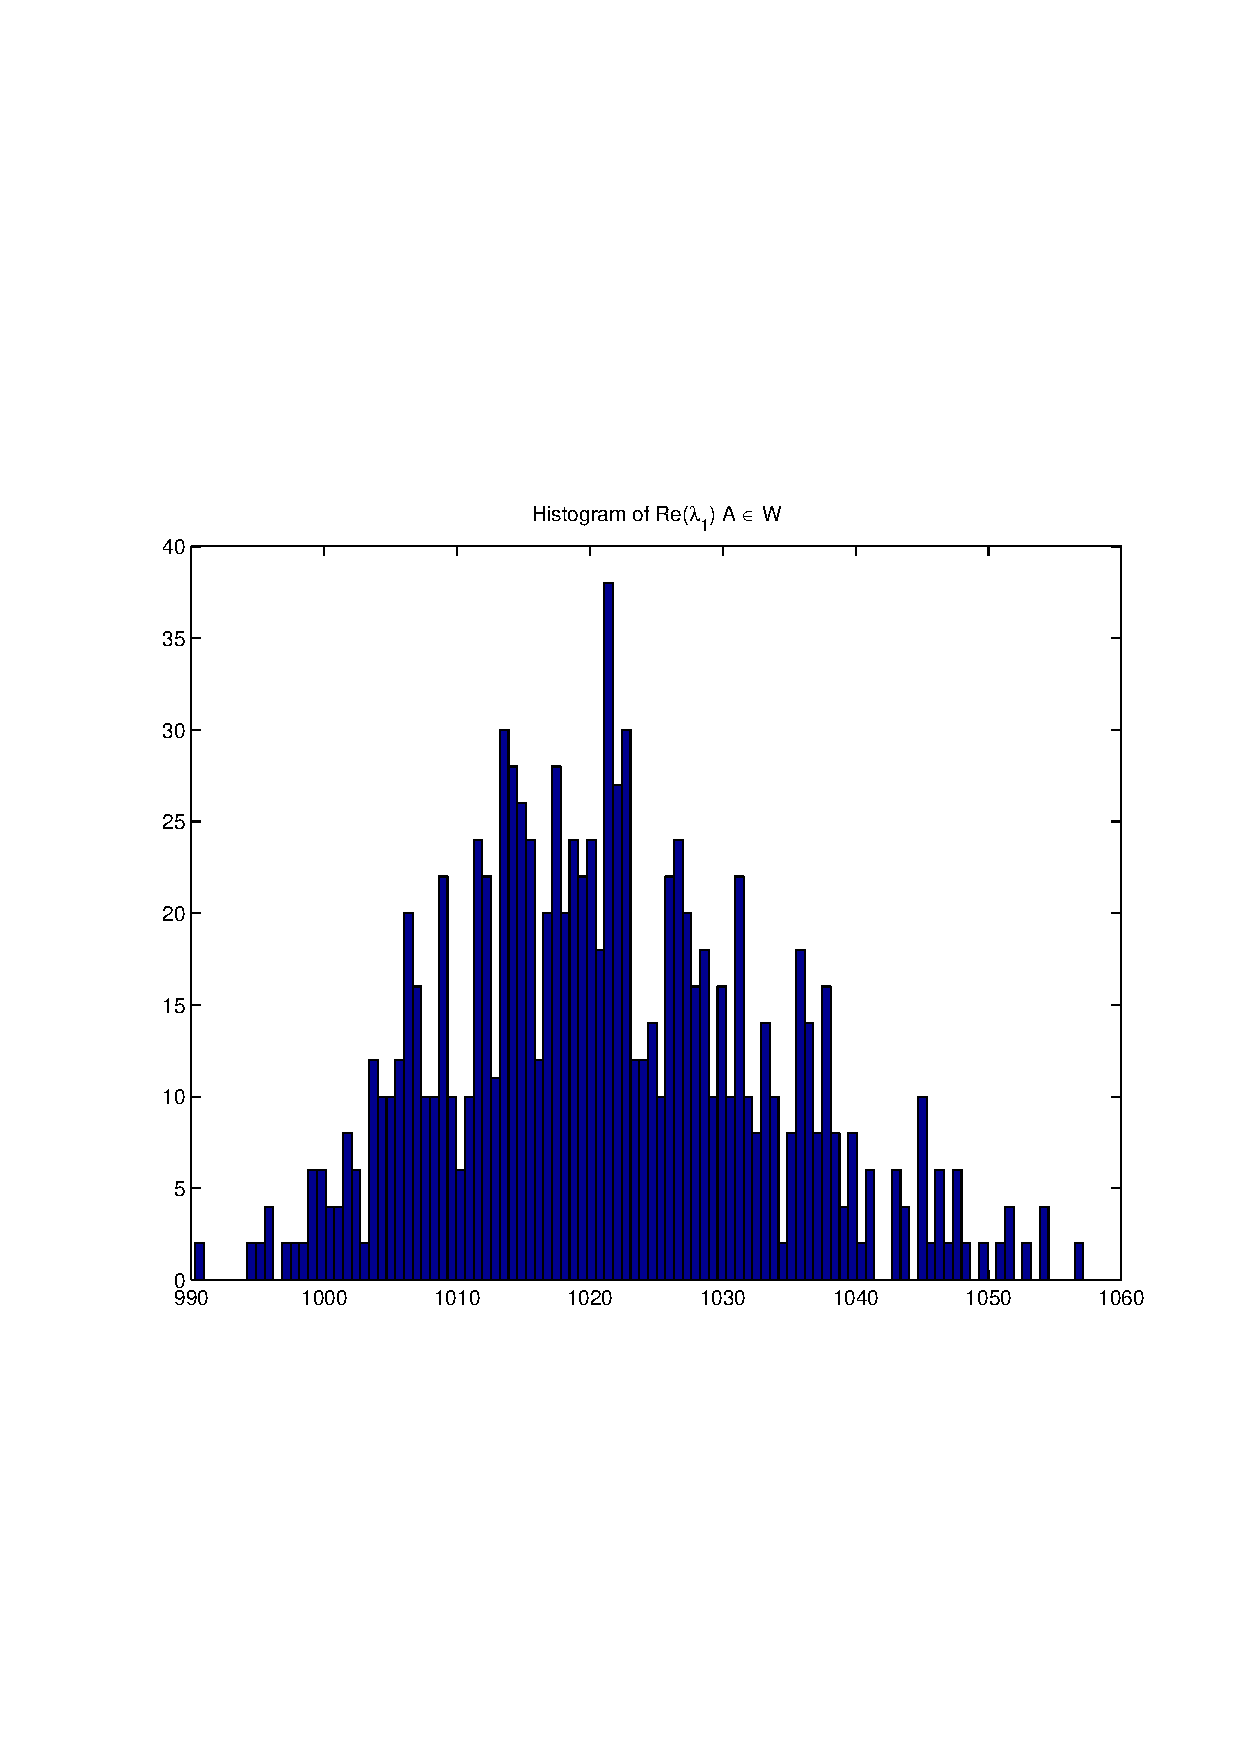
\includegraphics[width=10.0cm,height=10.0cm]{Re_TraceyWidom.pdf}

\includegraphics[width=10.0cm,height=10.0cm]{Im_TraceyWidom.pdf}

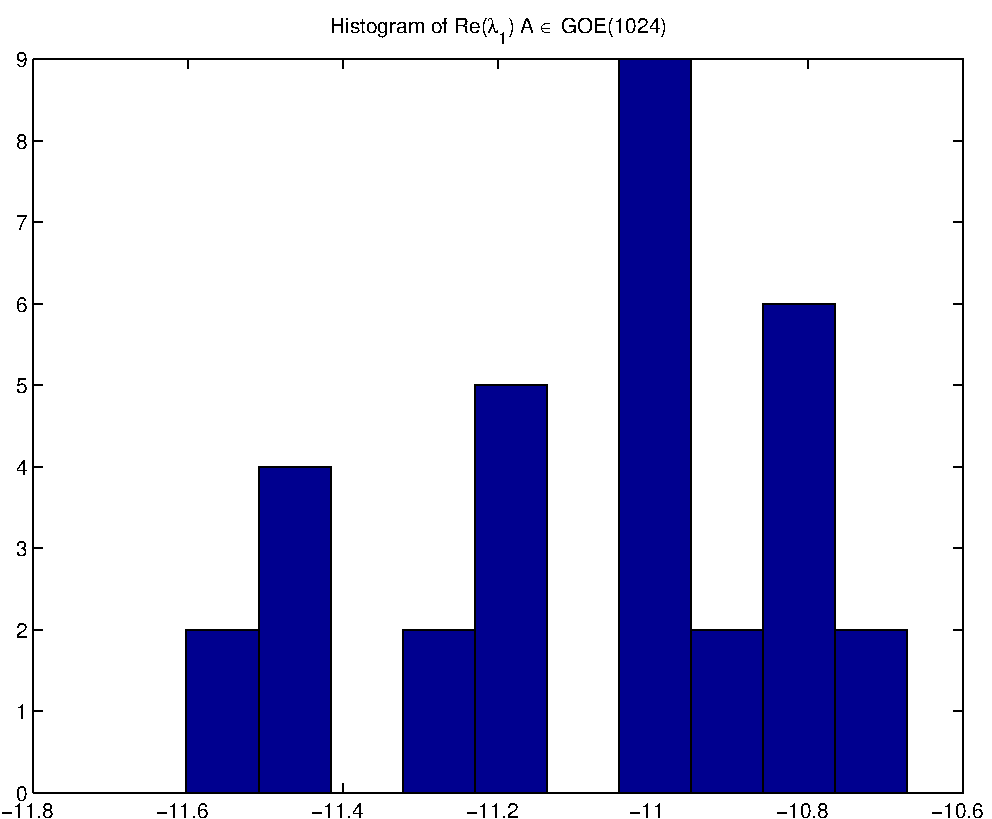
\includegraphics[width=10.0cm,height=10.0cm]{Re_Winger.pdf}

\includegraphics[width=10.0cm,height=10.0cm]{Im_Winger.pdf}

QueryPerformanceCounter  =  +5.477
\subsubsection{Approximate Winger Distribution}
\subsubsection{Verfy Winger Law.}
Let $M_n = [X_{ij} ]$ a symmetric n x n matrix with Random entries such that $X_{i,j} = X_{j,i}$, 		  and $X_{i,j}$ are iid $orall i < j,$ and $Xjj$ are iid $orall j  :  ; E[X^2_{ij} ] = 1, & E[X_{ij}] = 0$ 		  and that all moments exists for each of the entries.  		  The eigenvector of this random matrix; $ lambda_1 leq ... leq lambda_n$ depends continuously on $Mn$.
Dimension $n = +512$

\includegraphics[width=10.0cm,height=10.0cm]{Re_lambda_n.pdf}

\includegraphics[width=10.0cm,height=10.0cm]{Im_lambda_n.pdf}

QueryPerformanceCounter  =  +2.662
\subsubsection{Matrix Exponential }
$SPD Matrix = \left(
\begin{array}{
cccccccc}
+10.539 & -0.499 & -0.010 & +0.368 & +0.465 & -0.492 & -0.126 & +0.437 \\
-0.499 & +7.286 & +0.365 & -0.481 & -0.337 & -0.466 & +0.279 & +0.056 \\
-0.010 & +0.365 & +6.705 & -0.205 & +0.467 & +0.131 & +0.077 & -0.089 \\
+0.368 & -0.481 & -0.205 & +6.496 & -0.402 & -0.209 & +0.043 & -0.041 \\
+0.465 & -0.337 & +0.467 & -0.402 & +4.578 & +0.272 & +0.289 & -0.285 \\
-0.492 & -0.466 & +0.131 & -0.209 & +0.272 & +8.181 & +0.343 & -0.244 \\
-0.126 & +0.279 & +0.077 & +0.043 & +0.289 & +0.343 & +5.938 & -0.212 \\
+0.437 & +0.056 & -0.089 & -0.041 & -0.285 & -0.244 & -0.212 & +9.691 \\
\end{array}
\right)$ \newline 

$SPD Eigs = \left(
\begin{array}{
cccccccc}
(+10.93611,+0.00000) & (+9.60778,+0.00000) & (+4.23666,+0.00000) & (+8.36911,+0.00000) & (+7.56229,+0.00000) & (+5.82791,+0.00000) & (+6.54198,+0.00000) & (+6.33139,+0.00000) \\
\end{array}
\right)$ \newline 

$exp(SPD) = \left(
\begin{array}{
cccccccc}
+47863.969 & -6460.093 & -1078.770 & +4706.958 & +2535.224 & -8475.398 & -2406.368 & +12977.552 \\
-6460.093 & +2780.574 & +516.920 & -1069.918 & -548.083 & -109.707 & +386.466 & -807.216 \\
-1078.770 & +516.920 & +1015.281 & -385.755 & +176.069 & +458.541 & +212.284 & -859.022 \\
+4706.958 & -1069.918 & -385.755 & +1267.210 & +111.181 & -1018.272 & -287.809 & +1036.628 \\
+2535.224 & -548.083 & +176.069 & +111.181 & +413.265 & +135.193 & +45.490 & -502.411 \\
-8475.398 & -109.707 & +458.541 & -1018.272 & +135.193 & +5613.026 & +968.003 & -4270.737 \\
-2406.368 & +386.466 & +212.284 & -287.809 & +45.490 & +968.003 & +632.432 & -1645.725 \\
+12977.552 & -807.216 & -859.022 & +1036.628 & -502.411 & -4270.737 & -1645.725 & +19362.944 \\
\end{array}
\right)$ \newline 

$exp(SPD) eigs = \left(
\begin{array}{
cccccccc}
(+56168.17045,+0.00000) & (+14880.07985,+0.00000) & (+4311.77579,+0.00000) & (+1924.25027,+0.00000) & (+69.17669,+0.00000) & (+339.64809,+0.00000) & (+693.66208,+0.00000) & (+561.93669,+0.00000) \\
\end{array}
\right)$ \newline 

$log(exp(SPD) eigs)  = \left(
\begin{array}{
cccccccc}
(+10.93611,+0.00000) & (+9.60778,+0.00000) & (+8.36911,+0.00000) & (+7.56229,+0.00000) & (+4.23666,+0.00000) & (+5.82791,+0.00000) & (+6.54198,+0.00000) & (+6.33139,+0.00000) \\
\end{array}
\right)$ \newline 

$exp(Id) = \left(
\begin{array}{
cccccccc}
+2.718 & +0.000 & +0.000 & +0.000 & +0.000 & +0.000 & +0.000 & +0.000 \\
+0.000 & +2.718 & +0.000 & +0.000 & +0.000 & +0.000 & +0.000 & +0.000 \\
+0.000 & +0.000 & +2.718 & +0.000 & +0.000 & +0.000 & +0.000 & +0.000 \\
+0.000 & +0.000 & +0.000 & +2.718 & +0.000 & +0.000 & +0.000 & +0.000 \\
+0.000 & +0.000 & +0.000 & +0.000 & +2.718 & +0.000 & +0.000 & +0.000 \\
+0.000 & +0.000 & +0.000 & +0.000 & +0.000 & +2.718 & +0.000 & +0.000 \\
+0.000 & +0.000 & +0.000 & +0.000 & +0.000 & +0.000 & +2.718 & +0.000 \\
+0.000 & +0.000 & +0.000 & +0.000 & +0.000 & +0.000 & +0.000 & +2.718 \\
\end{array}
\right)$ \newline 

$exp(Id) eigs = \left(
\begin{array}{
cccccccc}
(+2.71828,+0.00000) & (+2.71828,+0.00000) & (+2.71828,+0.00000) & (+2.71828,+0.00000) & (+2.71828,+0.00000) & (+2.71828,+0.00000) & (+2.71828,+0.00000) & (+2.71828,+0.00000) \\
\end{array}
\right)$ \newline 

$log(exp(Id) eigs)  = \left(
\begin{array}{
cccccccc}
(+1.00000,+0.00000) & (+1.00000,+0.00000) & (+1.00000,+0.00000) & (+1.00000,+0.00000) & (+1.00000,+0.00000) & (+1.00000,+0.00000) & (+1.00000,+0.00000) & (+1.00000,+0.00000) \\
\end{array}
\right)$ \newline 

For $n  \in  \dblz [16,128)$ we calculate  $|( SPD(n) Eigs - log(exp(SPD(n)) eigs)|_{l^2}$

$|( SPD(n) Eigs - log(exp(SPD(n)) eigs)|_{l^2} = \left(
\begin{array}{
cccccccccccccccccccccccccccccccccccccccccccccccccccccccccccccccccccccccccccccccccccccccccccccccccccccccccccccccc}
(+5.36543,+0.00000) & (+5.36543,+0.00000) & (+5.36543,+0.00000) & (+5.36543,+0.00000) & (+5.36543,+0.00000) & (+5.36543,+0.00000) & (+5.36543,+0.00000) & (+5.36543,+0.00000) & (+5.36543,+0.00000) & (+5.36543,+0.00000) & (+5.36543,+0.00000) & (+5.36543,+0.00000) & (+5.36543,+0.00000) & (+5.36543,+0.00000) & (+5.36543,+0.00000) & (+5.36543,+0.00000) & (+5.36543,+0.00000) & (+5.36543,+0.00000) & (+5.36543,+0.00000) & (+5.36543,+0.00000) & (+5.36543,+0.00000) & (+5.36543,+0.00000) & (+5.36543,+0.00000) & (+5.36543,+0.00000) & (+5.36543,+0.00000) & (+5.36543,+0.00000) & (+5.36543,+0.00000) & (+5.36543,+0.00000) & (+5.36543,+0.00000) & (+5.36543,+0.00000) & (+5.36543,+0.00000) & (+5.36543,+0.00000) & (+5.36543,+0.00000) & (+5.36543,+0.00000) & (+5.36543,+0.00000) & (+5.36543,+0.00000) & (+5.36543,+0.00000) & (+5.36543,+0.00000) & (+5.36543,+0.00000) & (+5.36543,+0.00000) & (+5.36543,+0.00000) & (+5.36543,+0.00000) & (+5.36543,+0.00000) & (+5.36543,+0.00000) & (+5.36543,+0.00000) & (+5.36543,+0.00000) & (+5.36543,+0.00000) & (+5.36543,+0.00000) & (+0.00000,+0.00000) & (+0.00000,+0.00000) & (+0.00000,+0.00000) & (+0.00000,+0.00000) & (+0.00000,+0.00000) & (+0.00000,+0.00000) & (+0.00000,+0.00000) & (+0.00000,+0.00000) & (+0.00000,+0.00000) & (+0.00000,+0.00000) & (+0.00000,+0.00000) & (+0.00000,+0.00000) & (+0.00000,+0.00000) & (+0.00000,+0.00000) & (+0.00000,+0.00000) & (+0.00000,+0.00000) & (+0.00000,+0.00000) & (+0.00000,+0.00000) & (+0.00000,+0.00000) & (+0.00000,+0.00000) & (+0.00000,+0.00000) & (+0.00000,+0.00000) & (+0.00000,+0.00000) & (+0.00000,+0.00000) & (+0.00000,+0.00000) & (+0.00000,+0.00000) & (+0.00000,+0.00000) & (+0.00000,+0.00000) & (+0.00000,+0.00000) & (+0.00000,+0.00000) & (+0.00000,+0.00000) & (+0.00000,+0.00000) & (+0.00000,+0.00000) & (+0.00000,+0.00000) & (+0.00000,+0.00000) & (+0.00000,+0.00000) & (+0.00000,+0.00000) & (+0.00000,+0.00000) & (+0.00000,+0.00000) & (+0.00000,+0.00000) & (+0.00000,+0.00000) & (+0.00000,+0.00000) & (+0.00000,+0.00000) & (+0.00000,+0.00000) & (+0.00000,+0.00000) & (+0.00000,+0.00000) & (+0.00000,+0.00000) & (+0.00000,+0.00000) & (+0.00000,+0.00000) & (+0.00000,+0.00000) & (+0.00000,+0.00000) & (+0.00000,+0.00000) & (+0.00000,+0.00000) & (+0.00000,+0.00000) & (+0.00000,+0.00000) & (+0.00000,+0.00000) & (+0.00000,+0.00000) & (+0.00000,+0.00000) & (+0.00000,+0.00000) & (+0.00000,+0.00000) & (+0.00000,+0.00000) & (+0.00000,+0.00000) & (+0.00000,+0.00000) & (+0.00000,+0.00000) \\
\end{array}
\right)$ \newline 

QueryPerformanceCounter  =  +0.00949
The sample size generated for this run is 100000.

\newpage
uniform \begin{tabular}{|c|c|c|c|}  mean & variance & skewness & kurtosis \\  \hline
$\mu_1 = +0.50030$ & $\mu_2 = +0.08353$ & $\mu_3 = +0.00339$ & $\mu_4 =+1.80113$ \\
\end{tabular}

\includegraphics[width=5cm,height=5cm]{uniform.pdf}

cauchy \begin{tabular}{|c|c|c|c|}  mean & variance & skewness & kurtosis \\  \hline
$\mu_1 = +0.44288$ & $\mu_2 = +0.05341$ & $\mu_3 = +0.63935$ & $\mu_4 =+3.28094$ \\
\end{tabular}

\includegraphics[width=5cm,height=5cm]{cauchy.pdf}

exponential \begin{tabular}{|c|c|c|c|}  mean & variance & skewness & kurtosis \\  \hline
$\mu_1 = +1.99647$ & $\mu_2 = +3.99339$ & $\mu_3 = +2.03097$ & $\mu_4 =+9.30842$ \\
\end{tabular}

\includegraphics[width=5cm,height=5cm]{exponential.pdf}

\newpage
gamma \begin{tabular}{|c|c|c|c|}  mean & variance & skewness & kurtosis \\  \hline
$\mu_1 = +1.89088$ & $\mu_2 = +1.89784$ & $\mu_3 = +1.49318$ & $\mu_4 =+6.39583$ \\
\end{tabular}

\includegraphics[width=5cm,height=5cm]{gamma.pdf}

GIG \begin{tabular}{|c|c|c|c|}  mean & variance & skewness & kurtosis \\  \hline
$\mu_1 = +0.81394$ & $\mu_2 = +11.71052$ & $\mu_3 = +15.06978$ & $\mu_4 =+303.44946$ \\
\end{tabular}

\includegraphics[width=5cm,height=5cm]{GIG.pdf}

normal-box-muller \begin{tabular}{|c|c|c|c|}  mean & variance & skewness & kurtosis \\  \hline
$\mu_1 = +0.00043$ & $\mu_2 = +1.00470$ & $\mu_3 = -0.00561$ & $\mu_4 =+2.99650$ \\
\end{tabular}

\includegraphics[width=5cm,height=5cm]{normal-box-muller.pdf}

\newpage
normal-inverse-approximation \begin{tabular}{|c|c|c|c|}  mean & variance & skewness & kurtosis \\  \hline
$\mu_1 = +0.00230$ & $\mu_2 = +1.00486$ & $\mu_3 = +0.01163$ & $\mu_4 =+2.99254$ \\
\end{tabular}

\includegraphics[width=5cm,height=5cm]{normal-inverse-approximation.pdf}

pareto \begin{tabular}{|c|c|c|c|}  mean & variance & skewness & kurtosis \\  \hline
$\mu_1 = +3184578.26493$ & $\mu_2 = +888468246174112900.00000$ & $\mu_3 = +315.36997$ & $\mu_4 =+99629.09819$ \\
\end{tabular}

\includegraphics[width=5cm,height=5cm]{pareto.pdf}

poisson \begin{tabular}{|c|c|c|c|}  mean & variance & skewness & kurtosis \\  \hline
$\mu_1 = +1.10585$ & $\mu_2 = +0.13283$ & $\mu_3 = +3.97542$ & $\mu_4 =+21.69590$ \\
\end{tabular}

\includegraphics[width=5cm,height=5cm]{poisson.pdf}

\newpage
beta \begin{tabular}{|c|c|c|c|}  mean & variance & skewness & kurtosis \\  \hline
$\mu_1 = +0.33319$ & $\mu_2 = +0.12696$ & $\mu_3 = +0.67978$ & $\mu_4 =+1.90795$ \\
\end{tabular}

\includegraphics[width=5cm,height=5cm]{beta.pdf}

QueryPerformanceCounter  =  +11.06168
\subsubsection{Multiclass Support Vector Machine }
\begin{itemize}
\item Number or training points = 1024
\item Feature dimension = 3
\item Number or classes = 3
\end{itemize}
{The mean vectors of the 3 classes}

$\mu_1 = \left(
\begin{array}{
ccc}
+1.90000 & +0.10000 & +0.10000 \\
\end{array}
\right)$ \newline 

$\mu_2 = \left(
\begin{array}{
ccc}
+0.10000 & +1.90000 & +0.10000 \\
\end{array}
\right)$ \newline 

$\mu_3 = \left(
\begin{array}{
ccc}
+0.00000 & +0.00000 & +1.90000 \\
\end{array}
\right)$ \newline 

A random SPD covairance matrix is generated for each of the classes.\newline

$\rho_1 = \left(
\begin{array}{
ccc}
+2.020 & +0.069 & -0.032 \\
+0.069 & +1.629 & +0.499 \\
-0.032 & +0.499 & +1.561 \\
\end{array}
\right)$ \newline 

$\rho_2 = \left(
\begin{array}{
ccc}
+2.386 & +0.057 & -0.324 \\
+0.057 & +3.953 & -0.019 \\
-0.324 & -0.019 & +2.771 \\
\end{array}
\right)$ \newline 

$\rho_3 = \left(
\begin{array}{
ccc}
+2.042 & +0.333 & -0.189 \\
+0.333 & +2.697 & -0.199 \\
-0.189 & -0.199 & +2.592 \\
\end{array}
\right)$ \newline 

Verify $L_1$ condition number of covariance. The diagonal entries of the matrix have the form $(0.5 + U(0,1) )*dim(Dom(Cov))$
The lower-diagonal entries take the form $U(0,1) - 0.5$. 
The $L_1$ condition numbers are :
\begin{itemize}
\item +2.083
\item +1.941
\item +1.918
\end{itemize}
\includegraphics[width=10.0cm,height=10.0cm]{rv1_corr.pdf}

\includegraphics[width=10.0cm,height=10.0cm]{rv2_corr.pdf}

\includegraphics[width=10.0cm,height=10.0cm]{rv3_corr.pdf}

\includegraphics[width=10.0cm,height=10.0cm]{trainingPoints.pdf}

These are the SVM parameters - the RBF kernel is used\begin{itemize}
\item allOutlierFraction=0.05
\item mixingCoeff=0.3
\item smoThresh=1.0/10000.0
\item sigma=1
\end{itemize}
\includegraphics[width=10.0cm,height=10.0cm]{testPoints.pdf}

The marginal sample moments (mean var skew kurtosis) for training points.\newline
\begin{tabular}{ c |  c  c  c  c}
Feature & $\mu_1$ & $\mu_2$ & $\mu_3$ & $\mu_4$ \\
0 & +0.669 & +1.196 & +0.270& +2.196 \\
\hline
1 & +0.703 & +1.257 & +0.597& +2.696 \\
\hline
2 & +0.704 & +1.180 & +0.445& +2.432 \\
\hline
\end{tabular}
\newline
The marginal sample moments (mean var skew kurtosis) for test points.\newline
\begin{tabular}{ c | c  c  c  c}
Feature & $\mu_1$ & $\mu_2$ & $\mu_3$ & $\mu_4$ \\
0 & +0.676 & +1.121 & +0.402& +2.257\\
\hline
1 & +0.673 & +1.243 & +0.634& +2.677\\
\hline
2 & +0.715 & +1.136 & +0.414& +2.387\\
\hline
\end{tabular}\newline
\includegraphics[width=10.0cm,height=10.0cm]{classDiffs.pdf}

The error rate for this run is +0.083\newline
QueryPerformanceCounter  =  +6.318
\subsubsection{Semidefinite Programming SDPA}
QueryPerformanceCounter  =  +0.006
\end{document}
